\documentclass[11pt]{article} 
% These materials are licensed under the Creative Commons CC: BY NC SA license. Please see: https://creativecommons.org/licenses/by-nc-sa/2.0/
% The IODE team:
% Chris Rasmussen
% Karen Allen Keene
% Justin Dunmyre
% Nicholas Fortune

% Special thanks to Mariah Birgen for her efforts in making a huge first effort in TeXing the previous version of the IODE materials.

%This version of the materials was last updated on July 21, 2020.

%%%%%%%%%%%%%%%%%%%%%%%%%%%%%%%%%%%%%%%%%%%%%%%%%%%
%					CUSTOMIZING YOUR PDF									%
%																			%
%	All of the easy customizations are in this box										%
%																			%
%	IMPORTANT: If you make any changes to the materials you should compile IODE.tex twice	%
%																			%
%																			%
%																			%
%					CUSTOMIZING YOUR PAGE NUMBERING						%
%																			%
%  	*Exactly* one of the following \newcommand lines									%
%	should NOT have a % sign in front of it 											%
%																			%
%      Our predefined page numbering styles are explained here,							%
%	you may change them to fit your needs											% 
%																			%
%																			%
%     Book page numbering:														%
%     Unit 1 starts on page 1, Unit 2 starts on the page n+1, where n is the last page of Unit 1.		%
     
%\newcommand{\BookPageNumbers}{Page \thepage}     
     
%	Unit page numbering:														%
%	Unit 1's pages are 1.1, 1.2, etc, and Unit 2's pages are 2.1, 2.2, etc.						%
     
\newcommand{\UnitPageNumbers}{Page \theUnit.\thepage}      

%	No page numbering:															%
%	Pages are not numbered.														%

%\newcommand{\NoPageNumbers}{}

%																			%
%					PRINTING ONE SECTION AT A TIME							%
%	First, compile the document with the following line with the % in front of it.	Then				%
%	remove the % in front of the following line and change it to the section that you want to show.	%
%	For example, if you wanted to only show unit 9, you'd change the 01/01 to 09/09			%
%	Chapter files need to be in subfolders labeled 01-14									%
%																			%
%	If you wish to use the includeonly function but have made significant changes to the materials,	%
%	you first need to comment out the includeonly function and compile IODE.tex to ensure all 	%
%	page numbering and problem references are accurate.								%

\includeonly{01/01}

%																			%
%%%%%%%%%%%%%%%%%%%%%%%%%%%%%%%%%%%%%%%%%%%%%%%%%%%

\usepackage[margin=.75in,top=.75in,bottom=1.25in,headsep=5pt,headheight=5pt]{geometry}
\usepackage{fancyhdr}
\usepackage{amsmath}
\usepackage{amsthm}
\usepackage{amsfonts}
\usepackage{graphicx}
\usepackage{tabularx}
\usepackage{mathrsfs}
\usepackage{framed}
\usepackage{tikz}
\usepackage{hyperref} % to get hyper links in materials
\usepackage[inline]{enumitem} % gives ability to continue with numbering (add [resume] after \begin{enumerate}) AND to make horizontal lists by adding * to enumerate (\begin{enumerate*})
\usepackage{verbatim}  % for the comment environment
\usepackage{xcolor} %for color on cover page
\usepackage{ifthen}
\newcommand{\degree}{$^{\circ}$}

\newcommand{\theUnit}{0}


\newcommand{\mypage}{
\ifthenelse{\isundefined{\BookPageNumbers}}{}{\BookPageNumbers}
\ifthenelse{\isundefined{\UnitPageNumbers}}{}{\UnitPageNumbers}
\ifthenelse{\isundefined{\NoPageNumbers}}{}{\NoPageNumbers}
}

%%%%%%%%%%%%%%%%%%%%%%%%%%%%%%%%%%%%%%%%
%This function was previously used when the teacher materials were part of the materials but they are now separate so this function is no longer used*
\newenvironment{TM}[1]%
        {%
            \ifthenelse{\isundefined{\showTM}}%
                    {\expandafter\comment}%
                    {\begin{framed}\begin{center}\textbf{#1}\end{center}}%
                    }
         {%
            \ifthenelse{\isundefined{\showTM}}%
                    {\expandafter\endcomment}%
                    {\end{framed}}%
          }
%%%%%%%%%%%%%%%%%%%%%%%%%%%%%%%%%%%%%%%%

\newcommand{\pagebegin}[1]{\section{#1}}
\setcounter{secnumdepth}{0}

\newcounter{probno}[enumi]
\newcommand{\hitem}{\hfill \stepcounter{probno} (\roman{probno})\hspace{1em}}
\newenvironment{hnumerate}{\begin{center}}{\hfill\setcounter{probno}{0}\end{center}}

\newcounter{eqnno}[enumi]
\newcommand{\eqn}{\stepcounter{eqnno} (\theeqnno) \label{05table\theeqnno}}
\newcommand{\vs}{\vskip.2cm} %customizable command for inserting small vertical space.  Usually appears between paragraphs.



\begin{document}
\setlength\parindent{0pt}
\title{Inquiry Oriented Differential Equations}
\setcounter{page}{1}
%\tableofcontents
\clearpage
%IODE COVER PAGE
%%%%%%%%%%%%%%%%%%%%%%%%%%%
%%%% Put the following at the top of each .tex file  %
\pagestyle{fancy}
\renewcommand{\theUnit}{1}
\ifthenelse{\isundefined{\UnitPageNumbers}}{}{\setcounter{page}{0}}
\rhead{}
\lhead{}
\rfoot{\raisebox{.3em}{\href{https://iode.wordpress.ncsu.edu}{\underline{https://iode.sdsu.edu}}}}
\lfoot{
\includegraphics[width=1.5cm]{CopyrightCCBYNCSA.pdf} \raisebox{.3em}{The IODE Team}}
\cfoot{\raisebox{.3em}{Last Update: December 22, 2022}}
\fancypagestyle{firstfooter}{\footskip = 50pt}
\renewcommand{\footrulewidth}{.4pt}
%%%%%%%%%%%%%%%%%%%%%%%%%%%
\vspace*{-20pt} \thispagestyle{firstfooter}
\pagebegin{}
\begin{center}\Huge{INQUIRY ORIENTED \\ DIFFERENTIAL EQUATIONS}\end{center}
\vspace{.5in}
\begin{center}

\includegraphics[width=6in]{IODE-logo-coverpage.png}
\end{center}
\vspace{.75in}
\begin{center}
\begin{tabular}{c|ll}
 & \LARGE{Chris Rasmussen} & \color{black!60}{\textit{San Diego State University}} \\
&& \\
 & \LARGE{Karen Allen Keene} & \color{black!60}{\textit{Embry-Riddle Aeronautical University}} \\
&& \\
 & \LARGE{Justin Dunmyre} & \color{black!60}{\textit{Frostburg State University}} \\
&& \\
 & \LARGE{Nicholas Fortune} & \color{black!60}{\textit{Western Kentucky University}} \\
\end{tabular}
\end{center}
\vspace{-1.6in}\hspace{1in}\rotatebox{90}{\large{\textbf{\color{red}{The IODE Team}}}}


%UNIT 1: QUALITATIVE AND GRAPHICAL APPROACHES
%%%%%%%%%%%%%%%%%%%%%%%%%%%
%%%% Put the following at the top of each .tex file  %
\pagestyle{fancy}
\renewcommand{\theUnit}{1}
\ifthenelse{\isundefined{\UnitPageNumbers}}{}{\setcounter{page}{1}}
\rhead{Unit \theUnit: Qualitative and Graphical Approaches}
\lhead{
\includegraphics[width=1.25cm]{IODE-logo.png}}
\rfoot{\mypage}
\lfoot{}
\cfoot{}
\fancypagestyle{firstfooter}{\footskip = 50pt}
\renewcommand{\footrulewidth}{.4pt}
%%%%%%%%%%%%%%%%%%%%%%%%%%%
\vspace*{-20pt} \thispagestyle{firstfooter}
\pagebegin{Bees and Flowers}

Often scientists use rate of change equations in their study of population growth for one or more species. In this problem we study systems of rate of change equations designed to inform us about the future populations for two species that are either competitive (that is, both species are \textsl{harmed by} interaction) or cooperative (that is, both species \textsl{benefit from} interaction).
\vs
\begin{enumerate}
\item Which system of rate of change equations below describes a situation where the two species compete and which system describes cooperative species? Explain your reasoning. \label{01problem1}

	\begin{center}
(i)	$  \displaystyle \begin{aligned}[t]
        \frac{dx}{dt} &= -5x +2xy\\
        \frac{dy}{dt} &= -4y +3xy
        \end{aligned}$	\hspace{1.5in}
    (ii) $  \displaystyle \begin{aligned}[t]
        \frac{dx}{dt} &= 4x -2xy\\
        \frac{dy}{dt} &= 2y - xy
        \end{aligned}$
\end{center}
\end{enumerate}

\clearpage
%%%%%%%%%%%%%%%%%
\pagebegin{A Simplified Situation}

The previous problem dealt with a complex situation with two interacting species. To develop the ideas and tools that we will need to further analyze complex situations like these, we will simplify the situation by making the following assumptions:

\begin{itemize}
\item	There is only one species ({\em e.g.}, fish)
\item	The species has been in its habitat ({\em e.g.}, a lake) for some time prior to what we call $t = 0$
\item	The species has access to unlimited resources ({\em e.g.}, food, space, water) 
\item	The species reproduces continuously

\end{itemize}
\begin{enumerate}[resume]
\item	Given these assumptions for a certain lake containing fish, sketch three possible population versus time graphs: one starting at $P = 10$, one starting at $P = 20$, and the third starting at $P = 30$. \label{01problem2}

\begin{center}
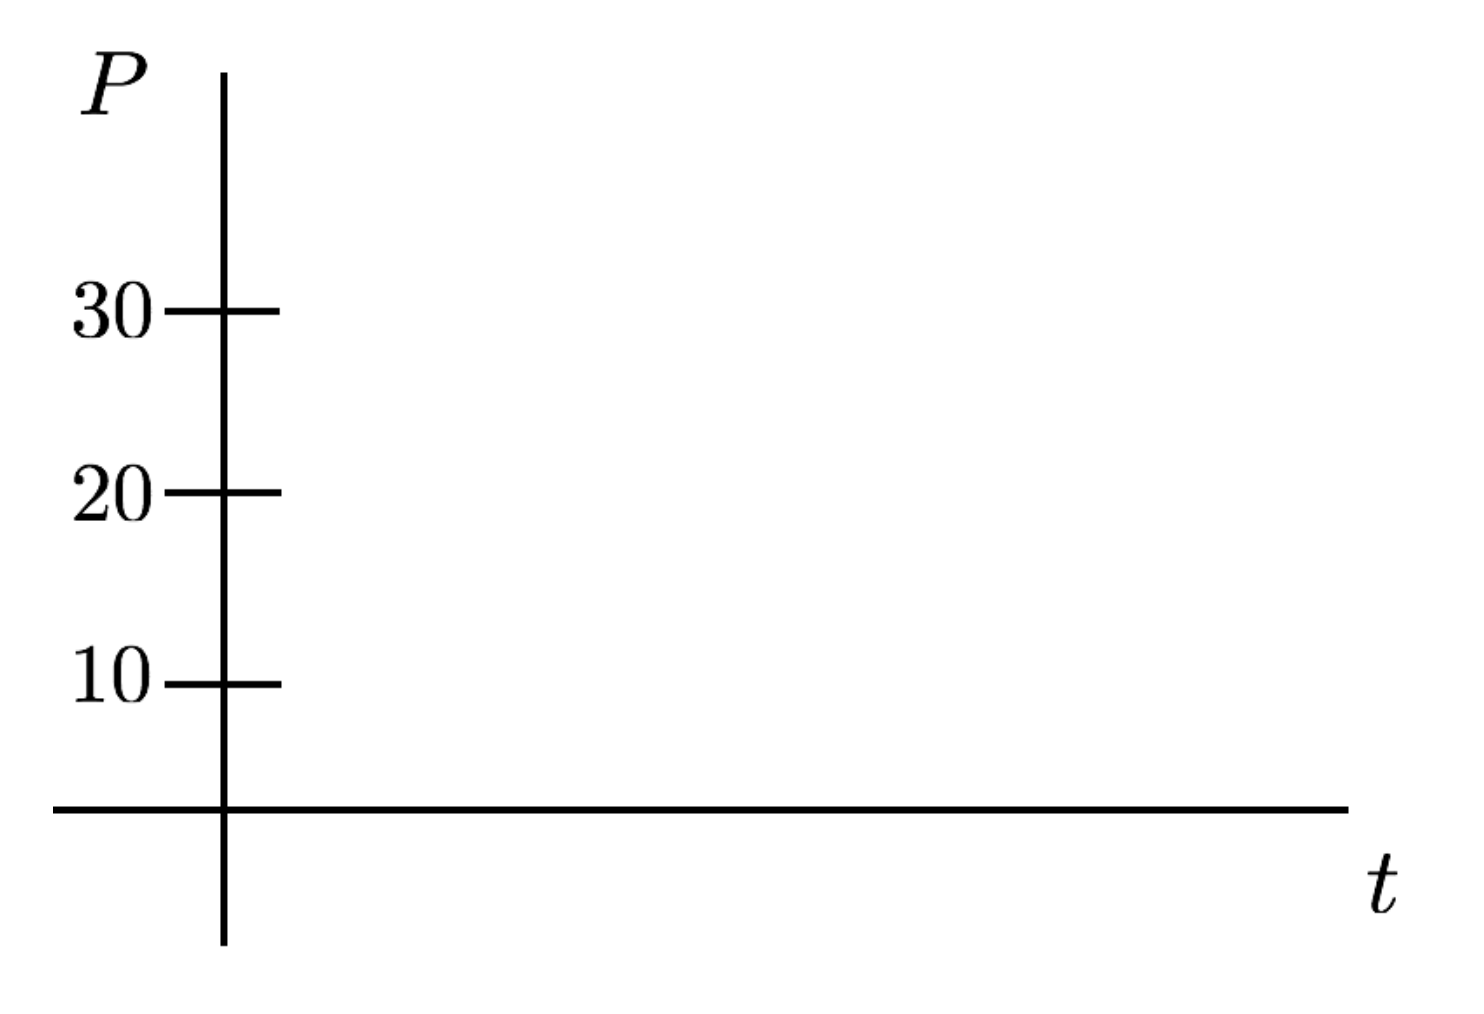
\includegraphics[width=3.5in]{01/01FishGraph.png}
\end{center}
\begin{enumerate}
\item	For your graph starting with $P = 10$, how does the slope vary as time increases? Explain. \label{01problem2parta}
\vfill
\item	For a set $P$ value, say $P = 30$, how do the slopes vary across the three graphs you drew? \label{01problem2partb}
\vfill
\end{enumerate}
\item This situation can also be modeled with a rate of change equation, $\frac{dP}{dt}=something$. What should the ``something'' be? Should the rate of change be stated in terms of just $P$, just $t$, or both $P$ and $t$? Make a conjecture about the right hand side of the rate of change equation and provide reasons for your conjecture. \label{01problem3}
\end{enumerate}
\vfill

\clearpage
 
%%%%%%%%%%%%%%%%%
\pagebegin{What Exactly is a Differential Equation and What are Solutions?}

A {\bf differential equation} is an equation that relates an unknown function to its derivative(s). Suppose $y = y(t)$ is some unknown function, then a differential equation, or rate of change equation, would express the rate of change, $\frac{dy}{dt}$, in terms of $y$ and/or $t$. For example, all of the following are differential equations.  

\[ \frac{dP}{dt}=kP,\qquad \frac{dy}{dt}=y+2t, \qquad \frac{dy}{dt}=t^2+5,\qquad \frac{dy}{dt}=\frac{6y-2}{ty}, \qquad \frac{dy}{dt}=\frac{y^2-1}{t^2+2t}
\]

In particular, these are all examples of \textit{first order} differential equations because only the first derivative appears in the equation. Given a rate of change equation for some unknown function, \textbf{solutions} to this rate of change equation are \textsl{functions} that satisfies the rate change equation. A constant function that satisfies the differential equation is called an \textbf{equilibrium solution}.
\begin{enumerate}[resume]
\item One way to read the differential equation $\frac{dy}{dt} = y+2t$ aloud you would say, ``dee $y$ dee $t$ equals $y$ plus two times $t$.'' However, this does \textbf{not} relate to the \textsl{meaning} of the solution.  How might you read this differential equation \textsl{with meaning}? \vfill

\item \begin{enumerate}
\item Is the function $y=1+t$  a solution to the differential equation $\displaystyle\frac{dy}{dt}=\frac{y^2-1}{t^2+2t}$? How about the function $y=1+2t$?  How about $y = 1$?  Explain your reasoning. \label{01problem4parta} \vfill 

\item	Is the function $y=t^3+2t$    a solution to the differential equation $\displaystyle \frac{dy}{dt}=3y^2+2$?  Why or why not? \label{01problem4partb} \vfill

\end{enumerate}

\item	Figure out all the functions that satisfy the rate of change equation $\displaystyle \frac{dP}{dt}=0.3P$. \\(\textsl{Hint}: read the differential equation with meaning.) \label{01problem5} \vfill

\item	Figure out all of the solutions to the differential equation $\displaystyle\frac{dy}{dt}=t^2+5$. \label{01problem6} \vfill
\end{enumerate}

\clearpage
 %%%%%%%%%%%%%%%%%
\pagebegin{Slope Fields}

A \textbf{slope field} is a graphical representation of a rate of change equation. Given a rate of change equation, if we plug in particular values of $(t,y)$ then $\displaystyle\frac{dy}{dt}$ tells you the slope of the tangent vector to the solution at that point.
\vs
For example, consider the rate of change equation $\displaystyle\frac{dy}{dt}=y+2t$.  At the point (1, 3), the value of $\displaystyle\frac{dy}{dt}$ is 5. Thus, the slope field for this equation would show a vector at the point (1, 3) with slope 5.  A slope field depicts the exact slope of many such vectors, where we take each vector to be uniform length. Slope fields are useful because they provide a graphical approach for obtaining qualitatively correct graphs of the functions that satisfy a differential equation.

\begin{enumerate}[resume]
\item Below is a partially completed slope field for  $\displaystyle \frac{dP}{dt}=0.8P$. \label{01problem7}
\begin{enumerate}
\item	Plot many more tangent vectors to create a slope field. \label{01problem7parta}
\item	Use your slope field to sketch in qualitatively correct graphs of the solution functions that start at $P = 0, 0.5$, and $2$, respectively. Note: the value of $P$ at an initial time (typically $t = 0$) is called an \textbf{initial condition}. \label{01problem7partb}
\item	Recall that a solution to a differential equation is a function that satisfies the differential equation. Explain how the graph with initial condition $P(0) = 1$ can graphically be thought of as a solution to the differential equation when the differential equation is represented by its slope field. \label{01problem7partc}
\end{enumerate}

\begin{center}
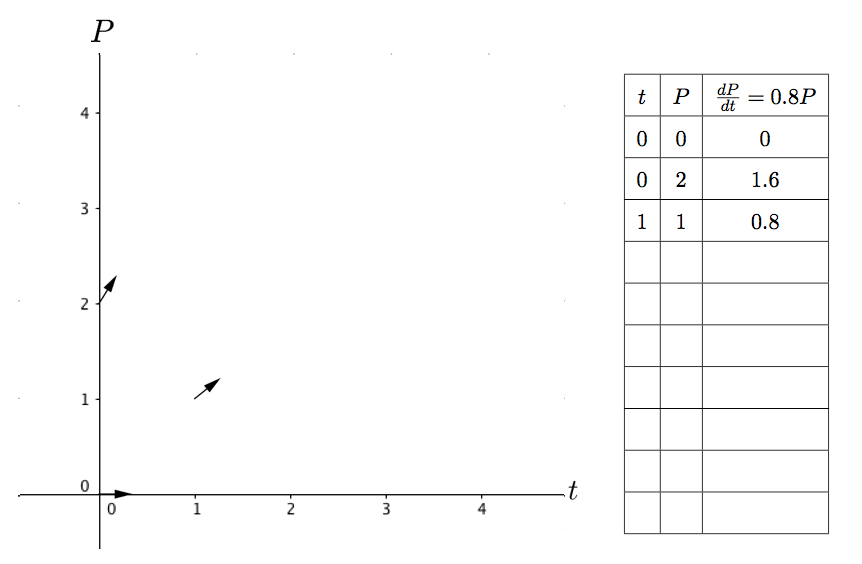
\includegraphics[width=6in]{01/01MyFirstSlopeFieldwithTable.png}
\end{center}

\clearpage

\item Below are seven rate of changes equations and three different slope fields. Without using technology, identify which differential equation is the best match for each slope field (thus you will have four rate of change equations left over). Explain your reasoning. \label{01problem8}
\[
\text{(i) } \frac{dy}{dt}=t-1 \quad \text{(ii) } \frac{dy}{dt}=1-y^2 \quad \text{(iii) } \frac{dy}{dt}=y^2-t^2 \quad \text{(iv) } \frac{dy}{dt}=1-y
\]
\[
\text{(v) } \frac{dy}{dt}=t^2-y^2 \quad \text{(vi) } \frac{dy}{dt}=1-t \quad \text{(vii) } \frac{dy}{dt}=9t^2-y^2
\]
\begin{enumerate*}
\item 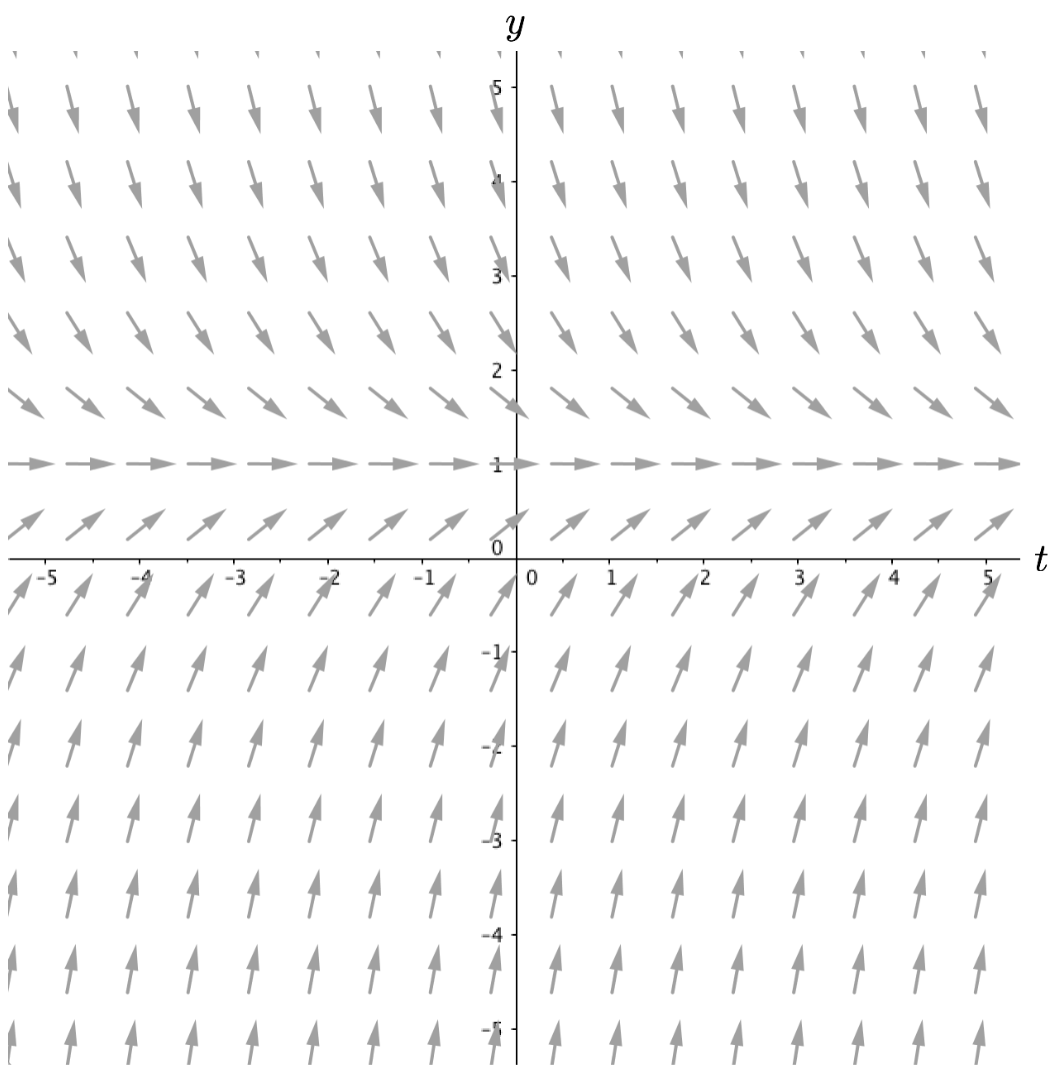
\includegraphics[width=2.75in]{01/01SlopeField1.png} \label{01problem8parta}
\item 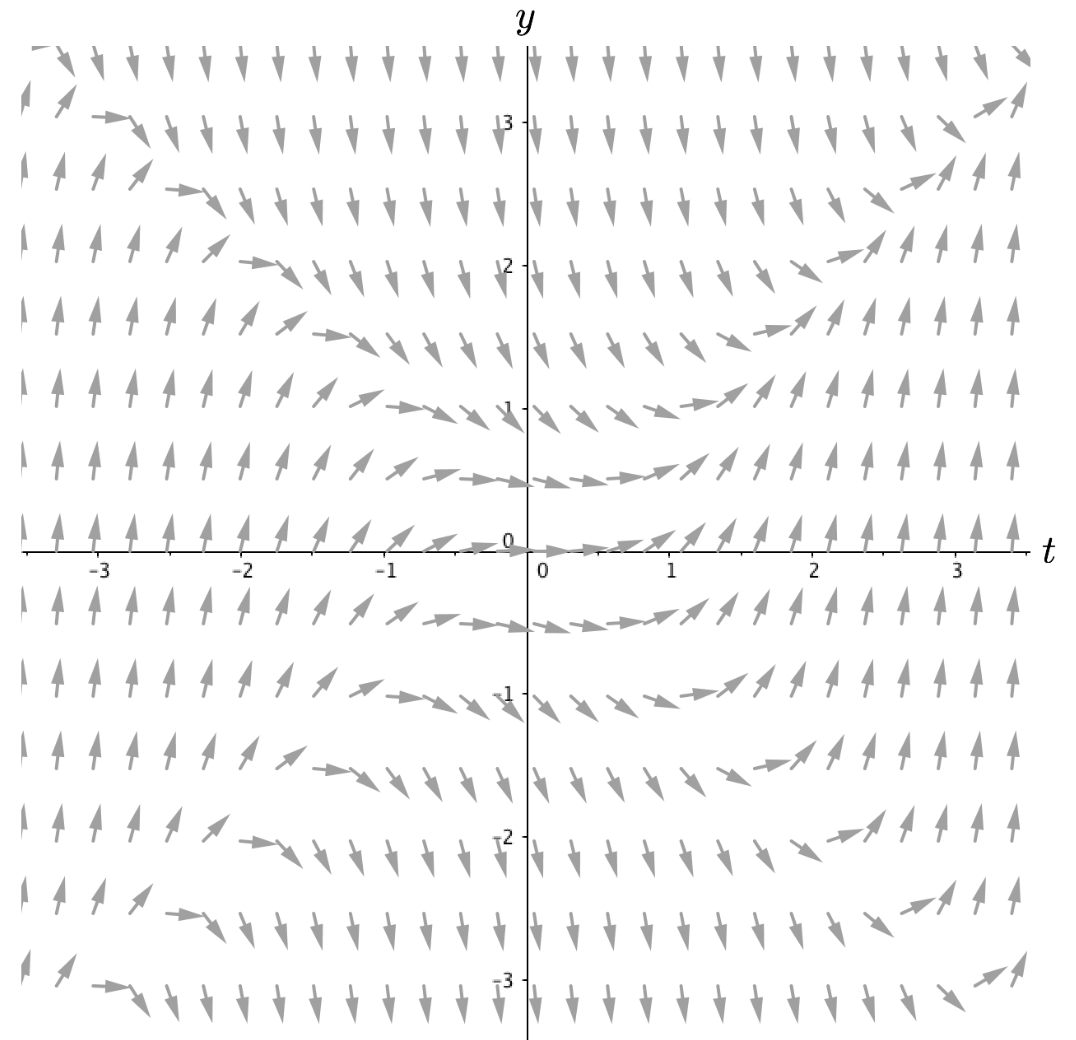
\includegraphics[width=2.75in]{01/01SlopeField2.png} \label{01problem8partb}
\end{enumerate*}

\begin{enumerate*}[resume]
\item 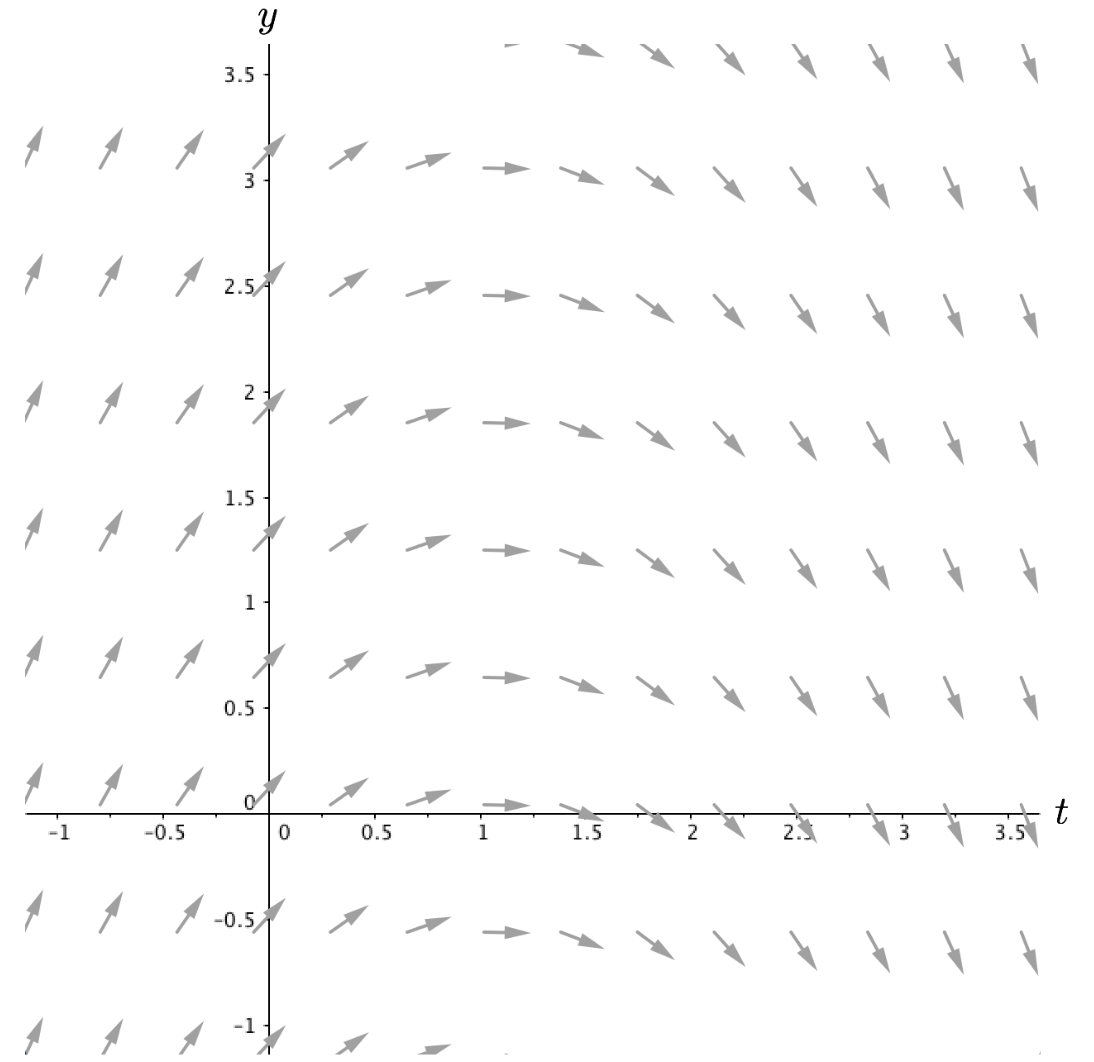
\includegraphics[width=2.75in]{01/01SlopeField3.png} \label{01problem8partc}
\end{enumerate*}
\vspace{0.1in}
\item For each of the slope fields in the previous problem, sketch in graphs of several different qualitatively correct solutions. \label{01problem9}
\vfill

\end{enumerate}
\clearpage

%%%%%%%%%%%%%%%%%
\pagebegin{Homework Set 1}
 
\begin{enumerate}

\item	Consider the following systems of rate of change equations: \label{01HWproblem1}

\begin{center}
\begin{tabular}{cp{1cm}c}
\textbf{System A}	&& \textbf{System B}  \\

$\displaystyle \begin{aligned}[t]
        \frac{dx}{dt} &= 3x\left(1-\frac{x}{10}\right)-20xy\\
        \frac{dy}{dt} &= -5y+\frac{xy}{20}
        \end{aligned}$	&&				
 $  \displaystyle \begin{aligned}[t]
        \frac{dx}{dt} &= 0.3x -\frac{xy}{100}\\
        \frac{dy}{dt} &= 15y\left(1-\frac{y}{17}\right) +25xy
        \end{aligned}$
\end{tabular}	
\end{center}		 

In both of these systems, $x$ and $y$ refer to the number of two different species at time $t$. In particular, in one of these systems the prey are large animals and the predators are small animals, such as piranhas and humans. Thus it takes many predators to eat one prey, but each prey eaten is a tremendous benefit for the predator population. The other system has very large predators and very small prey. \\

Figure out which system is which and explain the reasoning behind your decision. 

\item Consider the rate of change equation  \[ \frac{dy}{dt}=0.5y(2+y)(y-8),\] which has been created to provide predictions about the future population of rabbits over time.  
\begin{enumerate}
\item	For what values of $y$ is $y(t)$ increasing?  Explain your reasoning.
\item	For what values of $y$ is $y(t)$ decreasing?  Explain your reasoning.
\item	For what values of $y$ is $\displaystyle \frac{dy}{dt}$  neither positive nor negative?  What does this imply about the solution function $y(t)$? \label{01HWproblem2}
\end{enumerate}

\item Valeria created the following graph to help her analyze solutions to the differential equation $\displaystyle \frac{dy}{dt} = 2y \left(1-\frac{y}{10} \right)$. What is this a graph of ({\em i.e.}, what are the axes for this graph)? What information about solutions can you glean from this graph? \label{01HWproblem3}
\begin{center}
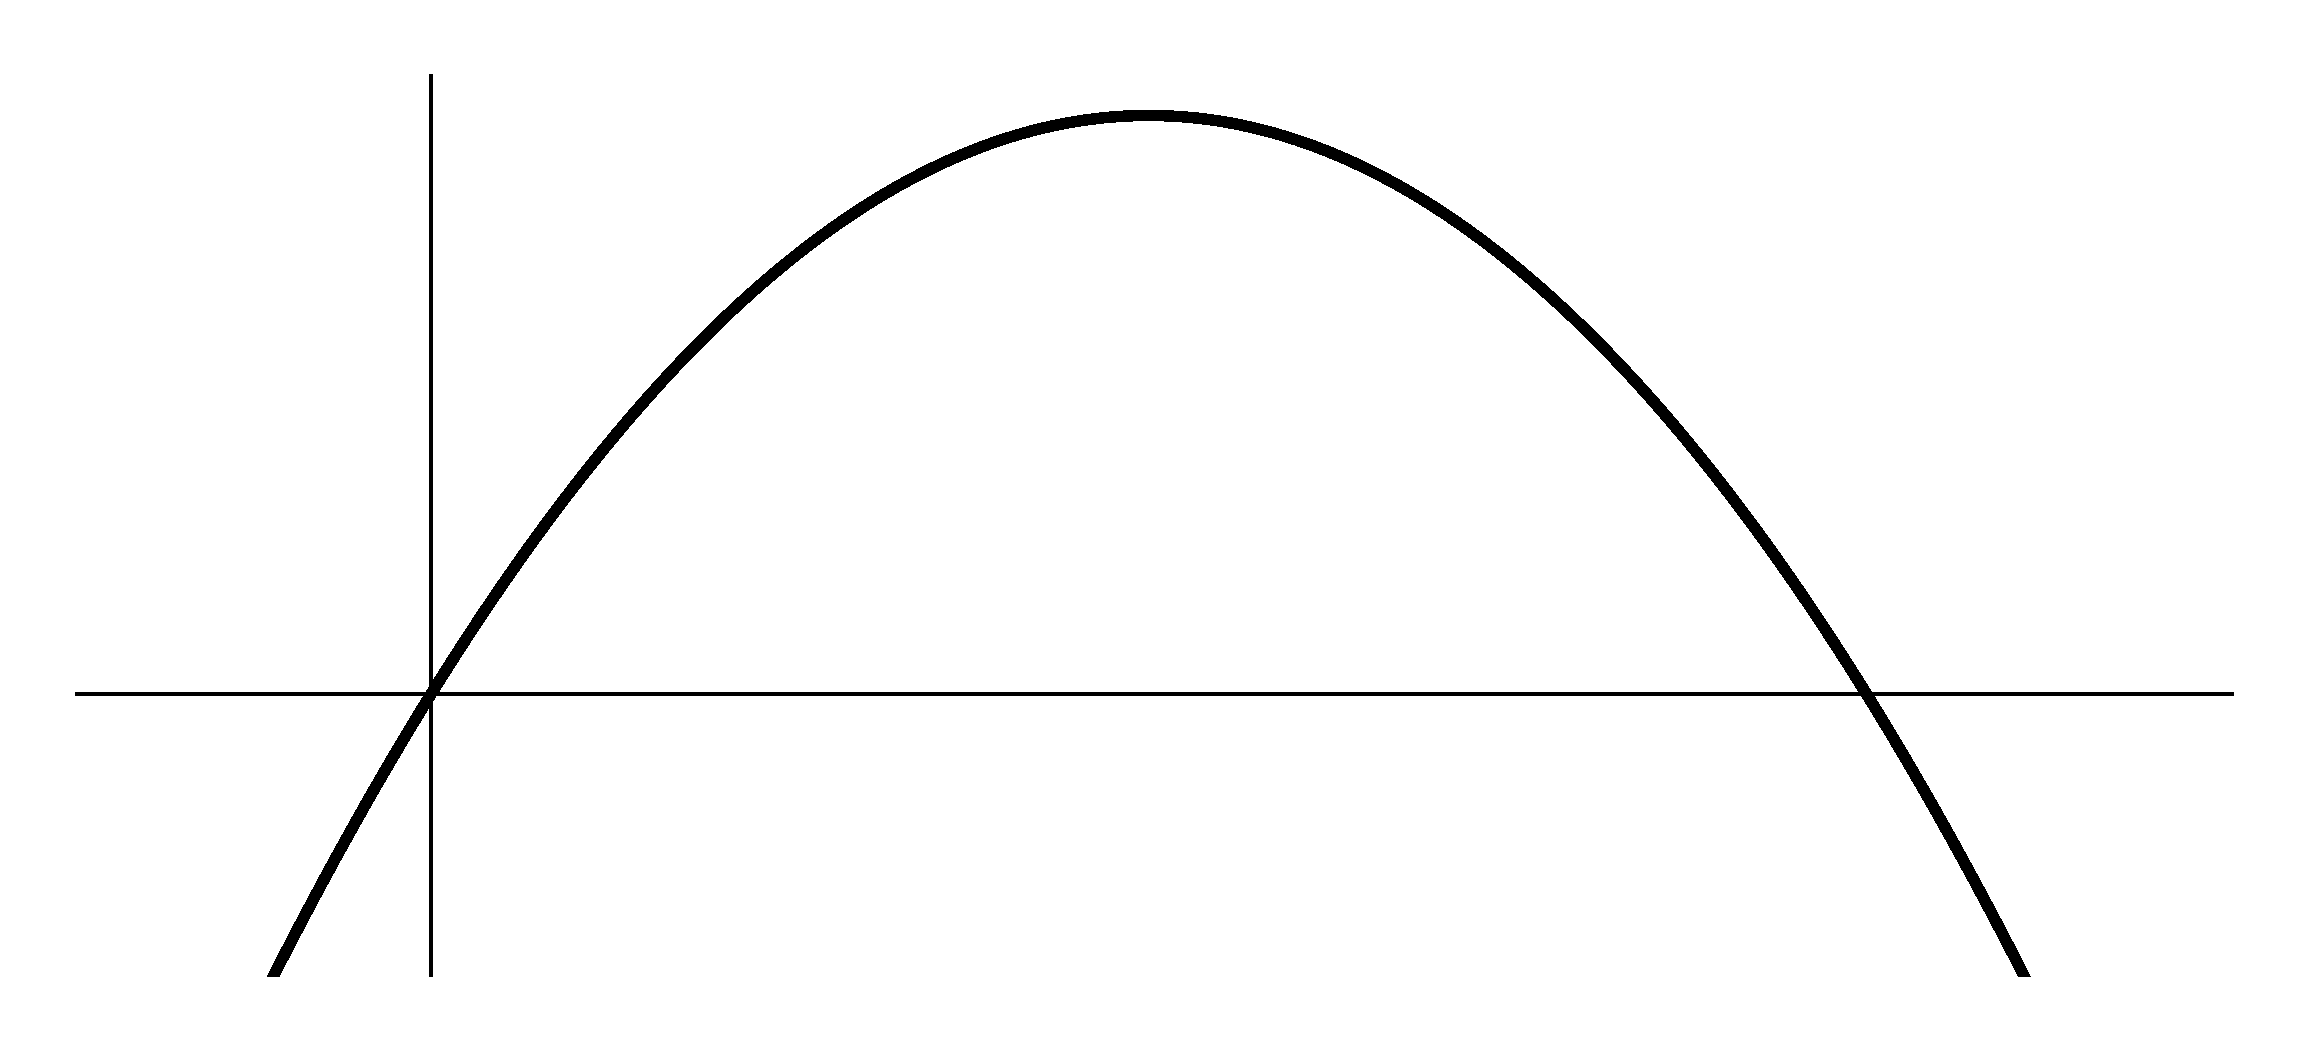
\includegraphics[width=5in]{01/01ValeriaGraph.pdf}
\end{center}

\item  Suppose two students are memorizing the elements on a list according to the rate of change equation \[\frac{dL}{dt}=0.5(1-L),\] where $L$ represents the fraction of the list that is memorized at any time $t$.
\begin{enumerate}
\item	If one of the students knows one-third of the list at time $t = 0$ and the other student knows none of the list, which student is learning most rapidly at this instant? Why?
\item	What does the rate of change equation predict for someone who begins with the list completely memorized? Explain.
\item	Suppose now that the list so long that no one can read it in a lifetime, like the decimal representation for $\pi$. In reality no one can memorize all the digits to $\pi$, but what does the rate of change equation predict will happen for a person who starts out not knowing any of the digits? That is, according to the rate of change equation, if $L = 0$ at time $t = 0$, is there ever a value of $t$ for which $L = 1$? Explain. 

\end{enumerate}

\item The letter $y$ appears in two places in the differential equation $ \displaystyle \frac{dy}{dt} = 0.3y.$
Is it appropriate to think of both occurrences of $y$ as function of $t$? Explain.


\item In algebra, the goal of solving an equation such as $x^2 + 4x =2$ is to find the values of $x$ that make a true statement. In differential equations, what is the goal of solving an equation such as $\displaystyle\frac{dx}{dt}+4x=2$? 

\item  For the differential equation   $\displaystyle \frac{dy}{dt}=1-y^2$,
\begin{enumerate}
\item	Sketch a slope field by hand. 
\item	Describe any shortcuts or patterns you used to make the task easier.
\item	Sketch several $y(t)$ graphs.
\end{enumerate}

\item Differential equations are often referred to as mathematical models. Explain what the phrase ``mathematical model'' means to you, what previous experiences you have had with mathematical models, and how the mathematical use of the word model is similar to and/or different from the everyday use of the word model ({\em e.g.}, fashion model, model airplane, model student).

\item Consider the differential equation
\[
\frac{dy}{dt}+ty=e^{-\frac{1}{2}t^2}; \quad y(0)=1
\]
Is $y(t)=te^{-\frac{1}{2}t^2}+e^{-\frac{1}{2}t^2}$ a solution?

\item
\begin{enumerate}
\item Go to the glossary and identify all terms that are relevant to this unit and list those terms here.
\item Are there other vocabulary terms that you think are relevant for this unit that were not included? If yes, list them.
\end{enumerate}



\end{enumerate}


%UNIT 2: A NUMERICAL APPROACH
%%%%%%%%%%%%%%%%%%%%%%%%%%%
%%%% Put the following at the top of each .tex file  %
\pagestyle{fancy}
\renewcommand{\theUnit}{2}
\ifthenelse{\isundefined{\UnitPageNumbers}}{}{\setcounter{page}{1}}
\rhead{Unit \theUnit: A Numerical Approach}
\lhead{
\includegraphics[width=1.25cm]{IODE-logo.png}}
\rfoot{\mypage}
\lfoot{}
\cfoot{}
\fancypagestyle{firstfooter}{\footskip = 50pt}
\renewcommand{\footrulewidth}{.4pt}
%%%%%%%%%%%%%%%%%%%%%%%%%%%
\vspace*{-20pt} \thispagestyle{firstfooter}
\pagebegin{A Rate of Change Equation for Limited Resources}

In a previous problem we saw that the rate of change equation $\displaystyle\frac{dP}{dt}=0.3P$ can be used to model a situation where there is one species, continuous reproduction, and unlimited resources. In most situations, however, the resources are not unlimited, so to improve the model one has to modify the rate of change equation $\displaystyle\frac{dP}{dt}=0.3P$ to account for the fact that resources are limited. 
\begin{enumerate}
\item	\label{02problem1}
\begin{enumerate}
\item In what ways does the modified rate of change equation \label{02problem1parta}
\[ \frac{dP}{dt}=0.3P\left(1-\frac{P}{10}\right) \] account for limited resources? (Think of 10 as scaled to mean 10,000 or 100,000) 
\vfill
\item	How do you interpret the solution with initial condition $P(0) = 10$? \label{02problem1partb}
\vfill
\item	Open the Slope Field Viewer, \href{https://ggbm.at/ZGeeGQbp}{\underline{https://ggbm.at/ZGeeGQbp}},
and plot the slope field for \[ \frac{dP}{dt}=0.3P\left(1-\frac{P}{10}\right). \]
(Note: In the Slope Field Viewer you will need to use the variable $y$ instead of $P$, and you may want to change the viewing window using the button on the right of the applet.) In what ways are your responses to parts \ref{02problem1parta} and \ref{02problem1partb} visible in the slope field? \label{02problem1partc}

\vspace{-1in}\hspace{-0.75in}
\includegraphics[width=0.5in]{02/02SlopeFieldViewerQR.png}
\vfill

\item	In this problem, negative $P$ values do not make sense, but we can still mathematically make sense of the slope field for negative $P$ values. Explain why the slope field looks the way it does below the $t$-axis. \label{02problem1partd}
\vfill
\end{enumerate}

\item If there are initially $P(0)=2$ fish in the lake, approximately how many fish are in the lake at time $t=2$?  How did you arrive at your approximation? (Hint: Initially $\frac{dP}{dt} = 0.48$, but what meaning does $0.48$ have?) \label{02problem2}
\vfill
\end{enumerate}

\clearpage
%%%%%%%%%%%%%%%%%%%%%%%%%%%%%%%%%%%
\pagebegin{Using a Slope Field to Predict Future Fish Populations}

Below is a slope field for the rate of change equation $\displaystyle \frac{dP}{dt}=0.3P\left(1-\frac{P}{10}\right).$ 
\begin{center}
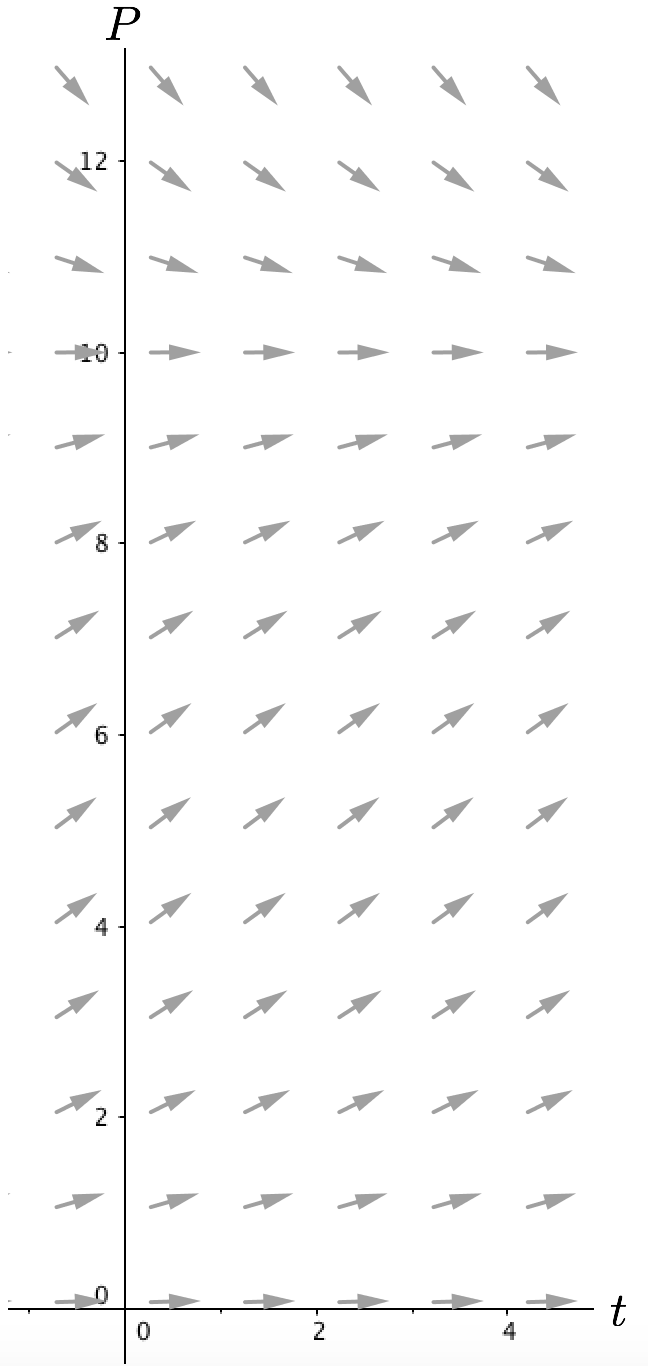
\includegraphics[width=2in]{02/02SlopeFieldFish.png}
\end{center}
 
\begin{enumerate}[resume]
\item \label{02problem2}
\begin{enumerate}
\item On the slope field above, stitch together in a tip to tail manner several tangent vectors to produce a graph of the population versus time if at time $t = 0$ we know there are 8 fish in the lake (again, think of 8 as scaled for say, 8000 or 80,000). \label{02problem3parta}
\vs
\item Reproduce your technique as much as possible using the Slope Field Stitcher applet, \\ \href{https://ggbm.at/FZn4WHeU}{\underline{https://ggbm.at/FZn4WHeU}}.  You can use the arrow buttons to move the initial vector around, and then create subsequent vectors to stitch on using the appropriate button. \label{02problem3partb}

\vspace{-.3in}\hspace{-0.75in}
\includegraphics[width=0.5in]{02/02SlopeFieldStitcherQR.png}
\end{enumerate}

\item	Explain how you are thinking about rate of change \textbf{in your method}. For example, is the rate of change constant over some increment? If yes, over what increment? If no, is the rate of change always changing? \label{02problem4}
\vfill

\clearpage

\item Using the differential equation $\displaystyle\frac{dP}{dt}=P\left(1-\frac{P}{20}\right)$ and initial condition $P(0) = 10$, Jos{\'e} and Julie started the following table to numerically keep track of their tip-to-tail method for connecting tangent vectors. Explain Jos{\'e}'s and Julie's approach and complete their table. \textbf{Round to two decimal places.} \label{02problem5}

{
\renewcommand{\arraystretch}{1.5}
\newcolumntype{R}{>{\centering\arraybackslash}X}%
\begin{tabularx}{.4\textwidth}{ |R|R|R| }
\hline
$t$ & $P$ & $\frac{dP}{dt}$\\\hline
0 & 10 & 5\\\hline
0.5 & 12.5 & \\\hline
1.0&&\\\hline
1.5&&\\\hline
\end{tabularx}}
\vfill

\item	Using the same differential equation and initial condition as Jos{\'e} and Julie, Derrick and Delores started their table as shown below. Explain how Derrick and Delores' approach is different from Jos{\'e} and Julie's and then complete their table. \textbf{Round to two decimal places.} \label{02problem6}

{
$\displaystyle  \frac{dP}{dt}=P\left( 1-\frac{P}{20}\right) $
 
\renewcommand{\arraystretch}{1.5}
\newcolumntype{R}{>{\centering\arraybackslash}X}%
\begin{tabularx}{.4\textwidth}{ |R|R|R| }
\hline
$t$ & $P$ & $\frac{dP}{dt}$\\\hline
0 & 10 & 5\\\hline
.25 & 11.25 & \\\hline
.5&&\\\hline
.75&&\\\hline
\end{tabularx}}
\vfill

\item Which approach do you think is more accurate and why? \label{02problem7}
\vfill

\clearpage

\item
\begin{enumerate}
\item Consider the differential equation $\displaystyle\frac{dy}{dt}=y+t$ and initial condition $y(0) = 4$. Use Jos{\'e} and Julie's approach to find $y(1.5)$. Show your work graphically and in a table of values. \label{02problem8parta}
\vfill
\vfill
\item Is your value for $y(1.5)$ the exact value or an approximate value? Explain. \label{02problem8partb}
\vfill
\end{enumerate}
\item	\textbf{Generalizing your tip-to-tail approach}. Create an equation-based procedure/algorithm that would allow you to predict future $y$-values for any differential equation $\displaystyle\frac{dy}{dt}$, any given initial condition, and any time increment. \label{02problem9} \vfill \vfill

\end{enumerate}

\clearpage
%%%%%%%%%%%%%%%%%%%%%%%%%%%%%%%%%%%%%%%%%%%%%%
\pagebegin{Homework Set 2}
 \begin{enumerate}

\item A slope field for the differential equation $\displaystyle\frac{dy}{dt}=0.5(y+t)$ is shown below. \label{02HWproblem1}
\begin{center}
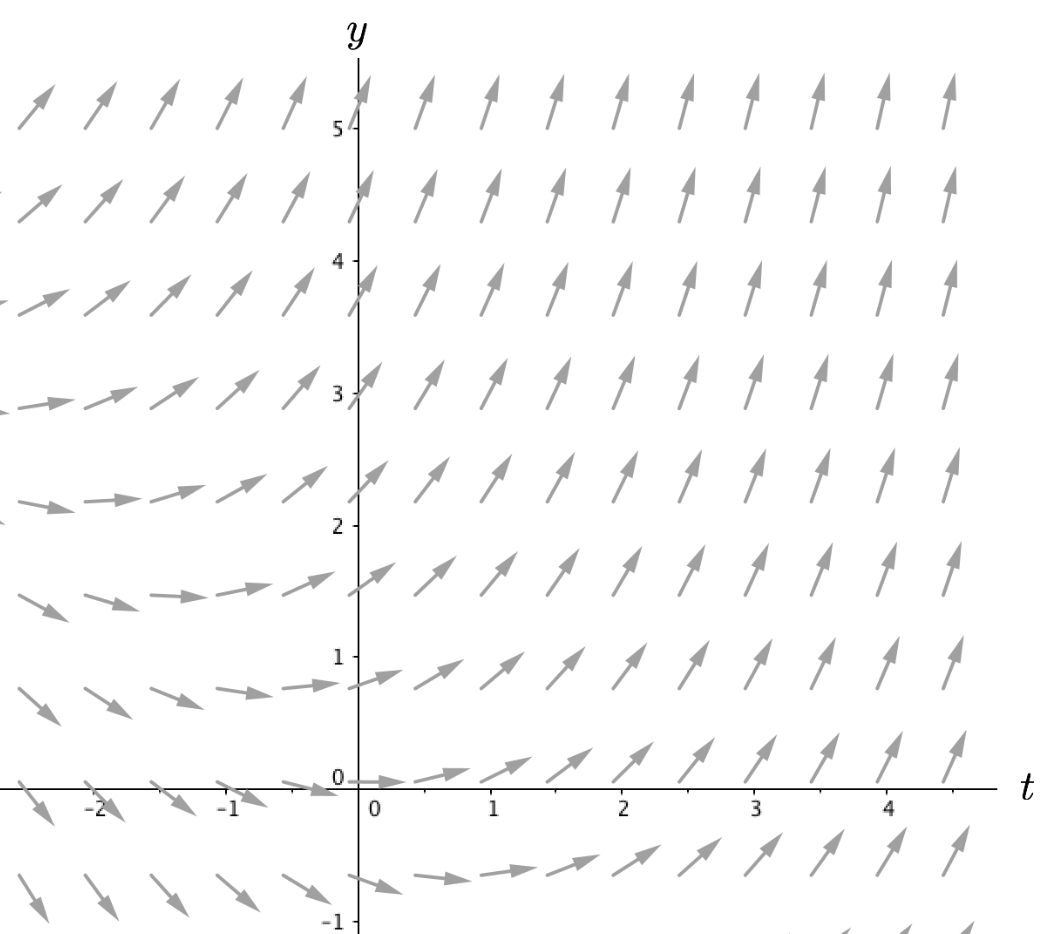
\includegraphics[width=6in]{02/02HWSlopeField1.png}
\end{center}
\begin{enumerate}
\item	For the initial condition of $y(0) = 1$, sketch on the above slope field what you think two iterations of the ``tip-to-tail'' method with a step size of 1 unit should look like. Do this \textbf{without} doing any computations. \label{02HWproblem1parta}
\item	Again, without doing any computations, sketch on the same slope field what you think three iterations with a step size of 0.5 units should look like for the same initial condition (perhaps using a different color). \label{02HWproblem1partb}
\item	Use the tip-to-tail ({\em i.e.}, Euler's) method to numerically compute approximations for parts \ref{02HWproblem1parta} and \ref{02HWproblem1partb} and then compare your graphical predictions to the numerical results. \label{02HWproblem1partc}
\end{enumerate}

\begin{comment}
\begin{hwsoln}
\begin{enumerate}
\item See picture.
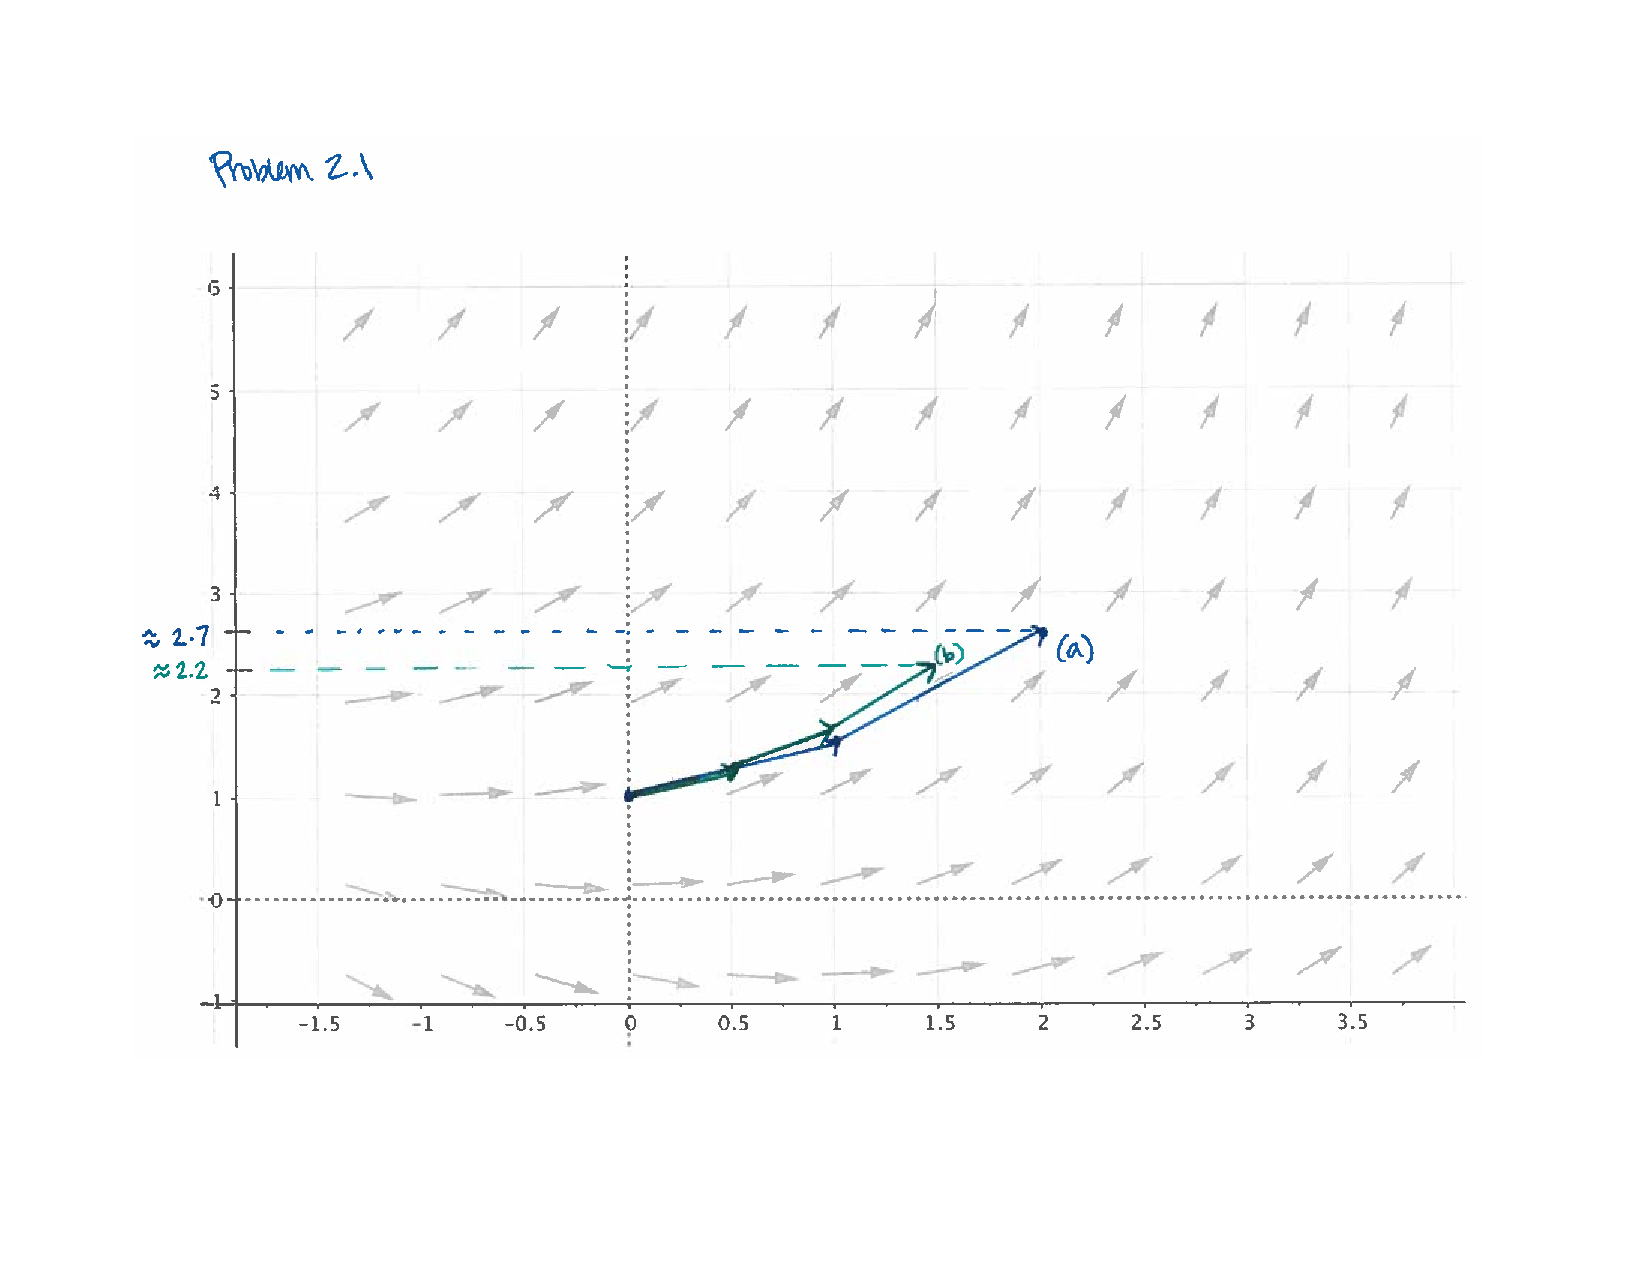
\includegraphics[width=4in]{02/02StitchOnMesoln.pdf}
\item See picture.
\item Given the initial condition $y(0) = 1$ and $\Delta t=1$, two steps of Euler's method gives the following:

$\frac{dy}{dt}\Big|_{t=0} = 0.5 (1+0) = \frac{1}{2} \quad \implies y(1)\approx y(0)+\frac{1}{2} = \frac{3}{2}  \\
\frac{dy}{dt}\Big|_{t=1} = 0.5 \left(\frac{3}{2}+1\right) = \left(\frac{1}{2}\right)\left(\frac{5}{2}\right) = \frac{5}{4} \quad \implies y(2)\approx y(1)+\frac{5}{4} = \frac{11}{4} = 2.75\\\textrm{(pretty close to the picture!)}$
\vs
Now using three iterations of Euler's method with $\Delta t=\frac{1}{2}$ we have:\\
$ \frac{dy}{dt}\Big|_{t=0} = 0.5 (1+0) = \frac{1}{2} \quad \implies y\left(\frac{1}{2}\right)\approx y(0)+\left(\frac{1}{2}\right)\left(\frac{1}{2}\right) = \frac{5}{4}  \\
\frac{dy}{dt}\Big|_{t=0.5} = 0.5 \left(\frac{5}{4}+\frac{1}{2}\right)  = \frac{7}{8} \quad \implies y(1)\approx y\left(\frac{1}{2}\right)+\frac{1}{2}\left(\frac{7}{8}\right)= \frac{5}{4}+\frac{7}{16} = \frac{27}{16}\\
\frac{dy}{dt}\Big|_{t=1} = 0.5 \left(\frac{27}{16}+1\right)  = \frac{43}{32} \quad \implies y\left( \frac{3}{2} \right)\approx y(1)+\frac{1}{2}\left(\frac{43}{32}\right) = \frac{27}{16} +\frac{43}{64}= 2.36$\\
(again, pretty close to the picture!)

\end{enumerate}
\end{hwsoln}
\end{comment}

\clearpage

\item Consider a differential equation with the given slope field and the initial value $y(0)=1$. \label{02HWproblem2}
\begin{center}
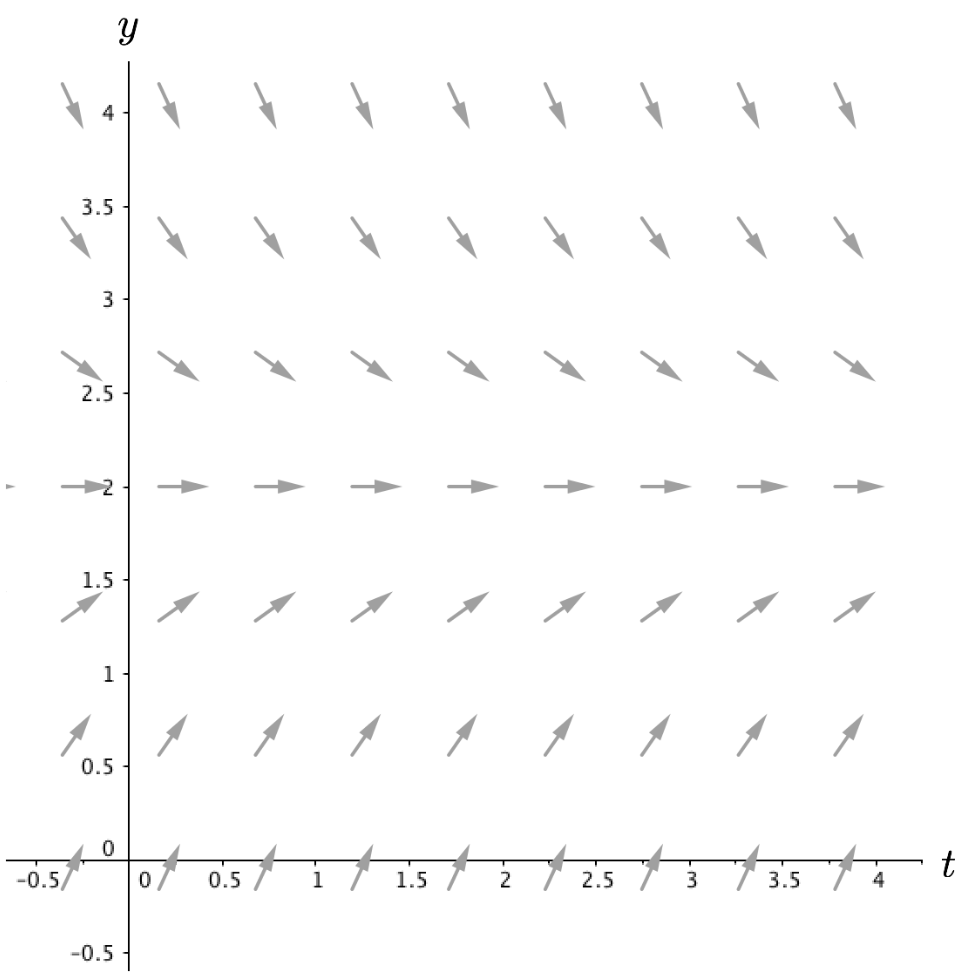
\includegraphics[width=5in]{02/02HWSlopeField2.png}
\end{center}
\begin{enumerate}
\item Explain why, if you wanted to approximate $y(2)$ using two steps of Euler's method, you would need $\Delta t = 1$.  \label{02HWproblem2parta}
\item Use a straight edge to graph two steps of Euler's method to approximate $y(2)$. \label{02HWproblem2partb}
\item This time, instead of using two steps of Euler's method, sketch on the same slope field what it would look like if you used four steps of Euler's method to approximate $y(2)$. \label{02HWproblem2partc}
\item Besides the obvious difference that the step size is different, state two other things that are different between your answers to parts \ref{02HWproblem2partb} and \ref{02HWproblem2partc}. \label{02HWproblem2partd}
\item Besides the obvious fact that they both use Euler's method, what is similar about the first step to your answers to parts \ref{02HWproblem2partb} and \ref{02HWproblem2partc}? \label{02HWproblem2parte}

\end{enumerate}

\begin{comment}
\begin{hwsoln}
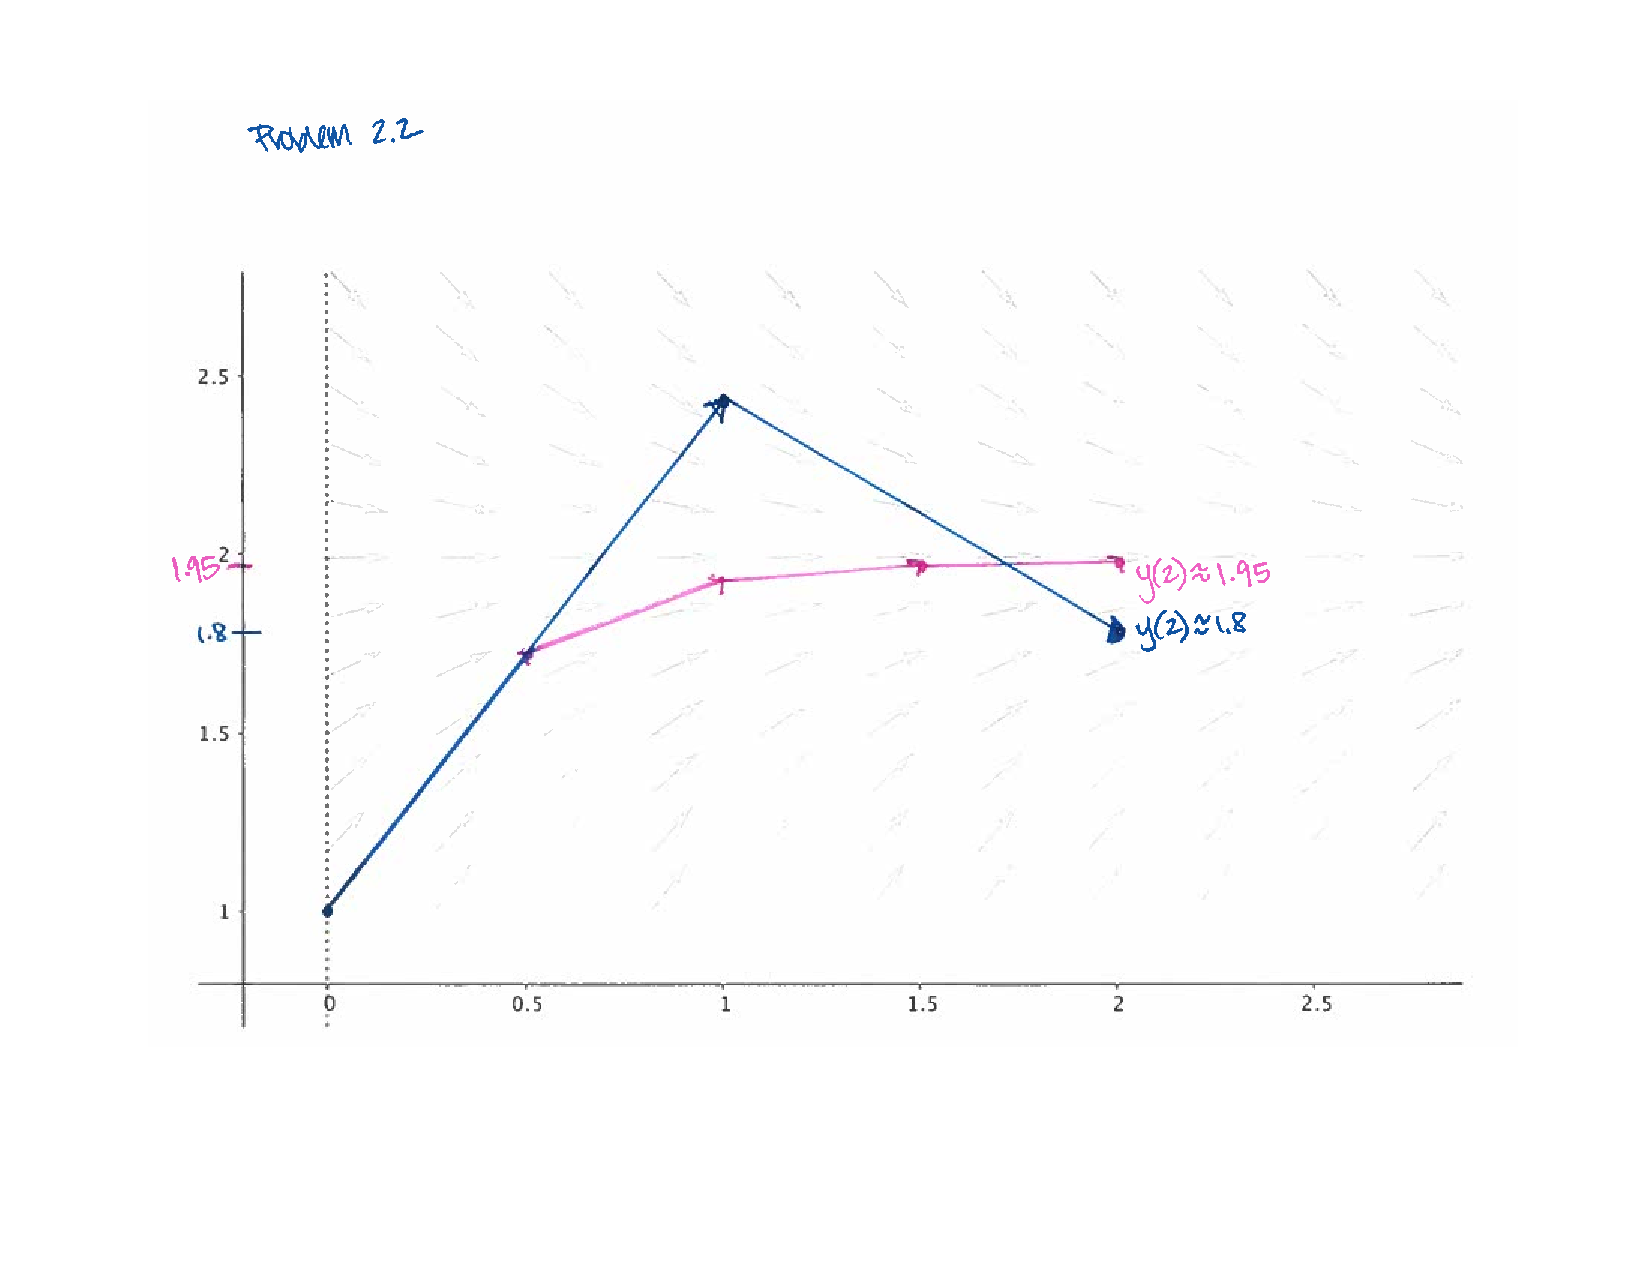
\includegraphics[width=4in]{02/02Eulergraphicalsoln}
\begin{enumerate}
\item See picture (blue).  $y(2)\approx 1.8$.
\item See picture (pink).  $y(2)\approx 1.95$.
\item The larger step size is almost certainly less accurate (or will be in most cases) because it assumes a constant slope for a longer period of time despite the actual solution having a constantly changing slope.  Plus, the larger step size ends up using approximate $y$-values on either side of the constant solution $y=2$, and crosses over this line during Euler's method, which wouldn't be true of an exact solution curve.  The smaller step size solution here ``looks'' more like what we'd expect of an exact solution. {\em (Keep in mind the students still don't know about Uniqueness, officially, so it's okay if this reasoning is a bit vague or incomplete.)}
\item These solutions are similar in the fact that they're both just approximations, and they both end up producing approximate $y$-values less than 2.
\end{enumerate}
\end{hwsoln}
\end{comment}

\clearpage

\item	Suppose we have a rate of change equation and initial condition for the population of raccoons in Lake County. Below is a graph of an \textbf{exact} solution. \label{02HWproblem3}

\begin{center}
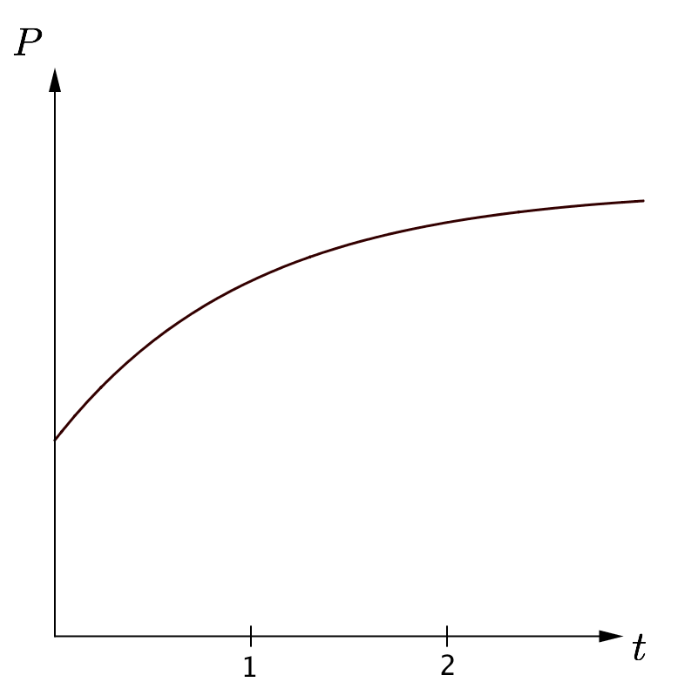
\includegraphics[width=2in]{02/02HWLotRExact.png}
\end{center}

Merry, Pippin, and Sam attempted to use the ``tip-to-tail'' Euler method to predict what the population of raccoons would be at time $t = 2$, with time increments one unit.  However, they arrived at different graphs for their predictions.  Their predictions are given below, and are shown with the exact solution.

\begin{tabular}{ccc}
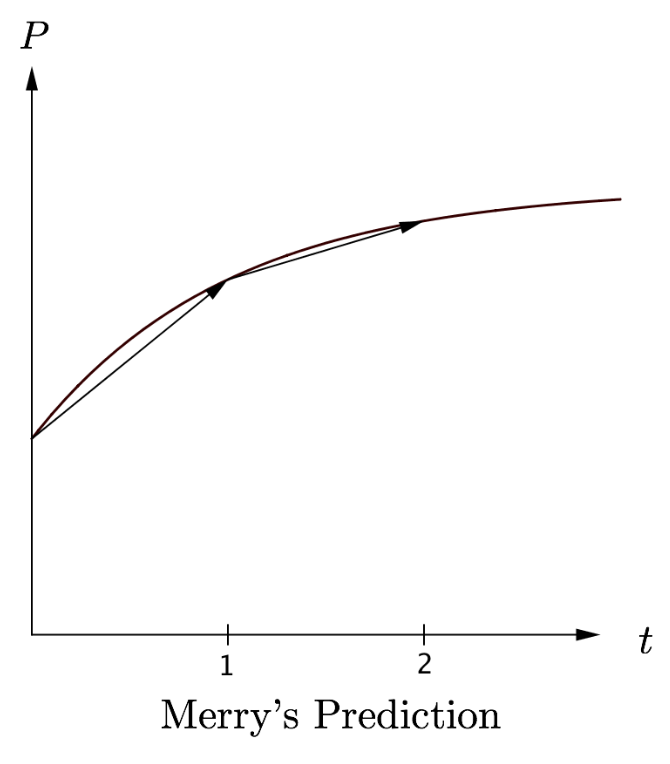
\includegraphics[width=2in]{02/02HWLotRMerry.png} & 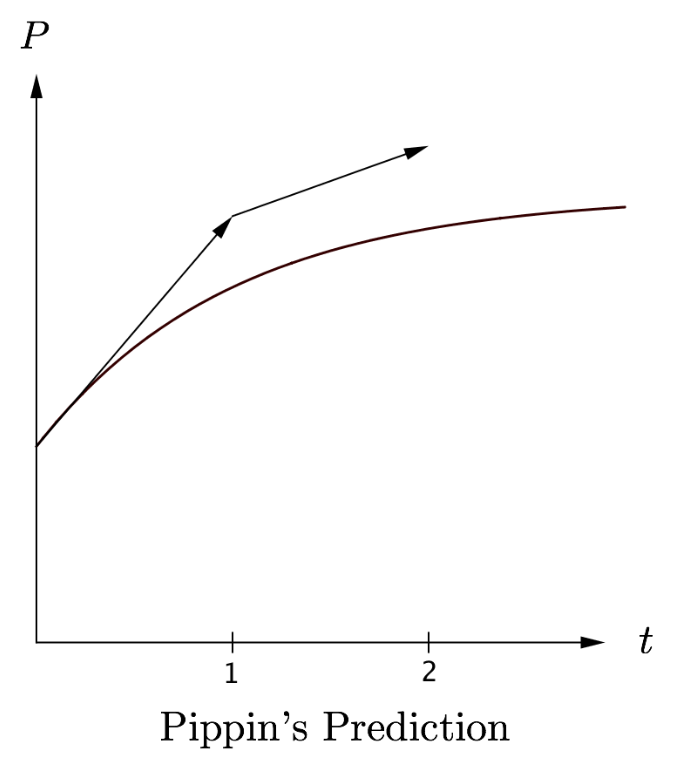
\includegraphics[width=2in]{02/02HWLotRPippin.png} & 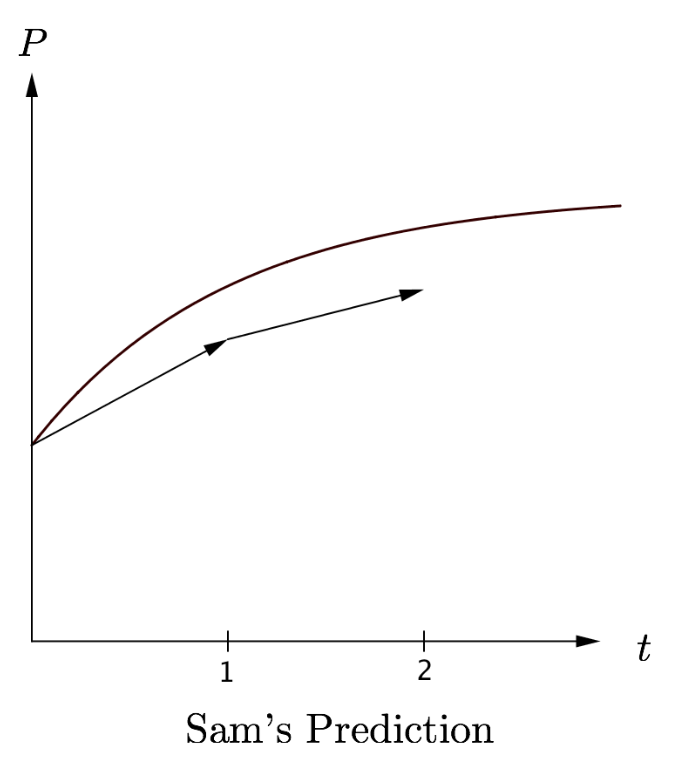
\includegraphics[width=2in]{02/02HWLotRSam.png}\\
\end{tabular}

For each prediction, give reasons as to whether or not each person illustrated the correct relationship between Euler's method and the exact solution. 

\item Suppose the function $y(t) = 6t +1$ is a solution to a particular differential equation. For the initial condition $y(0) = 1$, is a graph of the tip-to-tail Euler method exactly the same as the graph of the exact solution? Does your response depend on step size? Explain. \label{02HWproblem4}



\item Compute by hand four steps of the tip-to-tail Euler method for the differential equation $\displaystyle\frac{dy}{dt}=y-t$  with initial condition $y(0) = 2$ and step size 0.5. \label{02HWproblem5}

\newpage

\item \textbf{Euler's Method Using a Spreadsheet.} Learning to use a spread sheet for various applications in engineering and mathematics is a valuable skill. Your task in this problem is to use Excel to generate as many steps of the Euler method that you want. \textit{If you are already familiar with Excel, skip the example below and go directly to part a}. \label{02HWproblem6}

EXAMPLE:  Here are step by step instructions for how to use Excel to generate 15 steps of the algorithm   $Y_{\textrm{next}} = 2 \cdot Y_{\textrm{now}} + 1$ with initial condition $Y = 3$. 

\begin{itemize}
\item	Open an Excel workbook 
\item	Select cell A1 by clicking on the cell in this location and type in Ynow as a column heading
\item	Select cell B1 and create a column heading called Ynext
\item	Select cell A2 and type in the number 3 (this is the given initial Y-value)
\item	Select cell B2 and type =2*A2+1 (after pressing Enter the number 7 will appear in this cell)
\item	Select cell A3 and type =B2
\item	Select and copy cell B2  (An animated dashed-line will appear around the cell)
\item	Select cells B3 through B15 and paste 
\item	Select and copy cell A3
\item	Select cells A4 through A15 and paste
\item	Do a few hand computations to verify the results

\end{itemize}
\begin{enumerate}
\item	Using a step size $\Delta t$ of your choice, figure out how to use Excel to generate at least 20 steps for Euler's method, $\displaystyle y_{\textrm{next}} = y_{\textrm{now}} + (\frac{dy}{dt})_{now}\cdot\Delta t$, for the differential equation $\displaystyle\frac{dy}{dt}=0.3y(1-\frac{y}{12.5})$ with initial condition $y(0) = 3$. In order to make it easier to graph the results, make your first column $t_{\textrm{now}}$ and your second column $y_{\textrm{now}}$. Turn in a print out your results and verify the first three steps by hand. \label{02HWproblem6parta}

\item	Use the Chart Wizard scatter plot option to create a graph of your $(t, y)$ data from part \ref{02HWproblem6parta}. An easy way to do this is to first highlight all the data in the $t_{\textrm{now}}$ and $y_{\textrm{now}}$ columns, select Chart Wizard, and follow the prompts. Turn in a print out of your results. \label{02HWproblem6partb}
\end{enumerate}

\begin{comment}
\begin{hwsoln}
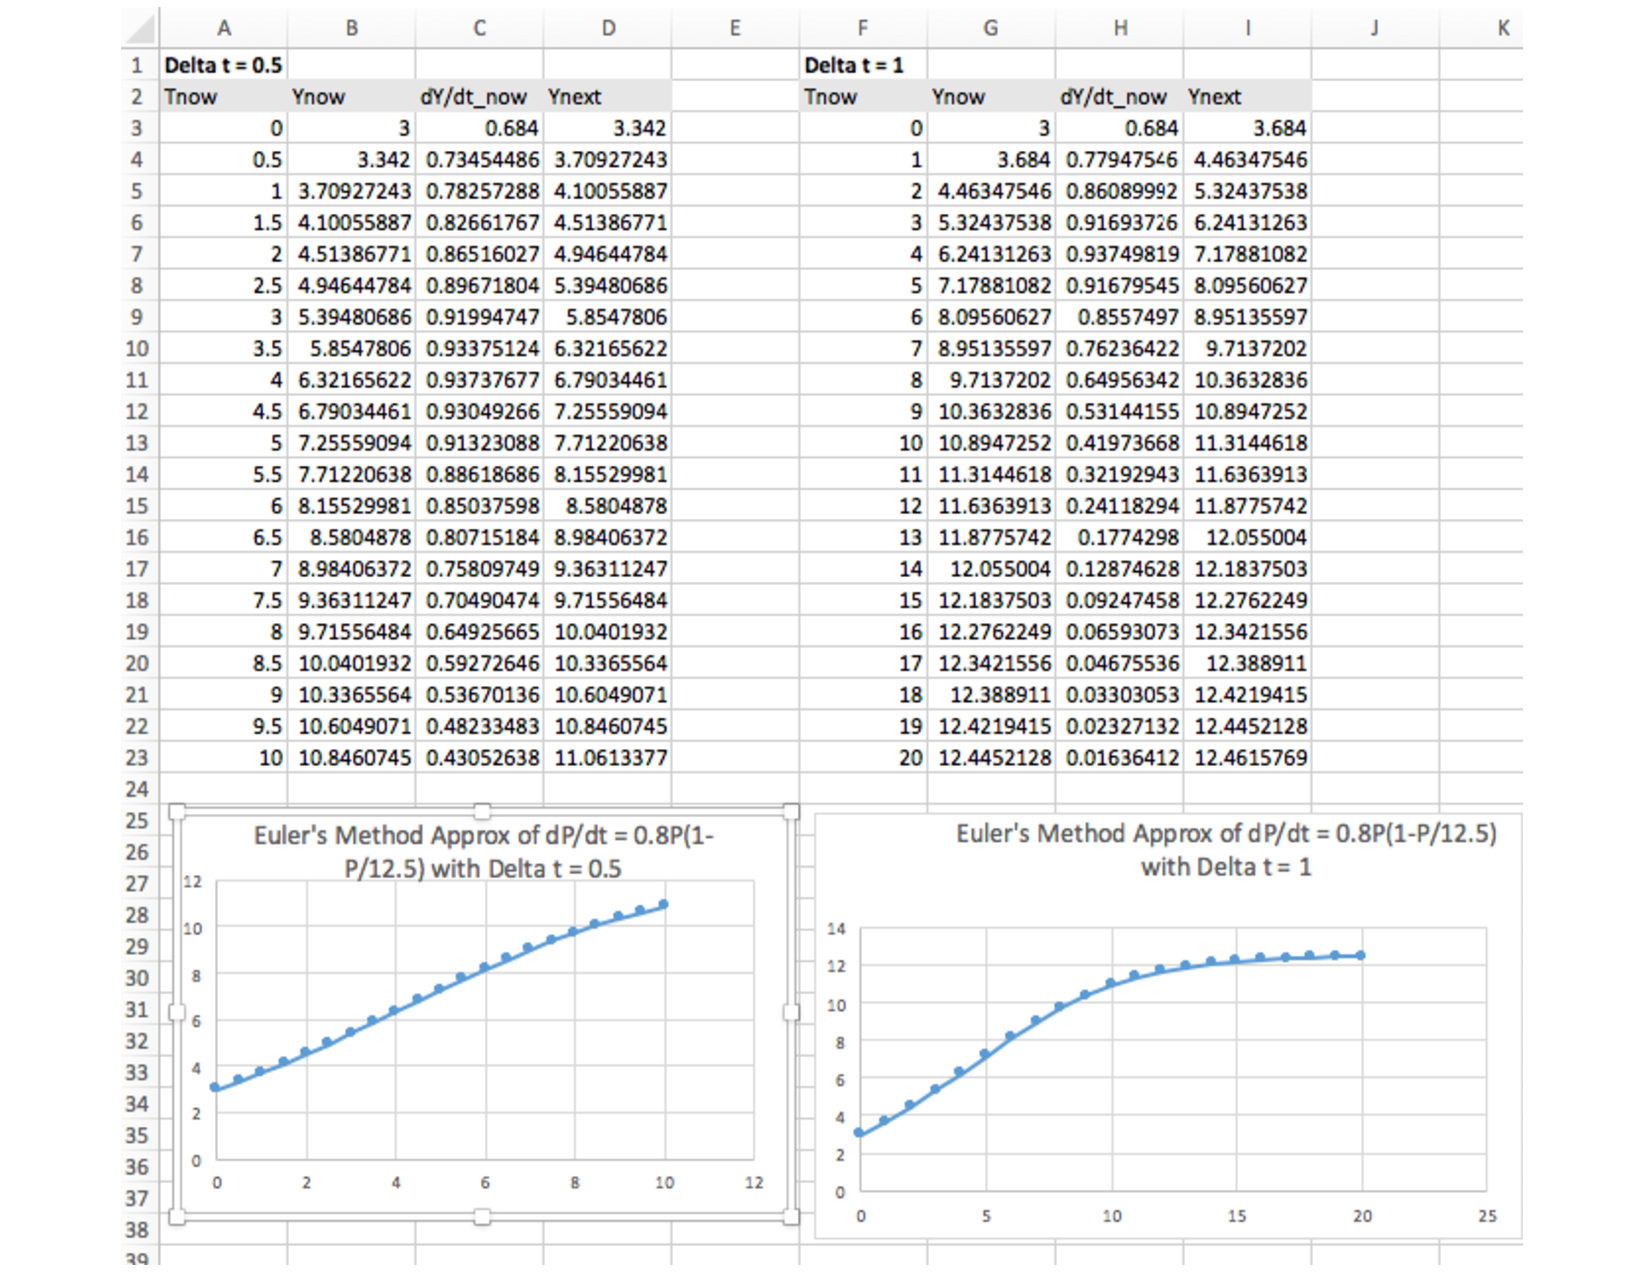
\includegraphics[width=5in]{02/02Eulerexcel.pdf}
\end{hwsoln}
\end{comment}

\item	Two students are having a discussion about the equal sign in the rate of change equation $\displaystyle\frac{dP}{dt} = 0.5P\left(1 - \frac{P}{100}\right)$. One student says he thinks about the equal sign as instructions for calculating. The other student says he thinks about the equal sign as a kind of mirror. How do you think about the equal sign in a rate of change equation? \label{02HWproblem7}

\clearpage

\item A group of scientists created the differential equation $\displaystyle\frac{dP}{dt}=0.8P\left(1-\frac{P}{5}\right)$  to predict future fish populations in Lake Minnetonka, where $P$ represents thousands of fish and $t$ is in years. \label{02HWproblem8}

\begin{enumerate}
\item	If you were to plot a slope field for this rate of change equation, what window for the $P$ and $t$ values would you use to make sure the most important features are clearly shown? Explain. \label{02HWproblem8parta}
\item	What does this rate of change equation predict about the long-term outcome of the fish population if the initial population is 2 ({\em i.e.}, $P = 2$ at $t = 0$)? How about if $P = 6$ at $t = 0$? \label{02HWproblem8partb}
\item	Why are the predictions you made in part \ref{02HWproblem8partb} reasonable (or not) for a fish population? Explain. \label{02HWproblem8partc}
\item	Carry out by hand three steps of Euler's method with a step size of 0.5 for the initial condition $P(0) = 5$. \label{02HWproblem8partd}
\end{enumerate}

\item
\begin{enumerate}
\item Go to the glossary and identify all terms that are relevant to this unit and list those terms here.
\item Are there other vocabulary terms that you think are relevant for this unit that were not included? If yes, list them.
\end{enumerate}

\end{enumerate}

%UNIT 3: AN ANALYTIC APPROACH
%%%%%%%%%%%%%%%%%%%%%%%%%%%
%%%% Put the following at the top of each .tex file  %
\pagestyle{fancy}
\renewcommand{\theUnit}{3}
\ifthenelse{\isundefined{\UnitPageNumbers}}{}{\setcounter{page}{1}}
\rhead{Unit \theUnit: An Analytic Approach}
\lhead{
\includegraphics[width=1.25cm]{IODE-logo.png}}
\rfoot{\mypage}
\lfoot{}
\cfoot{}
\fancypagestyle{firstfooter}{\footskip = 50pt}
\renewcommand{\footrulewidth}{.4pt}
%%%%%%%%%%%%%%%%%%%%%%%%%%%
\vspace*{-20pt} \thispagestyle{firstfooter}
\pagebegin{Comparing Predictions}

Jerry and Tom are using the differential equation $\displaystyle\frac{dP}{dt} = 0.2P$ to make predictions about the number of a particular species of fish in Lake Michigan. They know that the initial population $P$ is 2 at time $t = 0$ (as before, think of 2 as scaled for say, 2,000 or 20,000).
 \vs
Although Jerry and Tom have the same goal (to obtain predictions for future fish population), they have different approaches to achieve this goal. 

\begin{itemize}
\item	Tom's approach is to create a graph of the number of fish versus time by connecting slope vectors tip-to-tail, where the rate of change is constant over some time interval, for example $\Delta t=0.5$. 
\item Jerry's approach is to create a graph of the number of fish versus time by using a continuously changing rate of change. 

\end{itemize}
\begin{enumerate}

\item Sketch Tom and Jerry's approaches below. Will these two approaches result in the same predictions for the number of fish in, say, $2.5$ years? If yes, why? If not, how and why will the graphs of their approaches be different?\label{03problem1}
\begin{center}
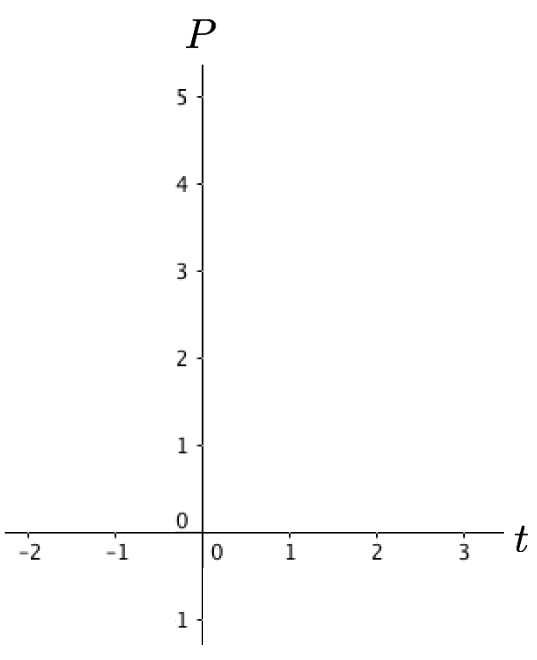
\includegraphics[width=3in]{03/03TomJerry.png}
\end{center}
\end{enumerate}
\clearpage

%%%%%%%%%%%%%%%%%%%%%%
\pagebegin{Separation of Variables}

\begin{enumerate}[resume]
\item	\textbf{Finding the exact solution}. Jerry's approach involves using a continuously changing rate of change, which corresponds to finding an ``exact solution.'' \label{03problem2}
\begin{enumerate}

\item	Why do you think the phrase ``exact solution'' is used to describe the result of Jerry's approach? Explain why it is appropriate to describe the result of Tom's approach as an ``approximate solution''. \label{03problem2parta}

\vfill
\item Use the chain rule to write down, symbolically, the derivative with respect to $t$ of $\ln (P)$, where $P$ is shorthand for $P(t)$. \label{03problem2partb}
\end{enumerate}
\vfill

\clearpage

Next you will learn a technique for finding the exact solution corresponding to Jerry's approach. We begin by considering the chain rule.

\begin{enumerate}[resume]
\item	 The following is a method to find the analytic solution to $\displaystyle\frac{dP}{dt}= 0.2P$. For now assume that $P > 0$. This assumption corresponds to the population growth context and it will make the algebra easier and hence the underlying idea clearer.  \label{03problem2partc}
 
\end{enumerate}

\begin{center} \renewcommand{\arraystretch}{1.5}
\newcolumntype{V}{>{\centering\arraybackslash} m{.5\linewidth} }
\begin{tabular}{|p{2in}|V|}
\hline

Divide both sides of \newline $\frac{dP}{dt}=0.2P$ by $P$ &
{} \\
{} & {} \\
\hline

Replace $\frac{1}{P}\frac{dP}{dt}$ with $\left[ \ln(P)\right]'$ & 
{} \\
{} & {} \\
\hline
	 
Write integrals with respect to $t$ on both sides & 
\\{} & {} \\ 
\hline
	 
Apply the Fundamental Theorem of Calculus to integrate both sides & 
\\{} & {} \\
\hline	 

Solve for $P$ (and remember that $P$ is actually a function, $P(t)$) & 
\\{} & {} \\
\hline

Show that $P$ can be written as $P(t) = ke^{0.2t}$ & 
\\{} & {} \\
{} & {} \\
\hline
\end{tabular} \end{center}

The end result, $\displaystyle P(t)=ke^{0.2t}$ is called the \textbf{general solution} because it represents all possible functions that satisfy the differential equation. We can use the general solution to find any \textbf{particular solution}, which is a solution that corresponds to a given initial condition.

\item	Use the same technique to find the general solution to $\displaystyle\frac{dy}{dt}=\frac{t}{3y^2}$. The first step is done for you. \label{03problem3}
\vs
$\displaystyle 3y^2\frac{dy}{dt}=t$
\vfill

\clearpage

\item In practice, we often circumvent explicit use of the chain rule and instead use a shortcut to more efficiently find the general solution. The shortcut involves treating the derivative $\frac{dP}{dt}$ as a ratio and ``separating'' the $dP$ and $dt$. In the table below, follow the instructions to see how the shortcut works, using again the equation $\displaystyle\frac{dP}{dt} = 0.2P$. (See \href{http://kevinboone.me/separation_variables.html}{\underline{http://kevinboone.me/separation\textunderscore variables.html}}) for a nice explanation of the shortcut). \label{03problem4}
\vs

\begin{center}\renewcommand{\arraystretch}{1.5}
\newcolumntype{V}{>{\centering\arraybackslash} m{.5\linewidth} }
\begin{tabular}{|p{2.5in}|V|}
\hline
`Separate' the $dP$ from the $dt$ so that $dP$ and $P$ are on the same side. (If there are $t$'s in the equation they must go on the same side as $dt$.)
	  &
{} \\\hline

Integrate both sides of the equation (one side with respect to $P$, the other with respect to $t$)	  &
{} \\\hline

Continue as before to arrive at a solution of the form $P(t)=\underline{\hskip1cm}$	 	  &
{} \\
{} & {} \\
{} & {} \\
{} & {} \\
{} & {} \\
{} & {} \\
{} & {} \\
{} & {} \\ \hline
\end{tabular}
\end{center}

\item	Use the shortcut to find the general solution to  $\displaystyle \frac{dy}{dt}=\frac{t}{3y^2}$. \label{03problem5}
\vfill

\clearpage

\item	A differential equation together with an initial condition is called an \textbf{Initial Value Problem} (IVP). To solve an IVP one first must find the general solution and then use the initial condition to find the particular solution corresponding to the initial condition. \label{03problem6} \\ Solve the following IVP:    
\[ \frac{dy}{dt}=\frac{t}{y}\hspace{0.5in} y(2)=-1\]
\vfill

\begin{enumerate}
\item	 For what values of $t$ is your solution valid? Why? \label{03problem6parta} 
\vskip1cm

\item Check to see that your {particular} solution ``fits'' the differential equation by substituting the solution and its derivative into the original differential equation. \label{03problem6partb} 
\vfill

\item	Use the GeoGebra applet, \href{https://ggbm.at/SbHk2n4H}{\underline{https://ggbm.at/SbHk2n4H}}, to check to see that your specific solution ``fits'' the differential equation by plotting the slope field and then plotting the graph of the solution on top of the slope field. Explain how this relates to Jerry's approach. \label{03problem6partc}

\vspace{-.25in}\hspace{-.75in}
\includegraphics[width=0.5in]{03/03IVPQR.png}
\vfill

\item Consider a different initial condition, $y(2) = 0$, to the same differential equation, $\displaystyle\frac{dy}{dt}=\frac{t}{y}$. Note that even though $\displaystyle\frac{dy}{dt}$ is undefined when $y = 0$, our separation of variables technique can still yield something meaningful. What should the solution to this IVP be? \label{03problem6partd} 
\vfill
\end{enumerate}

\end{enumerate}

\clearpage

%%%%%%%%%%%%%%%%%%
\pagebegin{Making Connections}

\begin{enumerate}[resume]
\item For the first slope field for $\frac{dL}{dt} = 0.5(1 - L)$ on the following page,\label{03problem7}
\begin{enumerate}

\item	Using Jerry's approach, sketch as accurately as possible a graph of the solution with initial condition $L(0) = 1/3$. \label{03problem7parta}
\item	Make a copy of this sketch on a transparency. \label{03problem7partb}
\item	If you wanted to obtain the graph of the solution with initial condition $L(0) = 1/2$, how, if at all, might you move the copy of your graph with initial value 1/3 so that it is now a graph of the solution with initial value 1/2? What feature of the differential equation justifies your approach? \label{03problem7partc}
\item	Find the general solution for $\displaystyle\frac{dL}{dt}= 0.5(1-L)$ and explain how your results from part \ref{03problem7partc} can be understood from the general solution.\label{03problem7partd}
\vfill	

\end{enumerate}
\item	For the second slope field for $\frac{dh}{dt} = -t + 1$ on the following page,\label{03problem8}
\begin{enumerate}
\item	Using Jerry's approach, sketch as accurately as possible a graph of the solution with initial condition $h(0) = 1/2$. \label{03problem8parta}
\item	Make a copy of this sketch on a transparency. \label{03problem8partb}
\item	If you wanted to obtain the graph of the solution with initial condition $h(0) = 1$, how, if at all, might you move the copy of your graph with initial value $1/2$ so that it is now a graph of the solution with initial value 1? Explain your idea and provide reasons for why your idea makes sense. \label{03problem8partc}
\item	Find the general solution for $\frac{dh}{dt} = -t + 1$ and explain how your results from part \ref{03problem8partc} can be understood from the general solution. \label{03problem8partd} \vfill
\end{enumerate}

\item  Give an example of a differential equation where neither of your ideas from \ref{03problem7partc} and \ref{03problem8partc} will work and provide reasons for your response.\label{03problem9}\vfill
\end{enumerate}

\clearpage

\begin{center}
\textbf{Slope Field} for $\displaystyle\frac{dL}{dt} = 0.5(1 - L)$

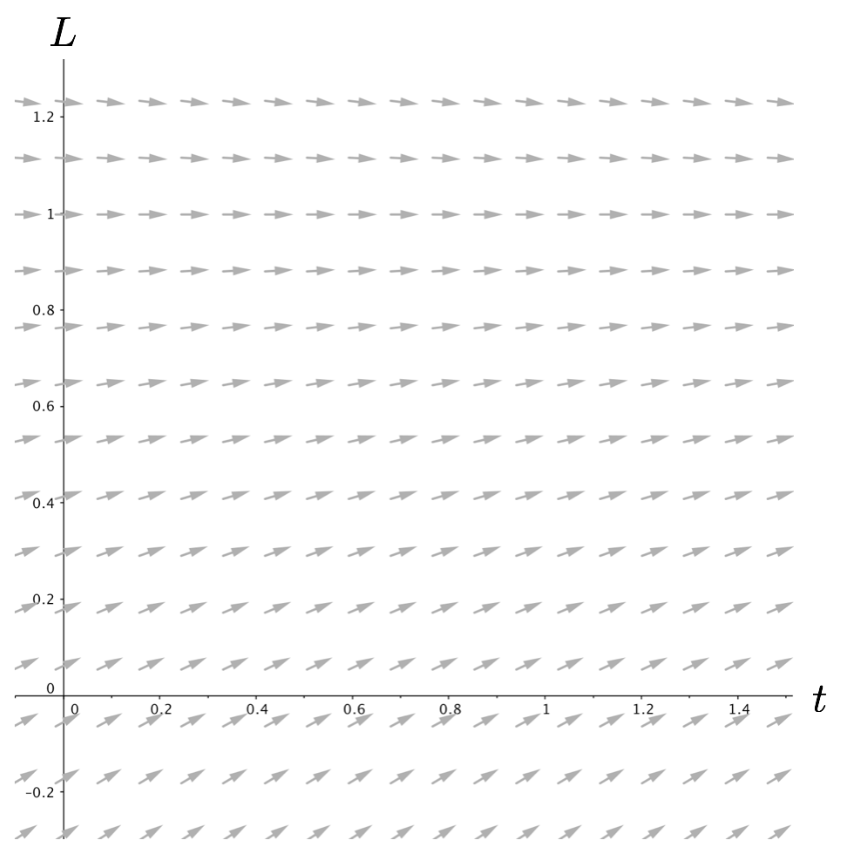
\includegraphics[width=4in]{03/03SlopeField1.png}

\vspace{.5cm}
\textbf{Slope Field} for $\displaystyle\frac{dh}{dt} = -t + 1$

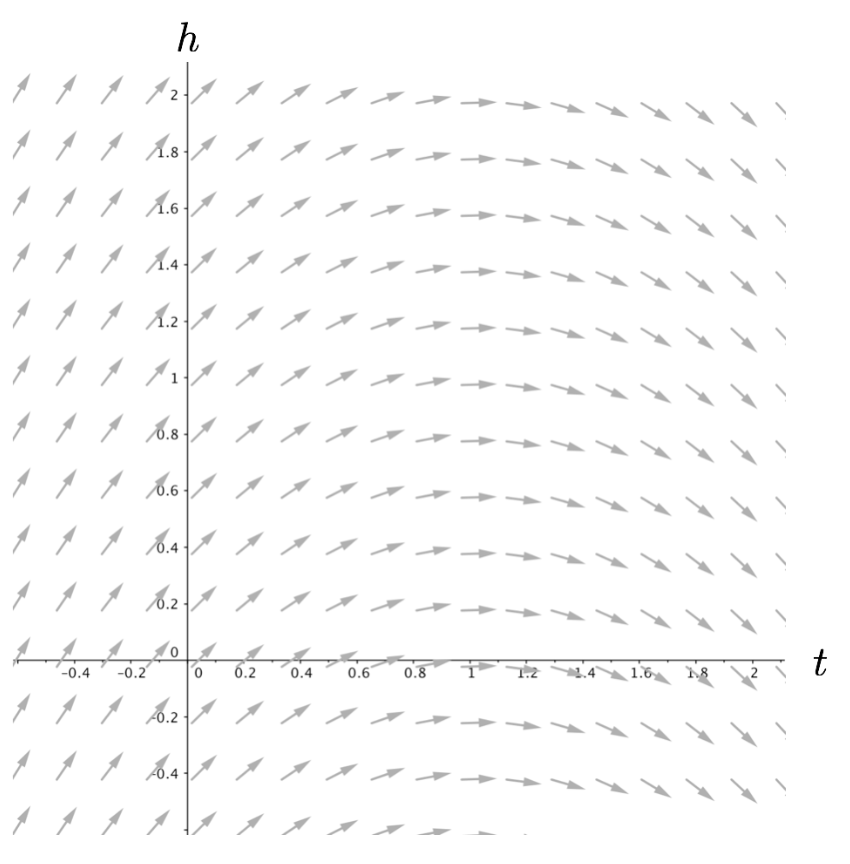
\includegraphics[width=4in]{03/03SlopeField2.png}\\
\end{center}

\clearpage

%%%%%%%%%%%%%%%%%%%%%%%%%%%%%%%%%%%%%%
\pagebegin{Homework Set 3}
\begin{enumerate}

\item When you solve an equation such as $x^2-3=1$ , you get two numbers $x=2$ and $x= -2$.  When you solve a differential equation, what do you get? \label{03HWproblem1}

\item Find the general solution to the following differential equations. \label{03HWproblem2}

\begin{enumerate}
\item $\displaystyle \frac{dy}{dt}=t^4y$
\item $\displaystyle \frac{dy}{dt}=2y+1$
\item $\displaystyle \frac{dy}{dt}=t\sqrt[3]{y}$
\item $\displaystyle \frac{dy}{dt}=\frac{t}{y+1}$
 \item $\displaystyle 2\frac{dy}{dx}=xy(x+1)$
\end{enumerate}
	 
\item	Find the particular solution to the following initial value problems. \label{03HWproblem3}
\begin{enumerate}
\item $\displaystyle \frac{dy}{dt}=\frac{-t}{y}, \qquad y(0)=4$
\item $\displaystyle \frac{dy}{dt}=-\sqrt[3]{y}, \qquad y(0)=27$
\item $\displaystyle \frac{dy}{dx}=\frac{x(y-2)}{x^2+4}, \qquad y(1)=5$
\end{enumerate}
	 
\item	Develop a differential equation where $y(t) = 6$ is a solution function but $y(t) = 8$ is not a solution function. Explain why your differential equation meets both of these criteria. \label{03HWproblem4}

\item Denise has created the following graph to go along with the rate of change equation $\frac{dP}{dt}=0.2P$. \label{03HWproblem5}
\begin{center}
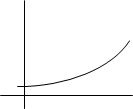
\includegraphics[]{03/03Denise.png}
\end{center}
What is this a graph of? Label the axes and explain your reasoning.

\clearpage

\item Cornelia is working with the differential equation $\displaystyle\frac{dy}{dt}= y - t$.  She has no method like separation of variables to use but still needs to a way to figure out which, if any, of the following functions are solutions to $\displaystyle\frac{dy}{dt}= y - t$. \label{03HWproblem6}
\[
\text{(i) }y(t)= t + 2 \hspace{.75in} \text{(ii) }y(t)= e^t-1 \hspace{.75in} \text{(iii) }y(t) = e^t  + t + 1 \hspace{.75in} \text{(iv) }y(t) = t
\]
  
\begin{enumerate}
\item Read the differential equation $\displaystyle\frac{dy}{dt}= y - t$ with {\em meaning}. Write down exactly how you would read the equation with meaning. Recall {\em reading with meaning} was discussed in Unit 1.
\item	Explain how Cornelia can use a slope field to determine which, if any, of these functions are solutions to the differential equation, $\displaystyle\frac{dy}{dt}= y - t$. 
\item	Use what it means to be a solution to a differential equation to determine which, if any, of these functions are solutions to $\displaystyle\frac{dy}{dt}= y - t$.  Show all work.
\end{enumerate}

\item
\begin{enumerate}
\item Go to the glossary and identify all terms that are relevant to this unit and list those terms here.
\item Are there other vocabulary terms that you think are relevant for this unit that were not included? If yes, list them.
\end{enumerate}

\end{enumerate}


%UNIT 4: LINEAR DIFFERENTIAL EQUATIONS
%%%%%%%%%%%%%%%%%%%%%%%%%%%
%%%% Put the following at the top of each .tex file  %
\pagestyle{fancy}
\renewcommand{\theUnit}{4}
\ifthenelse{\isundefined{\UnitPageNumbers}}{}{\setcounter{page}{1}}
\rhead{Unit \theUnit: Linear Differential Equations}
\lhead{
\includegraphics[width=1.25cm]{IODE-logo.png}}
\rfoot{\mypage}
\lfoot{}
\cfoot{}
\fancypagestyle{firstfooter}{\footskip = 50pt}
\renewcommand{\footrulewidth}{.4pt}
%%%%%%%%%%%%%%%%%%%%%%%%%%%
\vspace*{-20pt} \thispagestyle{firstfooter}
\pagebegin{A Salty Tank}
\begin{enumerate}
\item A very large tank initially contains 15 gallons of saltwater containing 6 pounds of salt. Saltwater containing 1 pound of salt per gallon is pumped into the top of the tank at a rate of 2 gallons per minute, while a well-mixed solution leaves the bottom of the tank at a rate of 1 gallon per minute. \label{04problem1}

\begin{enumerate}
\item Should the rate of change equation for this situation depend just on the amount of salt $S$ in the tank, the time $t$, or both $S$ and $t$? Explain your reasoning. \label{04problem1parta}
\vfill
\item The following is a general rule of thumb for setting up rate of change equations for situations like this where there is an input and an output: \label{04problem1partb}

\[\text{rate of change } = \text{ rate of change in } - \text{ rate of change out}\]

Using the above rule of thumb, figure out a rate of change equation for this situation. \\
{\em Hint}: Think about what the {\em units} of $\frac{dS}{dt}$ need to be, where $S$ is the amount of salt in the tank in pounds.
\vfill

\clearpage

\item	Use the slope field for this differential equation in the GeoGebra applet, \newline\href{https://ggbm.at/PFRcbkbZ}{\underline{https://ggbm.at/PFRcbkbZ}}, to sketch a graph of the solution with initial condition $S(0)=6$. Reproduce this sketch below. Estimate the amount of salt in the tank after 15 minutes. \label{04problem1partc} 
\end{enumerate}
\end{enumerate}

\vspace{-.5in}\hspace{-.1in}
\includegraphics[width=.5in]{04/04SaltyTankQR.png}
\vfill

\clearpage
 
The differential equation you developed for the salty tank is not separable, and therefore using the technique of separation of variables is not appropriate. This differential equation is  called \textbf{first order linear}, which means it has the form 
\[\frac{dy}{dt}+ g(t) \cdot y=r(t),\]
where $g(t)$ and $r(t)$ are both continuous functions. 
\vs
The following technique, which we refer to as the \textbf{reverse product rule}, can be used find the general solution to a first-order linear equation.

\begin{enumerate}[resume]
\item Review the product rule as you remember it from calculus. In general symbolic terms, how do you represent the product rule? How would you describe it in words?
\vfill

Consider the differential equation $\displaystyle\frac{dy}{dt}+2y=3$. Note that this is a first order linear differential equation, where $g(t)$ and $r(t)$ are both continuous functions. The following illustrates a technique for finding the general solution to linear differential equations. The inspiration for the technique comes from a creative use of the product rule and the Fundamental Theorem of Calculus, as well as use of the previous technique of separation of variables.
\begin{center} \renewcommand{\arraystretch}{1.5}
\newcolumntype{V}{>{\arraybackslash} m{.6\linewidth} }
\begin{tabular}{|p{2.5in}|V|}
\hline
Use the product rule to expand $(yu)'$. & \begin{flushright}{\footnotesize Box 0}\end{flushright} \\
{} & {} \\ 
\hline
In the equation $\frac{dy}{dt}+2y=3$, rewrite $\frac{dy}{dt}$ as $y'$.& \begin{flushright}{\footnotesize Box 1}\end{flushright} \\
\hline
Notice that the left-hand side of the equation in Box 1 looks a lot like the expanded product rule but is missing the function $u$.  So multiply both sides by $u$, a function that we will determine shortly.  & \begin{flushright}{\footnotesize Box 2}\end{flushright} \\
\hline
Because, so far, $u$ is an arbitrary function, we can have $u$ satisfy any differential equation that we want. & \begin{flushright}{\footnotesize Box 3}\end{flushright} \\
Use $u' = 2u$ to rewrite the left-hand side of Box 2 to look like Box 0. & {} \\
\hline
%FORCE TABLE TO PAGEBREAK HERE
\end{tabular}\end{center}

\clearpage

\begin{center} \renewcommand{\arraystretch}{1.5}
\newcolumntype{V}{>{\arraybackslash} m{.6\linewidth} }
\begin{tabular}{|p{2.5in}|V|}
\hline
Use separation of variables to solve $u' = 2u$.   & \begin{flushright}{\footnotesize Box 4}\end{flushright} \\
{} & {} \\ 
{} & {} \\ 
\hline
Replace $u$ in the equation from Box 2 with your solution from Box 4. & \begin{flushright}{\footnotesize Box 5}\end{flushright} \\
{} & {} \\ 
\hline
Show that the equation in Box 5 can be rewritten as $\left(ye^{2t}\right)' = 3e^{2t}$ & \begin{flushright}{\footnotesize Box 6}\end{flushright} \\
{\em Hint}: Consider Box 0. & {} \\ 
{} & {} \\ 
\hline
Write integrals with respect to $t$ on both sides.  Apply the Fundamental Theorem of Calculus. & \begin{flushright}{\footnotesize Box 7}\end{flushright} \\
{} & {} \\ 
\hline
Obtain an explicit solution by isolating $y(t)$.& \begin{flushright}{\footnotesize Box 8}\end{flushright} \\
{} & {}\\
\hline
\end{tabular}
\end{center}

\item	Use the previous technique, which we refer to as the \textbf{reverse product rule}, to find the general solution for the Salty Tank differential equation from Problem \ref{04problem1}. \label{04problem3}
\vfill

\clearpage

\item \label{04problem4}
\begin{enumerate}
\item Use the general solution from problem \ref{04problem3} to find the particular solution corresponding to the initial condition $S(0) = 6$ and then use the particular solution to determine the amount of salt in the tank after 15 minutes. That is, compute $S(15)$. Your answer should be close to your estimate from problem \ref{04problem1partc}. Is it? If not, you likely made an algebraic error. \label{04problem4parta}
\vfill
\item What does your solution predict about the amount of salt in the tank in the long run?  How about the concentration? \label{04problem4partb}
\vfill
\item Explain how you can make sense of the predictions from \ref{04problem4partb} by using the differential equation itself. \label{04problem4partc}
\vfill
\end{enumerate}
\newpage

\item Let's call the salty tank from problem \ref{04problem1} Tank A. Consider the following modifications: \label{04problem5}
\begin{itemize}
\item Tank B is the same basic scenario as Tank A, but pure water is being pumped into Tank B instead of saltwater.
\item Tank C is the same  basic scenario as Tank A, but the rates are switched: saltwater enters Tank C at a rate of 1 gallon per minute, and leaves at a rate of 2 gallons per minute.
\item Tank D is the same  basic scenario as Tank A, but Tank D initially contains 6 gallons of pure water.
\end{itemize}
Set up \textbf{but do not solve} initial value problems that correspond to individual Tanks B, C, and D.

\end{enumerate}

\clearpage

%%%%%%%%%%%%%%%%%%%%%%%%%%%%%%%%%%%%%%%%
\pagebegin{Homework Set 4}

\begin{enumerate}
\item Find the general solutions to the following differential equations using separation of variables or the reverse product rule.  Give a reason as to why you used the method you chose over the other. \label{04HWproblem1}

\begin{enumerate}
\item $\displaystyle \frac{dy}{dt}=2y-t$
\item $\displaystyle \frac{dy}{dt}=-\frac{y}{t}+2$
\item $\displaystyle \frac{dy}{dt}=y\sin t$
\item $\displaystyle \frac{dy}{dt}=\cos t$	
\end{enumerate}

\item Solve the following differential equation in two ways: once using separation of variables, and once using the reverse product rule. \label{04HWproblem2} 
\[ \frac{dy}{dt} = 2y+1\, ; \quad y(0)=2\]

\item	For each of the following, determine which method(s) could be used to find the general solution. Do NOT actually find the general solutions, just determine any and all techniques that could be used. \label{04HWproblem3}

\begin{enumerate}
\item $\displaystyle \frac{dy}{dt}=2y-3e^{-t}$
\item $\displaystyle \frac{dy}{dt}=-0.2(75-y)$
\item $\displaystyle \frac{dy}{dt}=y^2+1$
\item $\displaystyle \frac{dy}{dt}=e^t y-\cos t$
\end{enumerate}

\item \label{04HWproblem4}
\begin{enumerate}
\item Create a differential equation (different from all those above) that can only be solved with separation of variables.
\item	Create a differential equation (different from all those above) that can only be solved with the reverse product rule method.
\item	Create a differential equation (different from all those above) that can be solved with either the reverse product rule method or separation of variables.
\end{enumerate}

\item	A tank initially contains 90 lb of salt dissolved in 20 gal of water. Brine containing 2 lb/gal of salt flows into the tank at the rate of 3 gal/min, and the mixture flows out of the tank at the same rate. How much salt does the tank contain 6 minutes later? \label{04HWproblem5}
\vfill

\clearpage

\item \label{04HWproblem6}
\begin{enumerate}
\item Use our technique for solving linear differential equations to verify that the exact solution to $\displaystyle\frac{dy}{dt}=2y-3e^{-t}$ with initial condition $y(0) = 1$ is $y(t) = e^{-t}$.

\item	Compare the long-term behavior of the exact solution and one or more tip to tail Euler's method approximations. Describe and graphically illustrate your results and develop an argument that explains or accounts for these results.

\item The Euler algorithm starts at some value, computes the rate of change at that value, and then assumes that this rate of change is going to be constant over a specified time interval. This process gets you to the next value and the entire process is repeated. In other words, for each time interval this recipe uses the rate of change at the beginning of each interval. One idea to improve this process is instead of using the value of the rate of change at the beginning of each time interval, calculate some sort of average of the rate of change values over the time interval and then use that averaged rate of change just as you would in the Euler recipe. Go to the library and look up in one or more differential textbooks the approximation method called Runge-Kutta. Write down what the algorithm for this method and briefly discuss why this method is better than the Euler method. 

\item	Use EXCEL to compare a Runge-Kutta approximation, an Euler's method approximation, and a graph of the exact solution for the differential equation $\displaystyle\frac{dy}{dt}=2y-3e^{-t}$ with initial condition $y(0) = 1$. Summarize your comparison below and discuss how (and why) the approximations differ from the graph of the exact solution.
\end{enumerate}

\item	Thus far in the course, we have approached analysis of rate of change equations in three different ways -- analytical approaches, numerical approaches, and graphical approaches. In words understandable to a calculus student planning to take differential equations, describe what it means to analytically, numerically, and graphically analyze solutions to a differential equation. Also, develop an explanation that would help this student understand when you might want to use one approach over the other and what advantages and disadvantages each accompanies each approach. \label{04HWproblem7}

\item	Some textbooks refer to the ``reverse product rule'' technique as the method of ``integrating factors.'' Do some research using the internet or textbooks and explain how the integrating factor method relates to the reverse product rule. \label{04HWproblem8}

\item Refer back to problem \ref{04problem5} for the initial value problems you set for for Tanks B, C, and D. Let $B(t)$ be the amount of salt in Tank B, $C(t)$ be the amount of salt in Tank C, and $D(t)$ be the amount of salt in tank D. You should have gotten the following initial value problems:
\[
\frac{dB}{dt}=-\frac{B}{15+t}; \quad B(0)=6
\]
\[
\frac{dC}{dt}=1-\frac{2C}{15-t}; \quad C(0)=6
\]
\[
\frac{dD}{dt}=2-\frac{D}{6+t}; \quad D(0)=0
\]
\begin{enumerate}
\item Solve initial value problems that correspond to individual Tanks B, C, and D.
\item Use a plot to compare four solution curves and discuss how these curves predict/represent outcomes you might expect from the description of each scenario. Refer back to the classwork for the description of the tanks.
\end{enumerate}

\item In this course so far we have discussed various analytic, numerical, and graphical methods and techniques for finding and understanding solutions to differential equations. Below are the methods discussed in this course, up to this point, in the left column. Match the technique to its appropriate category(ies), in the right column. \label{04HWproblem10}

\begin{center}
\begin{tabular}{lll}
\textbf{\underline{Technique}} & \hspace{2in} & \textbf{\underline{Category}} \\
& \hspace{2in} & \\
Euler's Method & \hspace{2in} & Analytic Technique \\
& \hspace{2in} & \\
Reverse Product Rule & \hspace{2in} & Numerical Technique \\
 &\hspace{2in} & \\
Slope Field & \hspace{2in} & Graphical Technique \\
& \hspace{2in} & \\
Separation of Variables & \hspace{2in} &
\end{tabular}
\end{center}

\item
\begin{enumerate}
\item Go to the glossary and identify all terms that are relevant to this unit and list those terms here.
\item Are there other vocabulary terms that you think are relevant for this unit that were not included? If yes, list them.
\end{enumerate}


\end{enumerate}
%UNIT 5: UNIQUENESS OF SOLUTIONS	
%%%%%%%%%%%%%%%%%%%%%%%%%%%
%%%% Put the following at the top of each .tex file  %
\pagestyle{fancy}
\renewcommand{\theUnit}{5}
\ifthenelse{\isundefined{\UnitPageNumbers}}{}{\setcounter{page}{1}}
\rhead{Unit \theUnit: Uniqueness of Solutions}
\lhead{
\includegraphics[width=1.25cm]{IODE-logo.png}}
\rfoot{\mypage}
\lfoot{}
\cfoot{}
\fancypagestyle{firstfooter}{\footskip = 50pt}
\renewcommand{\footrulewidth}{.4pt}
%%%%%%%%%%%%%%%%%%%%%%%%%%%
\vspace*{-20pt} \thispagestyle{firstfooter}
\pagebegin{Proposed Paths of Descent}

A group of scientists at the Federal Aviation Association has come up with the following two different rate of change equations to predict the height of a helicopter as it nears the ground: 
\[ \frac{dh}{dt}=-h \qquad \text{ and } \qquad \frac{dh}{dt}=-h^{\frac{1}{3}}\]
 
For both rate of change equations $h$ is in feet and $t$ is in minutes. The scientists, of course, want their models to predict that a helicopter actually lands - but do either or both of the proposed models predict this? 
\begin{enumerate}
\item Getting familiar with the differential equations: \label{05problem1}

\begin{enumerate}
\item Just by examining the rate of change equations, what can you say about the height of the helicopter as predicted by $\displaystyle\frac{dh}{dt}=-h$  and by $\displaystyle\frac{dh}{dt}=-h^{\frac{1}{3}}$? More specifically, as $h$ approaches zero, what can you say about $\displaystyle\frac{dh}{dt}$ and what does that imply about whether the model predicts that the helicopter lands? \label{05problem1parta}
\vfill

\item Sketch your best guess for a height versus time solution graph for each rate of change equation. \label{05problem1partb}
\end{enumerate}
\vfill

\item	\label{05problem2}
\begin{enumerate}
\item What do each of the proposed rate of change equations say about the solution to the differential equation if the helicopter is already on the ground? Explain and sketch a corresponding graph of height versus time on the same set of axes from part \ref{05problem1partb}. \label{05problem2parta}
\vfill

\item Interpret the initial condition $h(0) = 0$, and explain why $h(t) = 0$ should be a solution to each differential equation under this initial condition. \label{05problem2partb}
\vfill
\end{enumerate}

\clearpage

\item 
\begin{enumerate}
\item Use the Geogebra applet, \href{https://ggbm.at/dJsACfAN}{\underline{https://ggbm.at/dJsACfAN}}, to investigate the slope fields. What do the slope fields suggest about whether the model predicts if the helicopters will land?  How do the slope fields compare with your sketches from part \ref{05problem1partb}? \label{05problem3}

\vspace{-.05in}\hspace{-.5in}
\includegraphics[width=0.5in]{05/05ProposedPathsQR.png}
\vfill
\item On the zoomed in version of the two slope fields from the applet, sketch solution curves for each one. Use $h(0)=0$ and $h(0)=0.2$ as the two initial conditions. \\
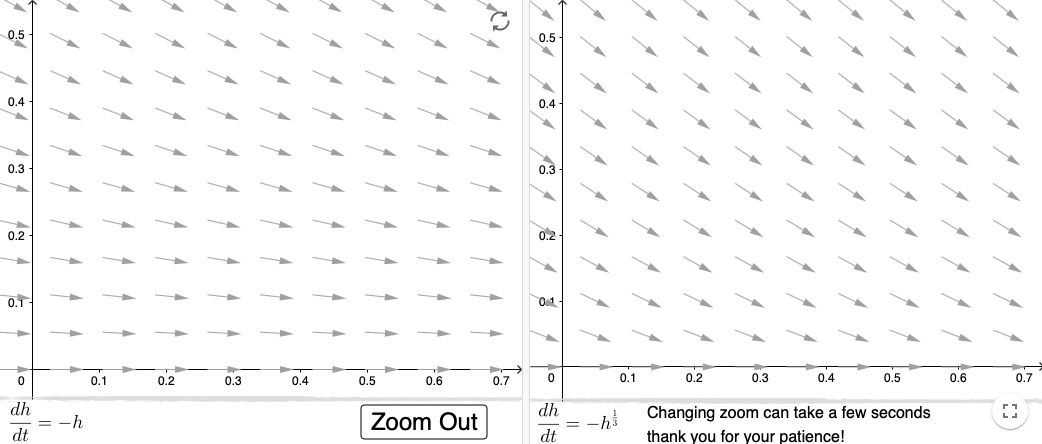
\includegraphics[width=6in]{05/05ZoomedIn.png}
\end{enumerate}
\item Solve the following initial value problems: \label{05problem4}

\begin{enumerate}
\item $\displaystyle\frac{dh}{dt}=-h$

\begin{hnumerate}
\hitem $h(0) = 2$
\hitem $h(0) = 0$ (\textit{Hint}: Use problem \ref{05problem2partb}) \hspace{1in}
\end{hnumerate}
\vfill

\item $\displaystyle\frac{dh}{dt}=-h^{\frac{1}{3}}$
  			                                    
\begin{hnumerate}
\hitem $h(0) = 2$
\hitem $h(0) = 0$ (\textit{Hint}: Use problem \ref{05problem2partb}) \hspace{1in}
\end{hnumerate}
\end{enumerate}
\vfill
\newpage
\item
\begin{enumerate}
\item For each differential equation, interpret the results from problem \ref{05problem4} in terms of whether the model predicts the helicopter will ever touch the ground. If so, at what time? \label{05problem5parta}
\vfill

\item For each differential equation, suppose we know $h\left(\left(\frac{2}{3}\right)^{\frac{3}{2}}\right)=0$. In each case, what is $h(0)$? \label{05problem5partb}
\vfill

\item For each differential equation, interpret the results from problem \ref{05problem4} in terms of whether graphs of (i) and (ii) will ever touch or cross. \label{05problem5partc}
\vfill
\end{enumerate}
\end{enumerate}

\newpage

\pagebegin{The Uniqueness Theorem}

As we saw with the helicopters when $h\left(\frac{2}{3}^{3/2}\right)=0$, it became difficult to predict a value for $h(0)$, because the initial value problem $\displaystyle\frac{dh}{dt}=-h^{\frac{1}{3}};~~$ $h\left(\frac{2}{3}^{3/2}\right)=0$ had multiple solutions. When solutions touch or cross, we lose the predictive power of differential equations. How could we have known that we are safe to use the predictive power of a differential equation without needing the exact solutions? To answer that question, we need the \textbf{Uniqueness Theorem} which gives conditions under which an initial value problem has exactly one solution. \\

In the formal language of differential equations, the term ``unique'' or ``uniqueness'' refers to whether or not two solution functions ever touch or cross each other. Using this terminology, the two solutions you found to $\displaystyle\frac{dh}{dt}=-h$ are unique while the two solutions you found to $\displaystyle\frac{dh}{dt}=-h^{\frac{1}{3}}$ are not unique. Fortunately, one does not have to always analytically solve a differential equation to determine if solutions will or will not be unique. The \textbf{Uniqueness Theorem} sets out conditions for when solutions are unique. \\

\textbf{Theorem.} Let $f(x,y)$ be a real valued function which is continuous on the rectangle 
\[R=\{(x,y):|x-x_0 |\leq a,|y-y_0 |\leq b\}.\]
Assume $f$ has a partial derivative with respect to $y$ and that this partial derivative $\partial f/\partial y$ is also continuous on the rectangle $R$. Then there exists an interval 
\[I = [x_0 - \Delta x, x_0 + \Delta x] \text{ (with $\Delta x \leq a$)}\]
such that the initial value problem 
\[ \frac{dy}{dx}=f(x,y), \qquad y(x_0)=y_0\]
has a unique solution $y(x)$ defined on the interval $I$.

\newpage

\textbf{Informal Theorem.} Suppose we want to know if the graphs of solution functions to a particular rate of change equation $\displaystyle\frac{dy}{dt}=f(t,y)$ are unique. That is, we have decided on a region of the $y$ vs $t$ plane that we care about. For example, suppose we want to know if graphs of solutions to $\displaystyle\frac{dP}{dt}=2P\left(1-\frac{P}{25}\right)$ ever touch or cross the equilibrium solution. Then the region we care about is shown in the dotted rectangle below.

\begin{center}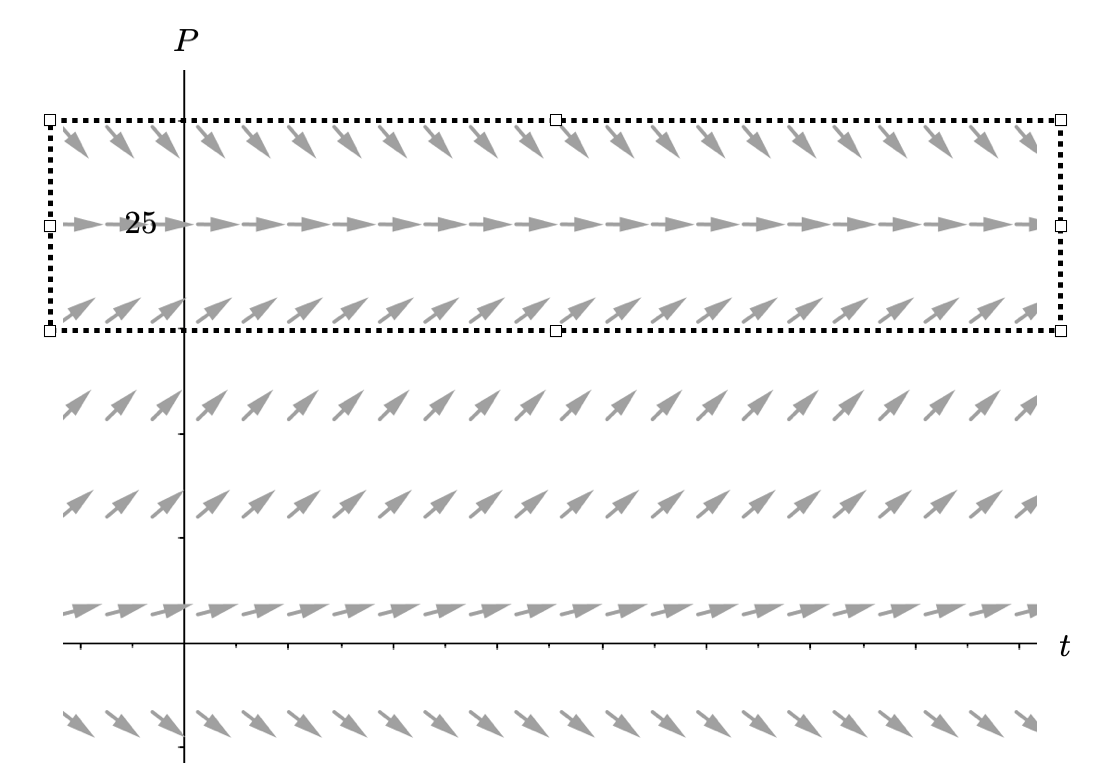
\includegraphics[width=5in]{05/05Dotted.png} \end{center}

Once we have this region established, IF the rate of change of the rate of change, $\displaystyle\frac{\partial}{\partial y}\left(\frac{dy}{dt}\right)$, is continuous in the region we care about. THEN the graphs of the solution functions in this region are guaranteed to be unique. That is, they do not touch or cross each other.

\begin{enumerate}[resume]
\item Discuss how this informal version captures the formal statement of the uniqueness theorem. How would you use this informal version to discuss the predictive power of $\displaystyle\frac{dh}{dt}=-h^{\frac{1}{3}}$? \label{05problem6}
\vfill

\item	If you are given a differential equation and determine that the conditions of the uniqueness theorem are NOT met in a specific range of $y$-values, what can you conclude about the graphs of solution functions within that range of $y$-values? Explain. \label{05problem7}
\vfill
\end{enumerate}

\clearpage

%%%%%%%%%%%%%%%%%%%%%%%%%%%%%%%%%%%%%%
\pagebegin{Homework Set 5}

\begin{enumerate}
\item Suppose two planes start descending at the same time, one is directly above the other and both follow the same differential equation, $\displaystyle\frac{dh}{dt}=-h^{1/3}$. Is there any possibility of a midair collision? Will the initially higher one ever get below the initially lower one? Develop two different arguments to support your conclusion, one based on the uniqueness theorem and one based on the fact this differential equation only depends on $h$ and hence graphs of solutions are related to each in a particular way. \label{05HWproblem1}

\item In light of the \textbf{Uniqueness Theorem}, consider the population model \label{05HWproblem2} 
\[
\frac{dP}{dt}=0.3P\left(1-\frac{P}{12.5}\right).
\]
If $P(0) < 12.5$, will the population ever reach 12.5? Explain.

\item For each differential equation, determine (with reasons) whether or not graphs of solution functions will ever touch any and all equilibrium solution functions (consider both positive and negative values of $t$). \label{05HWproblem3}

\[
\text{(a) } \frac{dL}{dt}=.5(1-L) \hspace{.35in}\text{(b) } \frac{dy}{dt}=0.3y\left(1-\frac{y}{10}\right) \hspace{.35in} \text{(c) } \frac{dy}{dt}=-t+1 \hspace{.35in} \text{(d) } \frac{dy}{dt}=y^{\frac{1}{2}}
\]

\item	Suppose two students are memorizing a list according to the same model  $\displaystyle \frac{dL}{dt}=0.5(1-L)$  where $L$ represents the fraction of the list that is memorized at any time $t$. According to the uniqueness theorem, will the student who starts out knowing none of the list ever catch up to the student who knows one-third of the list? Explain. \label{05HWproblem4}

\item	What values of $p$ result in predictions that the helicopter will land in a finite amount of time for the model $\displaystyle\frac{dh}{dt} = -h^p$? Explain and show all work. \label{05HWproblem5}

\item We could use the equation $\displaystyle\frac{dh}{dt} = h^{\frac{1}{3}}$ to model a helicopter taking off. Suppose we know that $h(0)=0$ and $h(12)=8$. What does $h(12)=8$ mean? When did the helicopter take off? Why did you need to know that the $h(12)=8$ to determine when the helicopter took off? \label{05HWproblem6}

\item Do graphs of solution functions to the rate of change equation $\displaystyle\frac{dy}{dt}=|y|$ ever touch or cross the equilibrium solutions $y(t)=0$?
\begin{enumerate}
\item What does the uniqueness theorem say about this question?
\item Answer this question by solving the rate of change equation. \textsl{Hint: you will need use the piecewise definition of $|y|$ to create two differential equations, one for each ``piece'' and then solve each one separately.} \label{05HWproblem7}
\end{enumerate}

\item \label{05HWproblem8}
\begin{enumerate}
\item Go to the glossary and identify all terms that are relevant to this unit and list those terms here.
\item Are there other vocabulary terms that you think are relevant for this unit that were not included? If yes, list them.
\end{enumerate}

\end{enumerate}






%UNIT 6: AUTONOMOUS DIFFERENTIAL EQUATIONS
%%%%%%%%%%%%%%%%%%%%%%%%%%%
%%%% Put the following at the top of each .tex file  %
\pagestyle{fancy}
\renewcommand{\theUnit}{6}
\ifthenelse{\isundefined{\UnitPageNumbers}}{}{\setcounter{page}{1}}
\rhead{Unit \theUnit: Autonomous Differential Equations}
\lhead{
\includegraphics[width=1.25cm]{IODE-logo.png}}
\rfoot{\mypage}
\lfoot{}
\cfoot{}
\fancypagestyle{firstfooter}{\footskip = 50pt}
\renewcommand{\footrulewidth}{.4pt}
%%%%%%%%%%%%%%%%%%%%%%%%%%%
\vspace*{-20pt} \thispagestyle{firstfooter}
\pagebegin{Analyzing Autonomous DEs: Spotted Owls}

A group of biologists are making predictions about the spotted owl population in a forest in the Pacific Northwest.  The autonomous differential equation the scientist use to model the spotted owl population is $\displaystyle \frac{dP}{dt}=\frac{P}{2}\left(1-\frac{P}{5}\right)\left(\frac{P}{8}-1\right)$, where $P$ is in hundreds of owls and $t$ is in years. The problem is that the current number of owls is only approximately known.  
\begin{enumerate}
\item Suppose the scientists estimate that currently $P$ is about 5 (i.e. there are currently about 500 owls in the forest).  Since 5 is only an estimate, they make long-term predictions of the owl population for the initial conditions $P = 4.9$, $P = 5.0$, and $P = 5.1$. \textit{Without using a graphing calculator or other software}, determine the long-term predictions for these initial conditions based on the differential equation. Are they similar or different?  That is, will slightly different initial conditions yield only slightly different long-term predictions, or will they be radically different? Carry out a similar analysis if the current number of owls is somewhere around 8.\label{06problem1}
\vspace{4in}

\item Give a one dimensional representation, \textit{without words}, that would describe all solutions to the differential equation. \label{06problem2}

\clearpage
\item A \textbf{phase line} is the standard one-dimensional diagram that depicts the qualitative behavior of solutions to an autonomous differential equation. Label (and modify, if necessary) the dots and add arrows to the figure below to represent \textbf{all} solutions to the differential equation in Problem \ref{06problem1}. \label{06problem3} \\
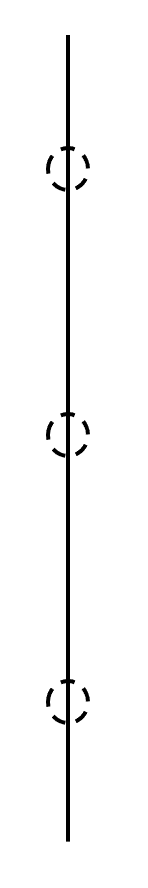
\includegraphics[width=.75in]{06/06PhaseLine.png}

\item For the differential equation in problems \ref{06problem1}-\ref{06problem3} there are three equilibrium solutions. Recall that equilibrium solutions are constant functions that satisfy the differential equation. How do the other solution functions near each equilibrium solution behave in the long term? If you were to label each of these equilibrium solutions based on the way in which nearby solutions behave, what terms would you use and why? \label{06problem4} 

\end{enumerate}

\clearpage

\pagebegin{Phase Lines}

\begin{enumerate}[resume]
\item Dominique is working with the rate of change equation $\frac{dP}{dt}=0.2P$  and thinks about solutions in terms of whether they are increasing, decreasing, or remaining constant. She illustrates her thinking with the phase line shown below. 
\begin{center}
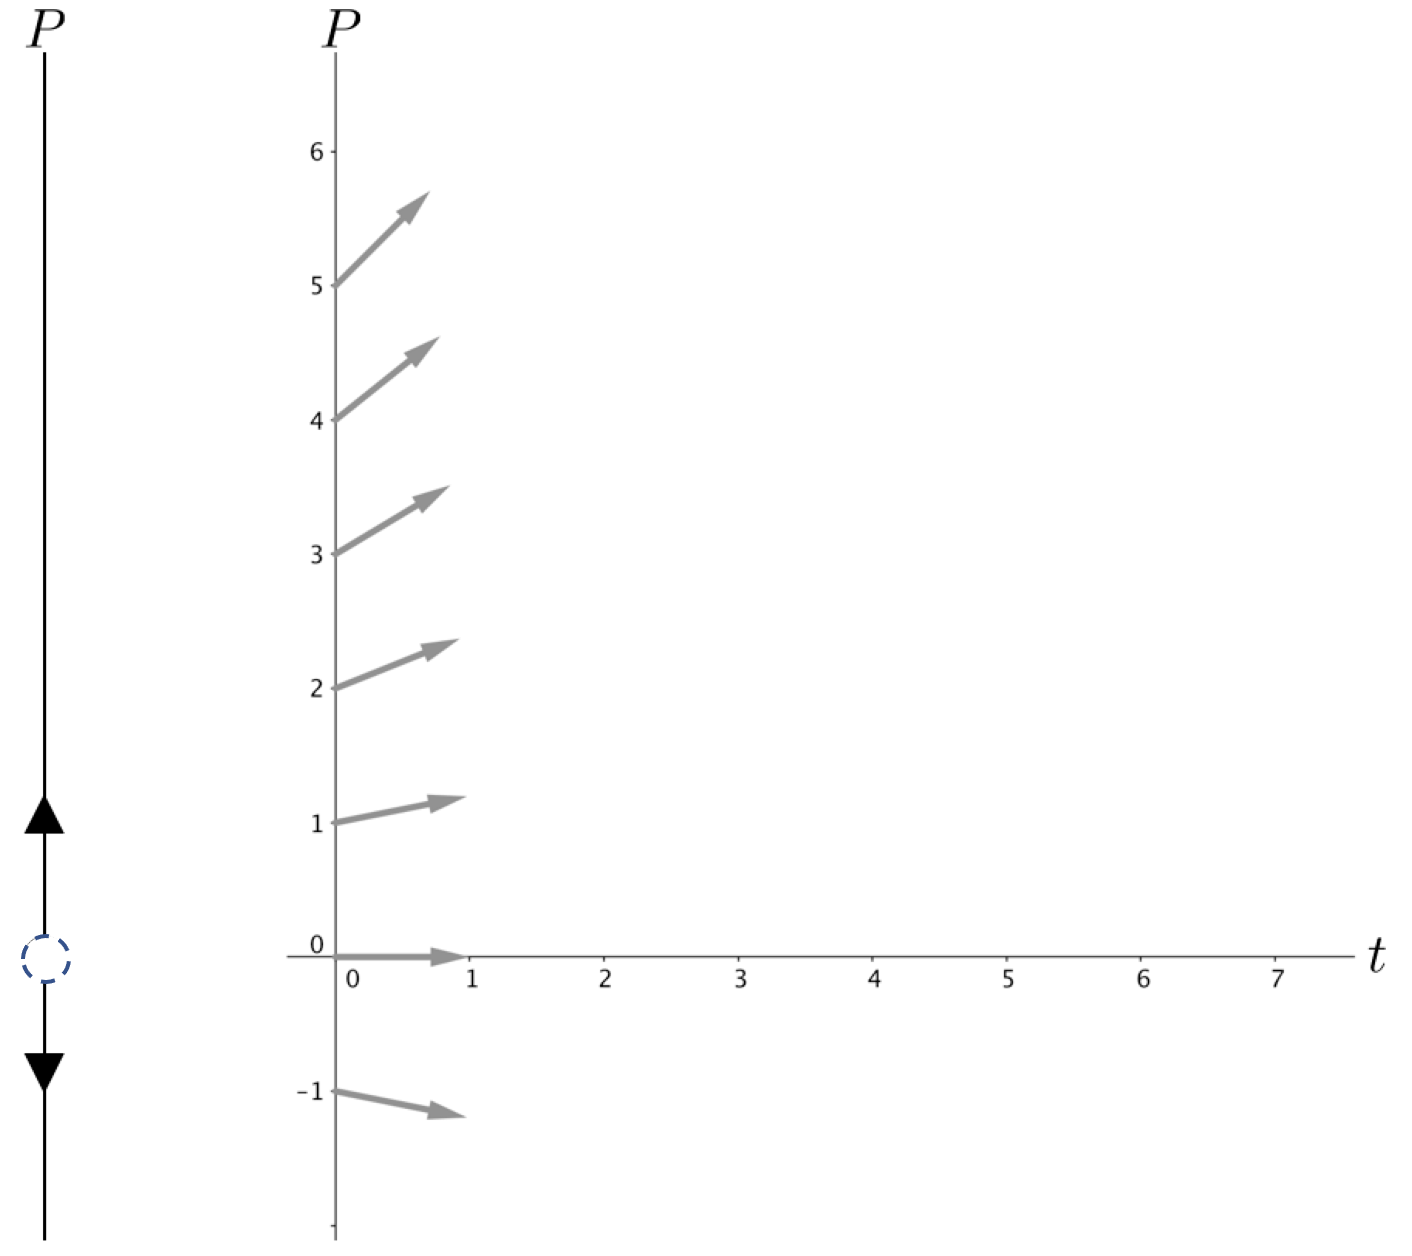
\includegraphics[width=6in]{06/06PhaseLineAndSomeVectors.png} \\
\end{center}
\clearpage
\begin{enumerate}
\item	Place your fingertip or other small item on the phase line at $P = 0$ and another fingertip or small item at $P = 0$ on the $P$ vs $t$ axes and imagine time moving forward. Explain, with reasons, what happens to your fingertips. \label{06problem5parta} \vfill

\item	Place your fingertip or other small item on the phase line at $P = 1$ and another fingertip or small item at $P = 1$ on the $P$ vs $t$ axes at (0,1) and imagine time moving forward. Explain, with reasons, what happens to your fingertips. \label{06problem5partb}   \vfill

\item	Place two fingertips or two small items on the phase line, one at $P = 1$ and the other at $P = 3$. What happens to your fingertips as time moves forward? How do your ideas relate to the corresponding $P$ versus $t$ graphs? \label{06problem5partc}  \vfill

\item	Explain how a person could think about the phase line as a one-dimensional projection of all of the two-dimensional $P(t)$ graphs of solutions. \label{06problem5partd} \vfill

\end{enumerate}
\end{enumerate}
\clearpage

%%%%%%%%%%%%%%%%%%%%%%%%%%%%%%%%%%%%%%%%%%%%%%%%%%%%%%%%%%%%%%%%%%%%%%%%%%%%%%%%%%%%%%%%%%
\pagebegin{Homework Set 6}

\begin{enumerate}
\item For an autonomous differential equations, it is possible to view all of the solution function graphs in terms of ``prototypical'' graphs. A prototypical solution graph represents an infinite number of other solution graphs. For example, in part (i) below one can view the entire family of functions that solve the differential equation in terms of two different prototypical solution graphs separated by an equilibrium solution: one prototypical solution graph is above the $t$-axis and one is below the $t$-axis. Each is prototypical because it can stand for all other solution graphs (in its respective region) through horizontal translation. Recall the ``Making Connections'' section of Unit 3. \label{06HWproblem1}
\begin{hnumerate}
\hitem    $\displaystyle\frac{dy}{dt}=-y$    \hitem $\displaystyle\frac{dy}{dt}=2y\left(1-\frac{y}{2}\right)$        \hitem $\displaystyle\frac{dy}{dt}=2y\left(1-\frac{y}{2}\right)+3$        \hitem   $\displaystyle\frac{dy}{dt}=y^2$ \end{hnumerate}
\begin{enumerate}
\item For each differential equation above, draw a phase line and representative graphs of solutions. \label{06HWproblem1parta}
\item For each differential equation above, explain how your response to number \ref{06HWproblem1parta} can be interpreted in terms of prototypical solutions separated by equilibrium solutions. \label{06HWproblem1partb} 
\end{enumerate}

\item For each of the following slope fields, create a differential equation whose slope field would be similar to the one given. Give reasons for why you created the differential equation as you did. You may create whatever scale on the axes that you want. \label{06HWproblem2} \\
\begin{enumerate*}
\item 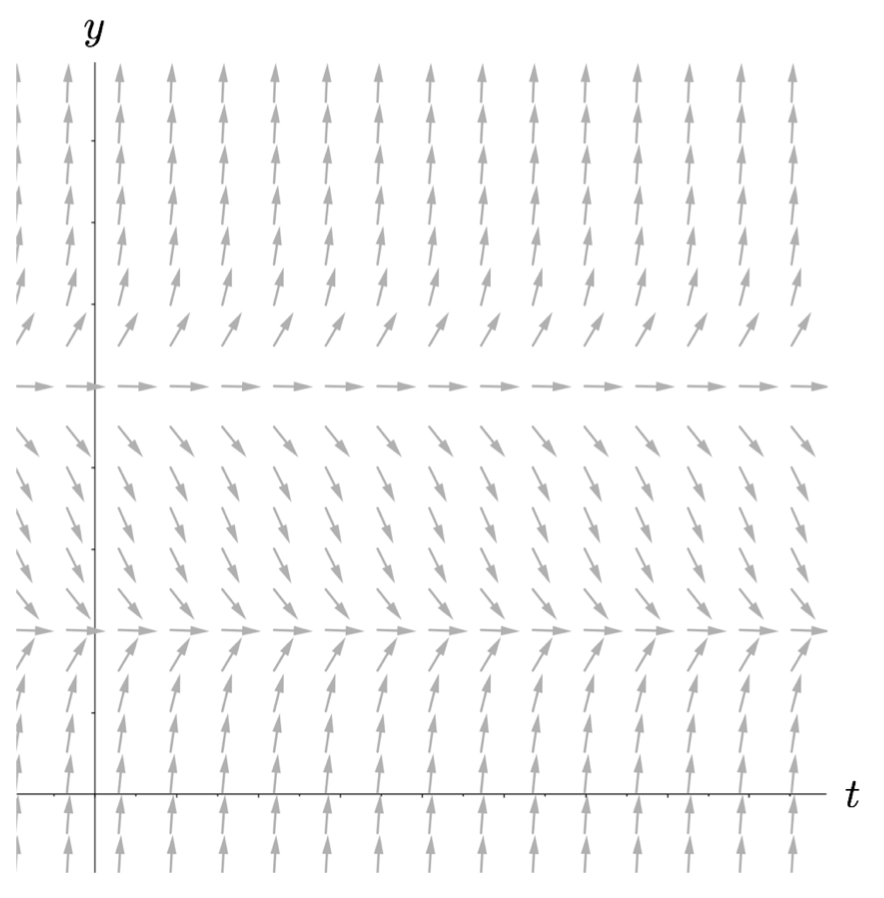
\includegraphics[width=3in]{06/06HWSlopeFieldA.png}
\item 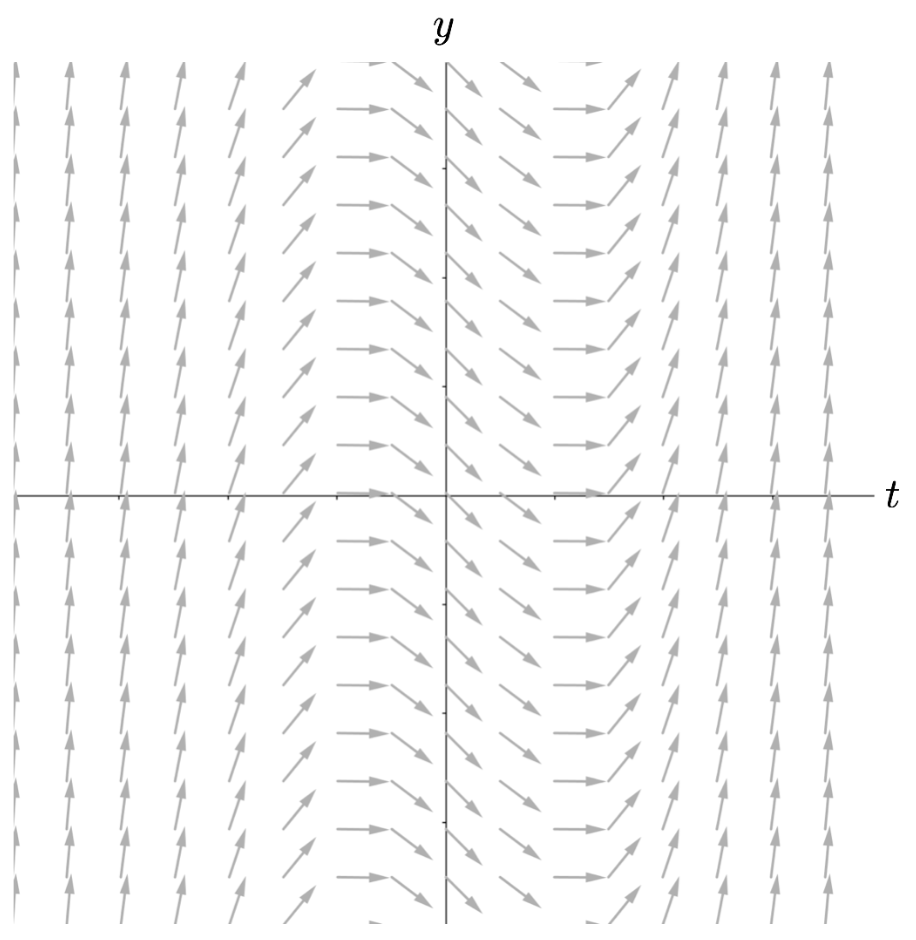
\includegraphics[width=3in]{06/06HWSlopeFieldB.png}
\item 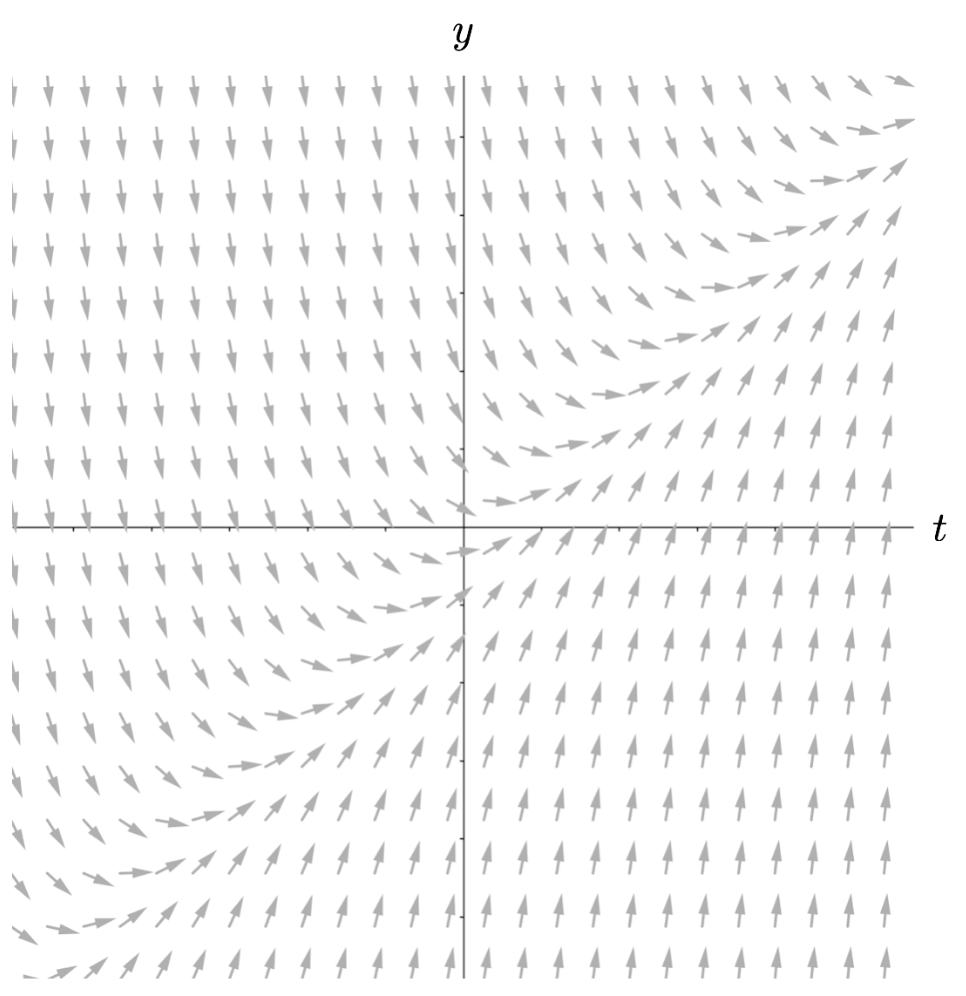
\includegraphics[width=3in]{06/06HWSlopeFieldC.png}
\item 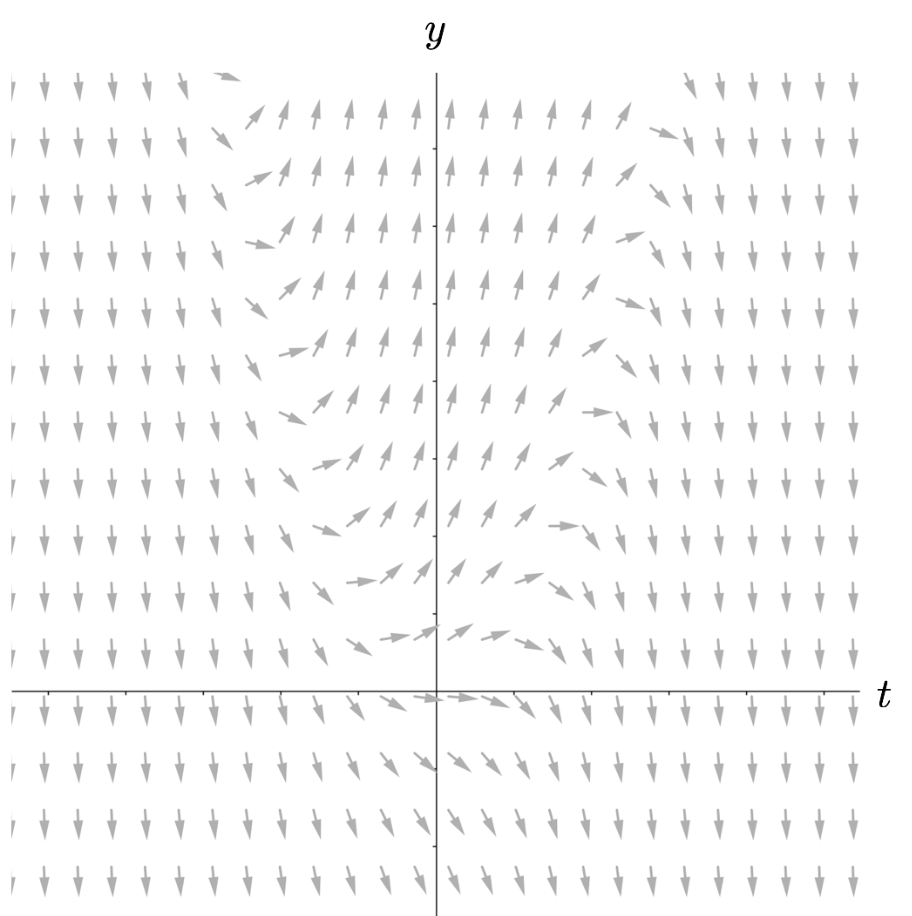
\includegraphics[width=3in]{06/06HWSlopeFieldD.png}
\end{enumerate*}

\item For each part below, create a continuous, autonomous differential equation that has the stated properties (if possible). Explain how you created each differential equation and include all graphs or diagrams you used and how you used them. If it is not possible to come up with a differential equation with the stated properties, provide a justification for why it cannot be done. \label{06HWproblem3}

\begin{enumerate}
\item Exactly three constant solution functions, two repellers and one attractor.
\item	Exactly two constant solution functions, one a repeller and one a node.
\item	Exactly two constant solution functions, both attractors.
\end{enumerate}

\item For each part below, create an autonomous differential equation that satisfies the stated criteria \label{06HWproblem4}
\begin{enumerate}
\item	$y(t)=0$ and $y(t) = -4$ are the only constant solution functions
\item $y(t)=e^{-t+1}$ is a solution
\item $y(t)=e^{2t-5}$	is a solution
\item $y(t)=10e^{0.3t}$ is a solution
\item $y(t)=1-e^{-t}$ and $y(t)=1+e^{-t}$ are solutions
\end{enumerate}

\item For a phase line to be a meaningful tool, explain why it is essential for the differential equation to be autonomous. \label{06HWproblem5}

\item In class you and your classmates continue to develop creative and effective ways of thinking about particular ideas or problems. Discuss at least one idea or way of thinking about a particular problem that has been discussed in class (either in whole class discussion or in small group) that was particularly helpful for enlarging your own thinking and/or that you disagreed with and had a different way of thinking about the idea or problem. \label{06HWproblem6}

\item \label{06HWproblem7}
\begin{enumerate}
\item Go to the glossary and identify all terms that are relevant to this unit and list those terms here.
\item Are there other vocabulary terms that you think are relevant for this unit that were not included? If yes, list them.
\end{enumerate}

\end{enumerate}
%UNIT 7: MODELING WITH AUTONOMOUS DIFFERENTIAL EQUATIONS
%%%%%%%%%%%%%%%%%%%%%%%%%%%
%%%% Put the following at the top of each .tex file  %
\pagestyle{fancy}
\renewcommand{\theUnit}{7}
\ifthenelse{\isundefined{\UnitPageNumbers}}{}{\setcounter{page}{1}}
\rhead{Unit \theUnit: Modeling with Autonomous Differential Equations}
\lhead{
\includegraphics[width=1.25cm]{IODE-logo.png}}
\rfoot{\mypage}
\lfoot{}
\cfoot{}
\fancypagestyle{firstfooter}{\footskip = 50pt}
\renewcommand{\footrulewidth}{.4pt}
%%%%%%%%%%%%%%%%%%%%%%%%%%%
\vspace*{-20pt} \thispagestyle{firstfooter}
\pagebegin{Cooling Coffee}

\includegraphics[]{07/07CoffeeCup.png}
A group of students want to develop a rate of change equation to describe the cooling rate for hot coffee in order that they can make predictions about other cups of cooling coffee. Their idea is to use a temperature probe to collect data on the temperature of the coffee as it changes over time and then to use this data to develop a rate of change equation. \\

The data they collected is shown in the table below. The temperature C (in degrees Fahrenheit) was recorded every 2 minutes over a 14 minute period. \\

\begin{tabular}{|c|c|}
\hline
Time (min) & Temp. (\degree F)\\\hline
0 & 160.3\\\hline
2 & 120.4\\\hline
4 & 98.1\\\hline
6 & 84.8\\\hline
8 & 78.5\\\hline
10 & 74.4\\\hline
12 & 72.1\\\hline
14 & 71.5\\\hline
\end{tabular}
\begin{enumerate}
\item Figure out a way to use this data to create a third column whose values approximate  $\displaystyle\frac{dC}{dt}$, where $C$ is the temperature of the coffee.\label{07problem1} \vfill

\item	Do you expect $\displaystyle\frac{dC}{dt}$ to depend on just the temperature $C$, on just the time $t$, or both the temperature $C$ and the time $t$? \label{07problem2} \vfill

\item Sketch below your best guess for the graph of $\displaystyle\frac{dC}{dt}$. \label{07problem3}
\begin{center}
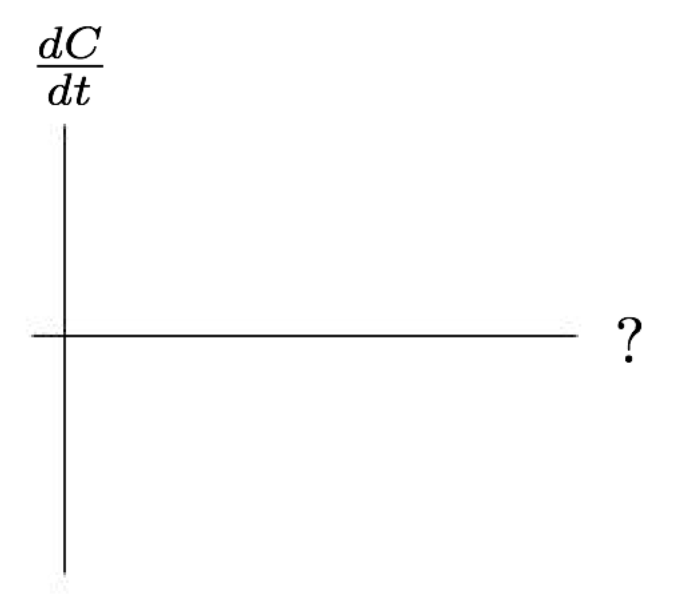
\includegraphics[width=3in]{07/07dCdt.png}
\end{center}

\clearpage
\item
\begin{enumerate} \label{07problem4} 
\item Input the data from your extended table in question \ref{07problem1} into the GeoGebra applet \\\href{https://ggbm.at/uj2gbz3V}{\underline{https://ggbm.at/uj2gbz3V}} to plot points for $\displaystyle\frac{dC}{dt}$ vs. $C$. Does this plot confirm or reject your sketch from question \ref{07problem3}? 
\vspace{1.5in}
\item Toggle on the curve fitting tool and find an equation that fits your data.
\end{enumerate} 

\vspace{-2in}\hspace{-0.5in}
\includegraphics[width=0.5in]{07/07CoolingCoffeeQR.png}
\vfill

\clearpage

\item One group of students figured out that a reasonable rate of change equation to be \[ \frac{dC}{dt}=-0.4C+28\]   which they rewrote as  \[\displaystyle \frac{dC}{dt}=-0.4\left(C-70\right).\] Interpret the meaning of the number $70$ in this equation. Does this rate of change equation also make sense for predicting the future temperature of a glass of ice tea? Why or why not? \label{07problem5}
\vfill
\item	According to the rate of change equation from questions \ref{07problem4} and \ref{07problem5}, is it possible for a graph of the \bf exact \rm solution to look like the one below? Why or why not? Give more than one reason for your answer. \label{07problem6}
\begin{center}
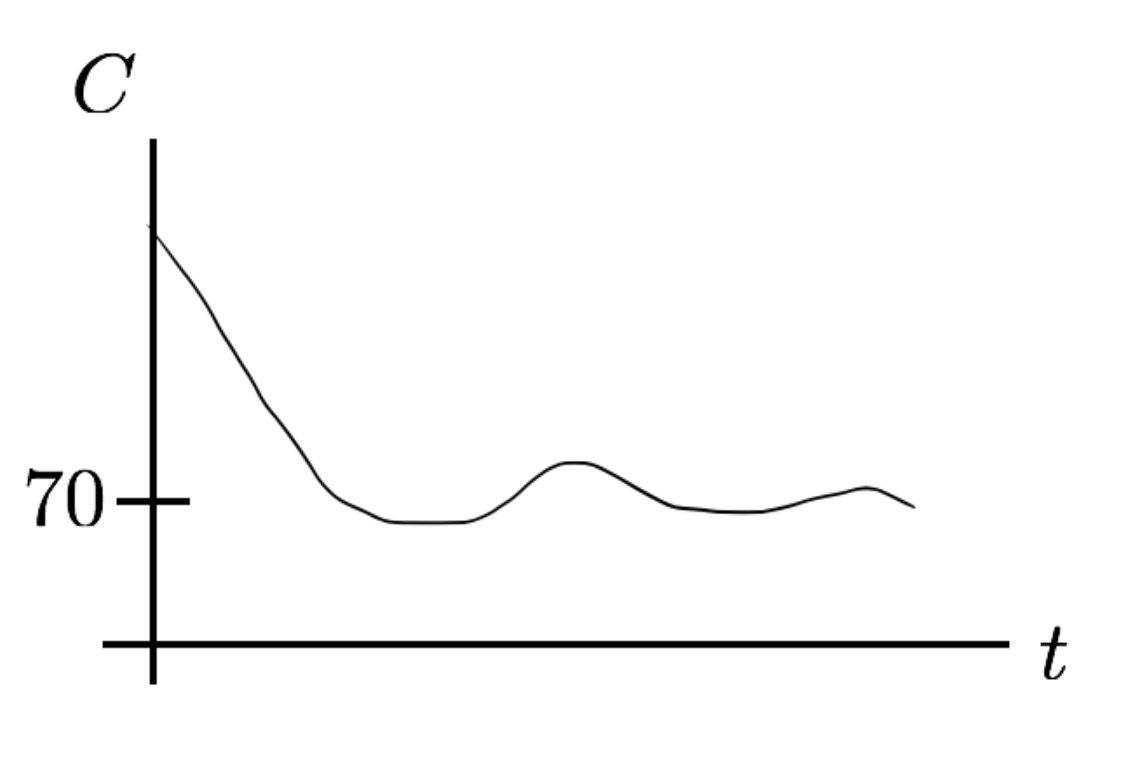
\includegraphics[width=3in]{07/07CoffeeEquilibrium.png}
\end{center}
\vfill

\end{enumerate}
\clearpage

%%%%%%%%%%%%%%%%%%%%%%%%%%%
\pagebegin{Population Growth - Limited Resources}
A group of biologists want to study the population growth of certain bacteria in a laboratory. The scientists realized that the culture for the bacteria does not provide unlimited resources. Hence, the rate of change equation $\displaystyle\frac{dP}{dt}=kP$ is not appropriate. They conducted experiments to determine how the rate of change of population depends on just the population. The data they collected is shown in the table below (numbers are properly scaled). At various population levels, the scientists measured the population after one day. \\

\begin{tabular}{|c|c|}
\hline
\parbox{1in}{Beginning\\ Population} & \parbox{1.5in}{Population after\\ one day}\\ \hline 
2 & 2.34\\ \hline 
4 & 4.54\\ \hline 
6 & 6.62\\ \hline 
8 & 8.58\\ \hline 
10 & 10.40\\ \hline 
12 & 12.10\\ \hline 
14 & 13.66\\ \hline 
16 & 15.10\\ \hline 
18 & 16.42\\ \hline 
20 & 17.60\\ \hline 

\end{tabular}

\begin{enumerate}[resume]
\item	Create a third column whose values approximate $\frac{dP}{dt}$. Explain why the method you used to create this column makes sense.\label{07problem7}\vfill



\item	In this course we will call a graph of $\frac{dP}{dt}$ vs. $P$, when $\frac{dP}{dt}$ is an autonomous differential equation, an \textbf{Autonomous Derivative Graph}. Create an \textbf{autonomous derivative graph} and figure out a way to analyze this graph to determine the long term behavior for each of the beginning populations given in the table above.\label{07problem8}
\vfill
\end{enumerate}

\clearpage

%%%%%%%%%%%%%%%%%%%%%%%%%%%%%%%
\pagebegin{Analyzing Graphs of Autonomous Differential Equations}

\begin{enumerate}[resume]
\item A group of biologists is studying a particular bug population in a rainforest. They gathered data about these bugs for different population values, $N$, at different times, $t$. The scientists reasoned that the rate of change depended only on the population and not on time. They approximated the derivatives $\frac{dN}{dt}$ (as was done with the cooling coffee from before) and plotted the autonomous derivative graph, as seen below: \label{07problem9}
\begin{center}
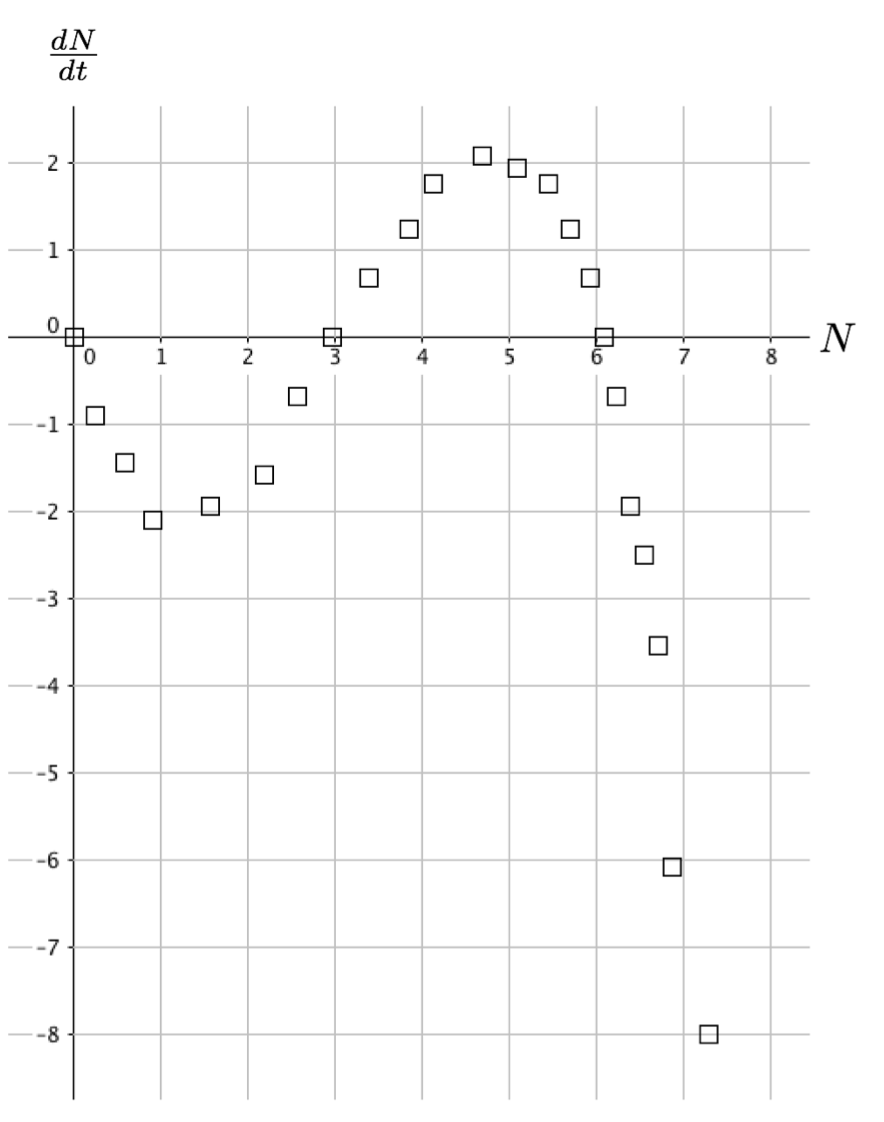
\includegraphics[width=3.5in]{07/07Bugs1.png}
\end{center}
For each part below, use the autonomous derivative graph to predict what the ultimate fate of the population will be. Describe (in words) the long-term behavior of each solution corresponding to the given initial condition. In addition, illustrate your conclusions with a suitable graph or graphs and classify all equilibrium solutions as either an attractor, repeller, or node.

\begin{enumerate}
\item	$N(0) = 2$ 
\item	$N(0) = 3$
\item	$N(0) = 4$
\item	$N(0) = 4.5$
\item	$N(0) = 6$
\item	$N(0) = 8$
\end{enumerate}

\clearpage
\item	Below is an autonomous derivative graph. Figure out the long-term behavior of \underline{every} possible solution function and illustrate your conclusions with a suitable graph or graphs. \label{07problem10}
\begin{center}
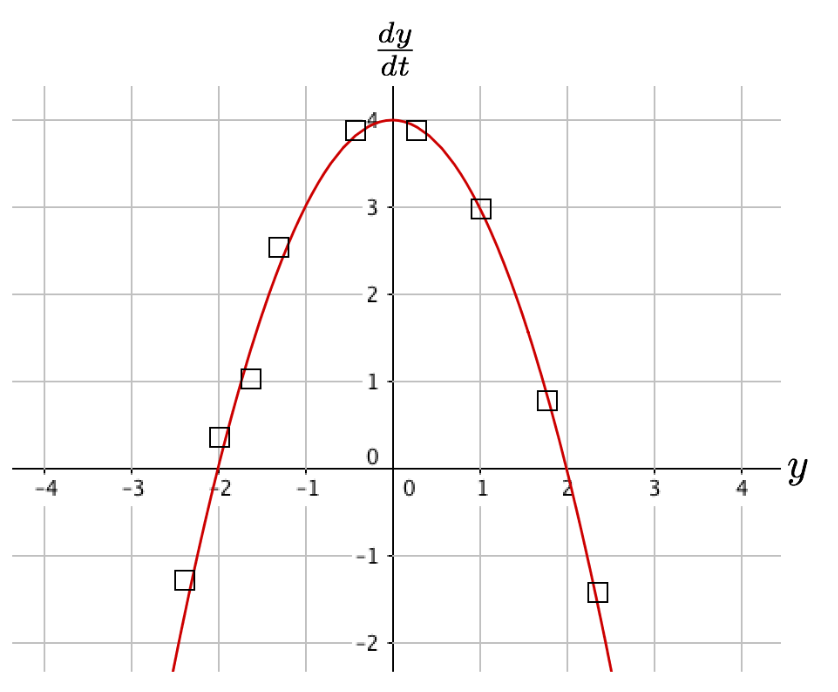
\includegraphics[width=3.5in]{07/07Bugs2.png}
\end{center}

\end{enumerate}

\clearpage
%%%%%%%%%%%%%%%%%%%%%%%%%%%%%%%%%%%%%%%%
\pagebegin{Homework Set 7}

\begin{enumerate}
\item  For this problem, use the coffee cooling rate of change equation  \[\displaystyle \frac{dC}{dt}=-0.4C+28.\] \label{07HWproblem1}
\begin{enumerate}
\item	Is there ever a time when two cups of coffee, one at initially 160\degree F and one at 180\degree F, are the exact same temperature? Answer this question according to the uniqueness theorem. Comment on whether your answer matches what you expect to happen in real life? 
\item	How long will it take a cup of hot coffee that is initially 180\degree F to cool down to 100\degree F? Use the reverse product rule to figure this out and then check the reasonableness of your answer with Euler's method.

\end{enumerate}
\item	For each part below you are provided with an autonomous derivative graph. Figure out the long-term behavior of every possible solution function. Illustrate your conclusions with representative $y(t)$ solution graphs and summarize your findings about the long-term behavior of different solutions in paragraph form. \label{07HWproblem2} \\
\begin{enumerate*}
\item 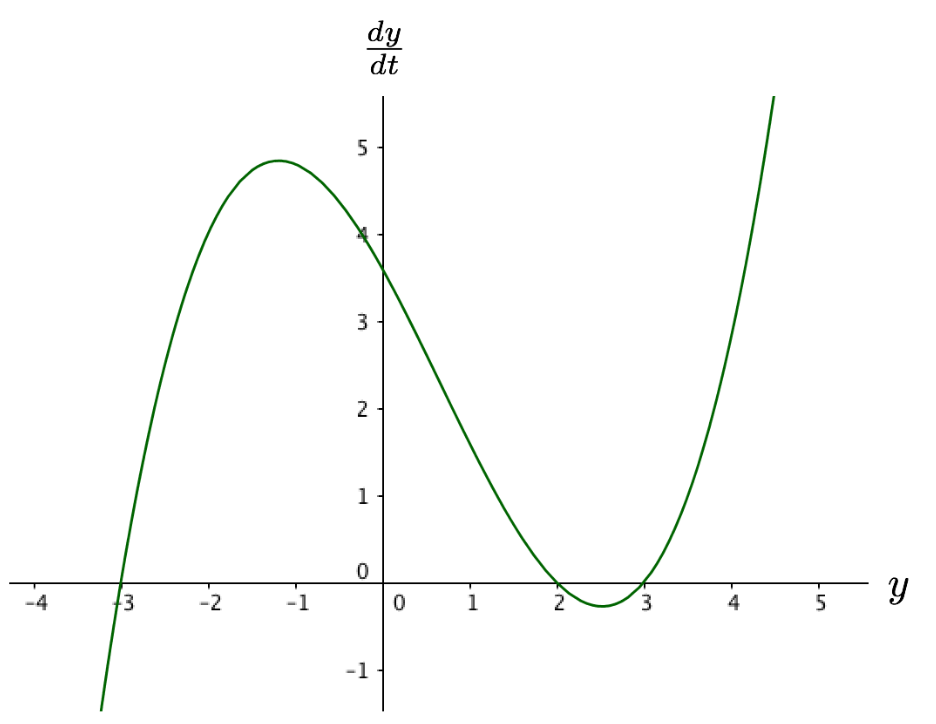
\includegraphics[width=3in]{07/07HWgraph1.png} \label{07HWproblem2parta}
\item 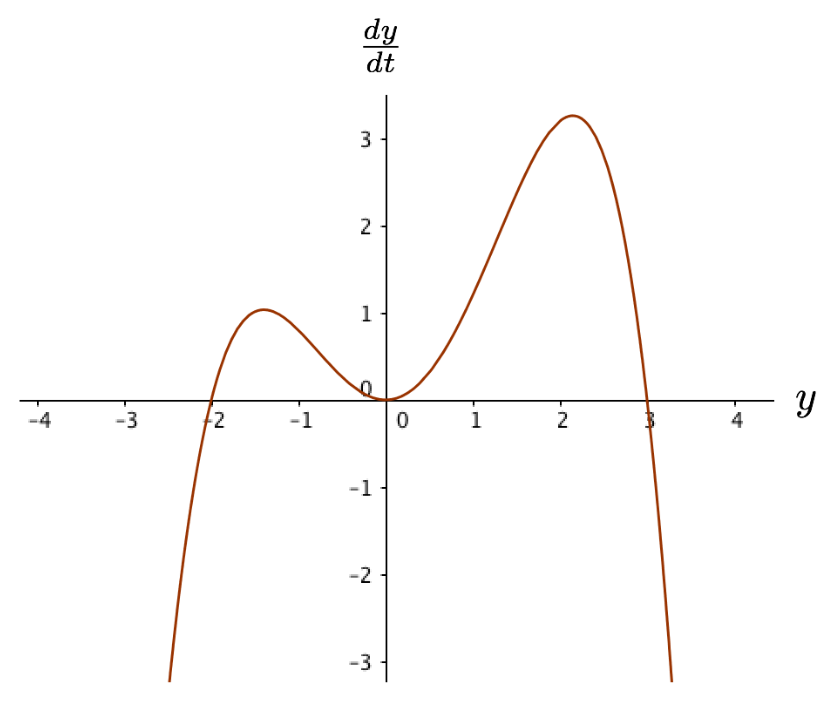
\includegraphics[width=3in]{07/07HWgraph2.png} \label{07HWproblem2partb}
\end{enumerate*}
\item	For each part in problem \ref{07HWproblem2}, create a phase line and classify each equilibrium solution as either an attractor, repeller, or node. \label{07HWproblem3}

\item	For problem \ref{07HWproblem2partb}, use the uniqueness theorem to determine if any of the non-constant solution functions ever reach the equilibrium solution of $y(t)=0$ in a finite amount of time. \label{07HWproblem4}

\item	Given an autonomous differential equation $\frac{dy}{dt}=f(y)$ , give a general strategy for how to use an autonomous derivative graph to determine the long term behavior of solution functions. \label{07HWproblem5}

\clearpage

\item	Suppose you wish to predict future values of some quantity, $y$, using an autonomous differential equation (that is, $dy/dt$ depends explicitly only on $y$). Experiments have been performed that give the following information: \label{07HWproblem6}
\begin{itemize}
\item	The only equilibrium solutions are $y(t)=0$, $y(t)=15$, and $y(t)=60$
\item	If the value of $y$ is 100, the quantity decreases
\item	If the value of $y$ is 30, the quantity increases
\item	If the value of $y$ is negative, the quantity increases
\end{itemize}

\begin{enumerate}
\item	How many different phase lines match the above? Sketch all possible phase lines. \label{07HWproblem6parta}
\item	Provide a rough sketch of an autonomous derivative graph for each of your phase lines in part \ref{07HWproblem6parta}. \label{07HWproblem6partb}
\item	For each of your different sketches in part \ref{07HWproblem6partb}, develop a differential equation that fits the basic features. \label{07HWproblem6partc}
\end{enumerate}
\item  In what ways is the letter $y$ in the differential equation $\frac{dy}{dt} = .3y$ both a variable and a function? In what ways is $\frac{dy}{dt}$ a function? \label{07HWproblem7}
\item Newton's law of cooling is an empirical law that states that an object immersed in a constant, ambient temperature will have its temperature change at a rate proportional to the difference between the its temperature and the ambient temperature. Explain how the cooling coffee problem reflects Newton's law of cooling. \label{07HWproblem8}
\item A body was found in a temperature controlled environment (i.e., you know the room temperature) and is subject to Newton's law of cooling. Explain why you only need the room temperature and the measurement of the body's temperature at two different times to give an estimate of the time of death. \label{07HWproblem9}
\item Are the following true or false statements? Explain your reasoning. \label{07HWproblem10}
\begin{enumerate}
\item If the autonomous derivative graph has a vertical tangent line at some point, then according to the uniqueness theorem, solutions to the differential equation are guaranteed to touch or cross at that point.  
\item If the autonomous derivative graph is a polynomial, then according to the uniqueness theorem, solutions to the differential equation are everywhere unique.
\end{enumerate}
\item \label{07HWproblem11}
\begin{enumerate}
\item Go to the glossary and identify all terms that are relevant to this unit and list those terms here.
\item Are there other vocabulary terms that you think are relevant for this unit that were not included? If yes, list them.
\end{enumerate}

\end{enumerate}




%UNIT 8: THE EFFECT OF VARYING A PARAMETER IN AUTONOMOUS DIFFERENTIAL EQUATIONS
%%%%%%%%%%%%%%%%%%%%%%%%%%%
%%%% Put the following at the top of each .tex file  %
\pagestyle{fancy}
\renewcommand{\theUnit}{8}
\ifthenelse{\isundefined{\UnitPageNumbers}}{}{\setcounter{page}{1}}
\rhead{Unit \theUnit: The Effect of Varying a Parameter in Autonomous Differential Equations}
\lhead{\includegraphics[width=1.25cm]{IODE-logo.png}}
\rfoot{\mypage}
\lfoot{}
\cfoot{}
\fancypagestyle{firstfooter}{\footskip = 50pt}
\renewcommand{\footrulewidth}{.4pt}
%%%%%%%%%%%%%%%%%%%%%%%%%%%
\vspace*{-20pt} \thispagestyle{firstfooter}
\pagebegin{Fish Harvesting}

A mathematician at a fish hatchery has been using the differential equation $\displaystyle\frac{dP}{dt}=2P\left(1-\frac{P}{25}\right)$ as a model for predicting the number of fish that a hatchery can expect to find in their pond.

\begin{enumerate}
\item Use an autonomous derivative graph, a phase line, and a slope field to analyze what this differential equation predicts for future fish populations for a range of initial conditions. Present all three of these representations and describe in a few sentences how to interpret them. \label{08problem1}
\clearpage

\item	Recently, the hatchery was bought out by fish.net and the new owners are planning to allow the public to catch fish at the hatchery (for a fee of course). This means that the previous differential equation used to predict future fish populations needs to be modified to reflect this new plan. For the sake of simplicity, assume that this new plan can be taken into consideration by including a constant, annual harvesting rate $k$ into the previous differential equation. Below are two modifications to the differential equation that may account for the new plan, as well as an option to create your own modification. Do you agree with (a) or (b)? If yes, explain why. If no, create your own modification and explain your reasoning. \label{08problem2} \\
\vs
\begin{enumerate*} 
\item $\displaystyle \frac{dP}{dt}=2P\left(1-\frac{P}{25}\right)-kP$ \hspace{.5in}
\item $\displaystyle \frac{dP}{dt}=2P\left(1-\frac{P-k}{25}\right)$ \hspace{.5in}
\item Create Your Own
\end{enumerate*}
\clearpage
	
\item	Your team of consultants settled on $\displaystyle\frac{dP}{dt} = 2P\left(1-\frac{P}{25}\right) - k$ to model the new fishing plan.  Analyze the effect of different choices for the value of k on the fish population. Synthesize your analysis in a \textbf{one page} report for the new owners that illustrates the implications that various choices of $k$ will have on future fish populations. Your report may include one or more graphical representations but must communicate the effect of different $k$ values in a concise way. \label{08problem3}

\clearpage

\item In studying climate, scientists are often concerned about positive feedback loops: two or more processes that amplify each other, creating a system of amplification that leads to a vicious cycle. One example is the interaction of water vapor with global temperature. If global temperature increases, the capacity of the atmosphere to contain evaporated water vapor also increases. If water resources are available, this would result in an increased amount of water vapor in the atmosphere. Water vapor is a greenhouse gas, thus if a climate system has more water vapor in the atmosphere, the global temperature will increase due to the increased insulation of the atmosphere. This positive feedback loop will eventually equilibrate at a higher temperature. Some scientists predict that a global increase in average temperature of just two degrees would be enough to kick off a system of positive feedback loops that would equilibrate at a temperature at least 6 degrees higher than we have now. This 6-degree increase would be enough to turn rainforests into deserts and melt ice caps. It may even redistribute the areas of the world that can support human life, i.e. making previously uninhabitable places, like the northern reaches of Siberia and Canada, inhabitable (though they may not support agriculture) and previously inhabitable places, like coastal cities, uninhabitable. \label{08problem4}

\begin{enumerate}
\item A modern pre-industrial average temperature at the equator is about 20 degrees Celsius. Assuming that our current global climate system has not undergone this vicious cycle, model this system with a phase line. What are the essential features of that phase line? \label{08problem4parta}
\vfill
\item What is a simple differential equation that corresponds to your above phase line? \label{08problem4partb}
\vfill
\clearpage
\item A group of scientists came up with the following model for this global climate system:
\[
\frac{dC}{dt} = \frac{1}{10}\Big(C-20\Big)\Big(22-C\Big)\Big(C-26\Big)-k
\]
where $C$ is the temperature, in Celsius, and $k$ is a parameter that represents governmental regulation of greenhouse gas emissions. Assume the baseline regulation corresponds to $k=0$, increasing regulation corresponds to increasing $k$, and the current equatorial temperature is around 20 degrees. To what equatorial temperature will the global climate equilibrate? \label{08problem4partc}
\vfill
\item Sketch a bifurcation diagram and use it to describe what happens to the global temperature for various values of $k$. \label{08problem4partd}
\vfill
\clearpage
\item Suppose at the start of a new governmental administration, the temperature at the equator is about 20 degrees Celsius, and $k=0$. Based on the model and other economic concerns, a government decides to deregulate emissions so that $k=-0.5$. Later, the Smokestack Association successfully lobbied for a 5\% change, resulting in $k=-0.525$. Subsequently, a new administration undid that change, reverting to $k=-0.5$, and eventually back to $k=0$. What is the equilibrium temperature at the equator after all of these changes? \label{08problem4parte}
\clearpage
\item Use your bifurcation diagram to propose a plan that will return the temperature at the equator to 20 degrees Celsius. \label{08problem4partf} \vfill

\end{enumerate}

\end{enumerate}
\clearpage
\pagebegin{Homework Set 8}

\begin{enumerate}
\item
\begin{enumerate}
\item After allowing their fish hatchery equilibrated at 25000 fish (without any harvesting), the owners of fish.net have decided to allow harvesting based on the model $\frac{dP}{dt}=2P(1-\frac{P}{25})-k$. In this model, $P$ is the number of fish in thousands, and $k$ is a harvesting rate measured in thousands of fish per year. They initially allow a harvesting rate $k = 12$. If they allow fishing to continue for a while at this rate, what does their model predict for the long term number of fish in the lake? \label{08HWproblem1parta}
\item The early years of fish harvesting went well, so they increased the harvesting rate by a modest amount.  They now allow harvesting rate corresponding to $k = 13$.  What does this model predict will be the long term result of this fishing practice? \label{08HWproblem1partb}
\item The owners of fish.net panicked when their fish population reached $P=5$ and decided to return to their original business model with $k=12$.  Will the fish population return to the levels you described in problem \ref{08HWproblem1parta}?  Why or why not? \label{08HWproblem1partc}
\end{enumerate}

\item The bifurcation diagram for an autonomous differential equation $dy/dt = f(y)$ is shown below.  The solid parts corresponds to stable equilibria and the dashed part is for unstable ones.  $f(y)$ has a parameter $c$, and changing the value of that parameter changes the behavior of the system, as shown.  \label{08HWproblem2} \\
\begin{center}
\includegraphics[width=5in]{08/08Bifurcation.png}
\end{center}
\clearpage
\begin{enumerate}
\item Sketch the phase lines when $c=-20$, $c=-5$, $c=0$, and $c=10$. \label{08HWproblem2parta}
\item Sketch the corresponding graphs of $y$ vs. $t$ for each of the choices of $c$ listed above. \label{08HWproblem2partb}
\item For what values of $c$ does the system have two attractors? \label{08HWproblem2partc}
\item As shown, the bifurcation diagram has two stable (solid) ``branches'' connected by an unstable (dashed) branch. Would it be possible for the entire curve to be stable? Why or why not?	 \label{08HWproblem2partd}
\item If this model represents a physical system, and you measure that the system has a steady state of $y = 2$, what value of $c$ should you choose for your model? \label{08HWproblem2parte}
\item Again, let's think of this model as representing some physical system, similar to the hatchery example we considered in class. You are the owner of that system, and you have control over the value of $c$. $y(t)$ represents the state of your system at a given time. Consider the following experiment. \label{08HWproblem2partf}
\begin{enumerate}
\item Let's say the system starts with an initial condition of $y(0) = 0$, and you fixed $c$ at $c = -10$. After a long time elapses, what value does $y$ approach? \label{08HWproblem2partfi}
\item Assume that $y$ has evolved to your answer in problem \ref{08HWproblem2partfi}, and that result is not something you are completely happy with. You've heard that a company down the road is using $c = 10$, so you make that change. What value does $y$ approach now (after substantial time has passed)? \label{08HWproblem2partfii}
\item Assume that $y$ has evolved now to your answer in \ref{08HWproblem2partfii}. Unfortunately, this new value of $y$ is even worse than the old one, so you want to change $c$ back to $c = -10$. Will the system evolve back to your answer in problem \ref{08HWproblem2partfi}? Explain. \label{08HWproblem2partfiii}
\end{enumerate}
\end{enumerate}

\item For each of the following, illustrate with suitable solution function graphs and/or phase lines the way in which the solutions change as the value of $r$ changes. Identify the precise value(s) of $r$ for which there is a either a change in the number of equilibrium solution(s) or a change in the type of equilibrium solution(s). Explain in words the change that happens at each significant value of $r$ identified. 

\begin{enumerate}
\item $\displaystyle \frac{dy}{dt}=(y-3)^2+r$ \label{08HWproblem3parta}
\item $\displaystyle \frac{dy}{dt}=y^2-ry+1$ \label{08HWproblem3partb}
\item $\displaystyle \frac{dy}{dt}=ry+y^3$ \label{08HWproblem3partc}
\item $\displaystyle \frac{dy}{dt}=y^6-2y^4+r$ \label{08HWproblem3partd}
\end{enumerate}

\item For problem \ref{08HWproblem3parta}, sketch a graph of the equilibrium solutions as $r$ varies. Such a graph is referred to as ``bifurcation diagram'' and the significant values of $r$ are called ``bifurcation values.'' \label{08HWproblem4}
\item For problem \ref{08HWproblem3partb}, sketch a bifurcation diagram and identify the bifurcation values. \label{08HWproblem5}
\item For problem \ref{08HWproblem3partc}, sketch a bifurcation diagram and identify the bifurcation values. Why might this bifurcation be called a ``pitchfork bifurcation?'' \label{08HWproblem6}
\item \label{08HWproblem7}
\begin{enumerate}
\item Go to the glossary and identify all terms that are relevant to this unit and list those terms here.
\item Are there other vocabulary terms that you think are relevant for this unit that were not included? If yes, list them.
\end{enumerate}
\end{enumerate}




%GLOSSARYA
%%%%%%%%%%%%%%%%%%%%%%%%%%%
%%%% Put the following at the top of each .tex file  %
\pagestyle{fancy}
\setcounter{page}{1}
\rhead{Glossary Part A}
\lhead{\includegraphics[width=1.25cm]{IODE-logo.png}}
\rfoot{Glossary Part A Page \thepage}
\lfoot{}
\cfoot{}
\fancypagestyle{firstfooter}{\footskip = 50pt}
\renewcommand{\footrulewidth}{.4pt}
%%%%%%%%%%%%%%%%%%%%%%%%%%%
\vspace*{-20pt} \thispagestyle{firstfooter}
\pagebegin{Glossary for First Order Differential Equations}
\begin{description}
\item[Analytic approach:] In this course, use have two analytic approaches \textbf{separation of variables} and the technique for \textbf{first order linear differential equations}. These approaches provide either general or particular solutions in algebraic or analytic form.
\item[Autonomous derivative graph:] A graph of $\frac{dy}{dt}$ vs. $y$, when $\frac{dy}{dt}$ is an autonomous differential equation.
\item[Autonomous differential equation:] A differential equation where the derivative is dependent only on the dependent variable. For example $\frac{dy}{dt}=2y-3$ is autonomous, but $\frac{dy}{dt} = 2t -3$ is not autonomous. 
\item[Bifurcation diagram:] A plot of equilibrium solutions versus a parameter. Additionally, one can show phase lines on the graph which show whether equilibrium solutions are stable (attractor), unstable (repeller), or semi-stable (node).
\item[Bifurcation value:] A value of the parameter for which there is a change in the number or type of equilibrium solutions.
\item[Differential equation:] A differential equation is also known as a \textbf{rate of change equation}. An equation for an unknown function in terms of its derivative. Suppose $y = y(t)$ is some unknown function, then a differential equation, or rate of change equation, would express the rate of change, $\frac{dy}{dt}$, in terms of $y$ and/or $t$. \textbf{First order} differential equation contains only the first derivative. \textbf{Second order} differential equations contains derivatives up to the second derivative. An \textbf{ordinary differential equation (ODE)} is a differential equation whose derivatives pertain to only one variable, typically derivatives with respect to time. A \textbf{partial differential equation (PDE)} is a differential equation whose derivatives pertain to multiple variables.
\item[Equilibrium solution:] A constant function that satisfies a given differential equation. There are three types of equilibrium solutions for first order differential equations: attractors (stable), repellers (unstable), and nodes (semi-stable). 
\item[Euler's method:] Informally referred to as the ``tip to tail" method; this is a numerical method to find approximate solutions to a given differential equation.
\item[First order linear differential equation:] A differential equation that can be written in the form $\frac{dy}{dt}+ g(t)y =r(t)$, where $g(t)$ and $r(t)$ are both continuous functions. This type of differential equation is solved using the analytic technique of \textbf{reverse product rule.}
\item[Initial condition or initial value:] A specific point through which the solution to a differential equation will pass. Usually expressed as $y_{t_0} = y_0$. For example, $y(0)=2$ (or $y(2)=6$) could be an initial condition that is then used to determine the \textbf{particular solution} from the \textbf{general solution}.
\item[Initial value problem (IVP):] A differential equation together with an initial condition (initial value) is called an Initial Value Problem (IVP).
\item[Integrating factor:] See \textbf{reverse product rule}.
\item[Numerical approach:] Provides numerical approximations to an initial value problem. One such method is \textbf{Euler's method}. Other methods include the Improved Euler's method and the \textbf{Runge-Kutta} method.
\item[Qualitative / graphical approach] An approach to solving a differential equation that considers slopes and how the solution follows the slopes in a field.
\item[Reverse product rule:] A technique for solving a \textbf{first order linear differential equation} by introducing an unknown function $u$ to help ``undo'' the product rule. $u$ is sometimes called an \textbf{integrating factor}.
\item[Runge-Kutta (RK4) method:] A fourth order method used in solving differential equations numerically. Contrast with \textbf{Euler's method} which is first order.
\item[Separable differential equation:] Differential equation that can be written in the form $\frac{dy}{dx}=f(y)g(x)$ and, when possible, solved using the analytic technique of \textbf{separation of variables}.
\item[Separation of variables:] An analytic technique to solve a differential equation of the form $\frac{dy}{dx}=f(y)g(x)$ by separating the variables (i.e., by rewriting it as $\frac{dy}{f(y)}=g(x)dx$) and integrating both sides if possible.
\item[Slope field:] A graphical representation of the slopes at many different points in a coordinate plane where each slope is determined by the derivative (rate of change) at any point in the plane. Slope fields can be used to sketch in graphs of solution functions. A curve that follows the slopes is the graphical analogue of inserting a function into the differential equation with the result giving a true statement.
\item[Solution to a differential equation:] Solutions to a rate of change equation are functions that satisfy the rate of change equation.
\begin{description}
\item[Exact solution:] A function that satisfies a given differential equation. That is, when the function is inserted into the differential equation a true statement results.
\item[Explicit solution:] The general solution has been written so that it is in the form $y(t) = e^{2t}$. Contrast this with \textbf{implicit solution}.
\item[General solution:] An algebraic (sometimes referred to as analytic) representation of the family of functions that solve a given differential equation.
\item[Implicit solution:] The general solution has been left in a form that has not been (or cannot be) algebraically solved. For example, $y(t)^5 + y(t) = e^{2t}$.
\item[Particular solution:] An algebraic (or analytic) representation of a specific function that solves the differential equation and contains a specified point, usually called the \textbf{initial value}. A differential equation together with an initial condition is referred to as an \textbf{initial value problem}.
\end{description}
\item[Uniqueness theorem:] Informally, the terms ``unique" or ``uniqueness" refers to whether or not two solution functions ever touch or cross each other. Refer to page 5.4 of the materials for the formal theorem.

\end{description}

%UNIT 9: INTRODUCTION TO SYSTEMS
%%%%%%%%%%%%%%%%%%%%%%%%%%%
%%%% Put the following at the top of each .tex file  %
\pagestyle{fancy}
\renewcommand{\theUnit}{9}
\ifthenelse{\isundefined{\UnitPageNumbers}}{}{\setcounter{page}{1}}
\rhead{Unit \theUnit: Introduction to Systems}
\lhead{\includegraphics[width=1.25cm]{IODE-logo.png}}
\rfoot{\mypage}
\lfoot{}
\cfoot{}
\fancypagestyle{firstfooter}{\footskip = 50pt}
\renewcommand{\footrulewidth}{.4pt}
%%%%%%%%%%%%%%%%%%%%%%%%%%%
\vspace*{-20pt} \thispagestyle{firstfooter}
\pagebegin{Rabbits and Foxes}

Most species live in interaction with other species. For example, perhaps one species preys on another species, like foxes and rabbits. Below is a \textbf{system of rate of change equations} intended to predict future populations of rabbits and foxes over time, where $R$ is the population (in hundreds or thousands, for example) of rabbits at any time $t$ and $F$ is the population of foxes at any time $t$ (in years).
 \begin{align*}
	\frac{dR}{dt} &= 3R-1.4RF\\
	\frac{dF}{dt} &= -F+0.8RF
 \end{align*}

\begin{enumerate}
\item \label{09problem1}
\begin{enumerate}
\item In earlier work with the rate of change equation $\frac{dP}{dt}=kP$  we assumed that there was only one species, that the resources were unlimited, and that the species reproduced continuously. Which, if any, of these assumptions is modified and how is this modification reflected in the above system of differential equations? \label{09problem1parta} \vfill

\item   Interpret the meaning of \emph{each} term in the rate of change equations (e.g., how do you interpret or make sense of the $-1.4RF$ term) and what are the implications of this term on the future predicted populations? Similarly for $3R$, $-F$, and $0.8RF$. \label{09problem1partb}
\vfill

\end{enumerate}
\item \label{09problem2}
\begin{enumerate}
\item Scientists studying a rabbit-fox population estimate that the current number of rabbits is 1 (scaled appropriately) and that the scaled number of foxes is 1. Use two steps of Euler's method with step size of 0.5 to get numerical estimates for the future number of rabbits and foxes as predicted by the differential equations. After computing a couple of steps by hand, use Excel to create a much better approximation using a much smaller step size. \label{09problem2parta}

\begin{tabular}{|c|c|c|}
\hline
 $\mathbf{t}$	& $\mathbf{R}$	& $\mathbf{F}$\\\hline
 0	& 1	& 1\\\hline
0.5	&&	\\\hline
1.0	&&	\\\hline		
\end{tabular}
\vfill

\item	What are some different two dimensional and three dimensional ways to graphically depict your $(t, R, F)$ values? \label{09problem2partb}

\vfill
\end{enumerate}
\end{enumerate}
\clearpage

%%%%%%%%%%%%%%%%%%%%%%%%%
\pagebegin{Three Dimensional Visualization} 
\begin{enumerate}[resume]
\item \includegraphics{09/09fig1} A crop duster plane with a two blade propeller is rolling along a runway. On the end of one of the propeller blades, which are rotating clockwise at a slow constant speed, is a noticeable red paint mark. Imagine that for the first several rotations of the propeller blades the red mark leaves a ``trace'' in the air as the plane makes its way down the runway.  \label{09problem3}

\begin{enumerate}
\item Simulate this scenario over time with a pipe cleaner. On appropriate combinations of the $x$, $y$, and $t$ axes, sketch what Angler, Sider, Fronter, and Topper would see assuming that they could always see the red mark (assume the plane has not traveled far enough for depth perception to matter). What view do you think is best and why? \label{09problem3parta}

\begin{tikzpicture}
\node at (4,6) {\includegraphics[]{09/09fig2}};
\node at (7.5,6.5) {\textbf{Topper} is directly above};
\node at (7.5,6) {the runway in a hot air balloon};
\node at (7.5,5.5) {moving with the airplane};
\node at (5,4) {\includegraphics[width=2in]{09/09fig3}}; 
\node at (12,4) {\includegraphics[]{09/09fig2}};
\node at (11,4) {\textbf{Fronter}};
\node at (11.5,3) {is on a truck moving};
\node at (11.5,2.5) {at the same speed};
\node at (11.5,2) {as the airplane};
\node at (1,2) {\includegraphics[]{09/09fig2}};
\node at (0,2) {\textbf{Angler}};
\node at (1,1) {behind and off to the};
\node at (1,0.5) {side of the airplane};
\node at (1,0) {moving with the airplane};
\node at (4,0.5) {\includegraphics[]{09/09fig2}};
\node at (7,1) {\textbf{Sider} is on the runway};
\node at (7,0.5) {moving with the airplane};
\node at (7,0) {from the side};
\end{tikzpicture}

\vfill
Sketch your ideas for each of the following:
\medskip

\item	What if there was another paint mark on other end of the propeller, what do the four observers see then? How does the trace of this mark relate to the previous trace?\label{09problem3partb}\vfill
\item	What if there was a paint mark on the center of the propeller blade mechanism. What do the observers ideally see then?\label{09problem3partc}\vfill
\item	How ideally would each observer see all of the above paint marks simultaneously?\label{09problem3partd}
\vfill
\end{enumerate}

\clearpage

\item	\label{09problem4}
\begin{enumerate}
\item For the system of differential equations from problem \ref{09problem1},   
\begin{align*}
\frac{dR}{dt} &= 3R-1.4RF \\
\frac{dF}{dt} &= -F+0.8RF
\end{align*}
consider the perspectives of Angler, Sider, Fronter, and Topper. What are the coordinate axes that correspond to each? \label{09problem4parta} \vfill
\item Use the GeoGebra applet \href{https://ggbm.at/U3U6MsyA}{\underline{https://ggbm.at/U3U6MsyA}} to generate predictions for the future number of rabbits and foxes if at time 0 we initially have 3 rabbits and 2 foxes (scaled appropriately). Generate and reproduce below the perspectives of Angler, Sider, Fronter, and Topper from the crop duster problem. \label{09problem4partb} \vfill

\vspace{-1.9in}\hspace{-0.75in}\includegraphics[width=0.5in]{09/09DEExplorerQR.png}
\vfill
\item Use the same GeoGebra applet from problem \ref{09problem4partb} to experiment with different initial conditions and interpret the nature of the numerical solutions in the context of Rabbits and Foxes. \label{09problem4partc} \vfill
\item	Determine an initial rabbit and fox population at time 0 such that the 3D graph of the solution (Angler's view) is a shift of the 3D graph in problem \ref{09problem4partb} along the $t$-axis. What connections does this problem have to do with your study of autonomous first order differential equations? \label{09problem4partd} \vfill
\end{enumerate}

\clearpage
\item \label{09problem5}	\begin{enumerate}
\item Suppose the current number of rabbits is 3 and the number of foxes is 0. Without using any technology and without making any calculations, what does the system of rate of change equations (same one as problem \ref{09problem4parta}) predict for the future number of rabbits and foxes? Explain your reasoning. \label{09problem5parta}
\vfill
\item Use the same GeoGebra applet from problem \ref{09problem4partb} to generate the 3D plot and all three different views or projections of the 3D plot. Show each graph and explain how each illustrates your conclusion in problem \ref{09problem5parta}. \label{09problem5partb}
\vfill
\item Using Fronter's view with initial condition $R = 3$ and $F = 2$, tell the story of what happens to the rabbit and fox population as time continues. \label{09problem5partc}
\vfill
\end{enumerate} 

\item \label{09problem6}
\begin{enumerate}
\item  What would it mean for the rabbit-fox system to be in equilibrium? Are there any equilibrium solutions to this system of rate of change equations? If so, determine all equilibrium solutions and generate the 3D and other views for each equilibrium solution. \label{09problem6parta}
\vfill

\item For single differential equations, we classified equilibrium solutions as attractors, repellers, and nodes.  For each of the equilibrium solutions in the previous problem, create your own terms to classify the equilibrium solutions in \ref{09problem6parta} and briefly explain your reasons behind your choice of terms. \label{09problem6partb}
\vfill
\end{enumerate}

\clearpage
\item A group of scientists wants to graphically display the predictions for many different non-negative initial conditions (this includes 0 values for $R$ and $F$, but not negative values) to the rabbit-fox system of differential equations and they want to do so using only one set of axes. What one single set of axes would you recommend that they use ($R-F-t$ axes, $t-R$ axes, $t-F$ axes, or $R-F$ axes)? Explain. \label{09problem7} \vfill

\clearpage
\item One view of solutions for studying solutions to systems of autonomous differential equations is the $x-y$ plane, called the \textbf{phase plane}. The phase plane, which is Fronter's view from the crop duster problem, is the analog to the phase line for a single autonomous differential equation. \label{09problem8} 

\begin{enumerate}
\item Consider the rabbit-fox system of differential equations and a solution graph, as viewed in the phase plane (that is, the $R$-$F$ plane), and the two points in the table below. These two points are on the same solution curve. Recall that the solutions we've seen in the past are closed curves, but notice that the solution could be moving clockwise / counterclockwise. Fill in the following table and decide which way the solution should be moving, and explain your reasoning. \label{09problem8parta}	

\begin{center}
\renewcommand{\arraystretch}{2}
\begin{tabular}{|c|c|c|c|c|cccccc|}
\hline
$\mathbf{t}$ & $\mathbf{R}$ & $\mathbf{F}$ & $\mathbf{dR/dt} $ & $\mathbf{dF/dt}$ & $\mathbf{dF/dR}$ & & & & & \\ \hline

0 & 2 & 3 & & & & & & & & \\ \hline
2.07 & 0.756 & 1.431 & & & & & & & & \\ \hline
\end{tabular}

\includegraphics[width=4in]{09/09Clockwise.png}
\end{center}

\item	On the same set of axes from problem \ref{09problem8parta} plot additional vectors at the following points and state what is unique about these vectors. \label{09problem8partb}

\begin{center}
\renewcommand{\arraystretch}{2}
\begin{tabular}{|c|c|c|c|c|}
\hline
$\mathbf{R}$&	$\mathbf{F}$&	$\mathbf{dR/dt}$&	$\mathbf{dF/dt}$&	$\mathbf{dF/dR}$\\\hline
1.25	&0&&&\\\hline			
1.25	&1	&&&\\\hline		
1.25	&2	&&&\\\hline		
1.25	&3	&&&\\\hline	
\end{tabular}

\end{center}
\end{enumerate}
\end{enumerate}
\clearpage

%%%%%%%%%%%%%%%%%%%%%%%%%%
\pagebegin{Vector Fields}

Slope fields are a convenient way to visualize solutions to a single differential equation. For systems of autonomous differential equations the equivalent representation is a \textbf{vector field}. Similar to a slope field, a vector field shows a selection of vectors with the correct slope but with a normalized length. In the previous problem you plotted a few such vectors but typically more vectors are needed to be able to visualize the solution in the phase plane.

\begin{enumerate}[resume]
\item	On a grid where $x$ and $y$ both range from -3 to 3, plot by hand a vector field for the system of differential equations \label{09problem9}
\begin{align*}
	\frac{dx}{dt} &= y-x\\
	\frac{dy}{dt} &= -y\\
\end{align*}
   and sketch in several solution graphs in the phase plane. 
\begin{center}
	\includegraphics[width=4in]{09/09VectorField1.png}\\
\end{center}
\vfill
 
\item	
\label{09problem10}
\begin{enumerate}
\item You may have noticed in problem \ref{09problem9} that along $x = 0$ all the vectors have the same slope. Similarly for vectors along the $y = x$. Any line or curve along which vectors all have the same slope is called an \textbf{isocline}. An isocline where $dx/dt = 0$ is called an $\mathbf{x}$-\textbf{nullcline} because there is the horizontal component to the vector is zero and hence the vector points straight up or down. An isocline where $dy/dt = 0$ is called a $\mathbf{y}$-\textbf{nullcline} because the vertical component of the vector is zero and hence the vector points left or right. On a grid from -4 to 4 for both axes, plot all nullclines for the following system: \label{09problem10parta}
\begin{align*}
\frac{dx}{dt} &= 3x-1.4xy\\
\frac{dy}{dt} &= -y+0.8xy\\ 
\end{align*}
\begin{center}
\includegraphics[width=5in]{09/09VectorField2.png}
\end{center}
\item How do these nullclines point to the cyclic nature of the Rabbit-Fox system? \label{09problem10partb}
\end{enumerate}

\clearpage

\item A certain system of differential equations for the variables $R$ and $S$ describes the interaction of rabbits and sheep grazing in the same field.  On the phase plane below, dashed lines show the $R$ and $S$ nullclines along with their corresponding vectors. \label{09problem11}
\begin{enumerate}
\item Identify the $R$ nullclines and explain how you know. \label{09problem11parta}
\item Identify the $S$ nullclines and explain how you know. \label{09problem11partb}
\item Identify all equilibrium points. \label{09problem11partc}
\item Notice that the nullclines carve out 4 different regions of the first quadrant of the $RS$ plane.  In each of these 4 regions, add a prototypical-vector that represents the vectors in that region. That is, if you think the both $R$ and $S$ are increasing in a certain region then, draw a vector pointing up and to the right for that region. \label{09problem11partd}
\item What does this system seem to predict will happen to the rabbits and sheep in this field? \label{09problem11parte}
\begin{center}
\includegraphics[width=5in]{09/09Nullclines.png}
\end{center}
\end{enumerate}
\end{enumerate}

\clearpage
 
%%%%%%%%%%%%%%%%%%%%%%%%%%%%%%%%%%%%%%%%%
\pagebegin{Homework Set 9}

\begin{enumerate}
\item \label{09HWproblem1}
\begin{enumerate}
\item Consider again the crop duster plane problem but this time the red mark slowly drifts toward the center as the propellers rotate as the plane rolls along the runway. Sketch what the four observers see this time. \label{09HWproblem1parta}
\item	What do the four observers ideally see if the propellers are not rotating and the red mark drifts toward the center at a rate proportional to its distance from the center as the plane rolls along the runway? \label{09HWproblem1partb}
\end{enumerate}
	
\item Consider the same system of differential equations from problem \ref{09HWproblem1}. Use the GeoGebra applet \href{https://ggbm.at/U3U6MsyA}{\underline{https://ggbm.at/U3U6MsyA}} to generate predictions for the future number of rabbits and foxes if at time 0 we initially have the following different initial conditions: (i) 2 rabbits and 3 foxes, (ii) 1.5 rabbits and 4 foxes, and (iii) 4 rabbits and 2 foxes. For each of the different views, graph all three solutions on the same set of axes. \label{09HWproblem2} \\

\vspace{-0.75in}\hspace{-0.7in}\includegraphics[width=0.5in]{09/09DEExplorerQR.png}

\item
\begin{enumerate}
\item Referring back to the rabbit and fox system of differential equations, suppose the current number of rabbits is 0 and the number of foxes is 2. Without using any technology and without making any calculations, what does the system of rate of change equations predict for the future number of rabbits and foxes? Explain your reasoning. \label{09HWproblem3parta}
	\begin{align*}
	\frac{dR}{dt} &= 3R-1.4RF\\
	\frac{dF}{dt} &= -F+0.8RF
\end{align*}

\item Use the GeoGebra applet to generate the 3D plot and all three different views or projections of the 3D plot. Show each graph and explain how each illustrates your conclusion in problem \ref{09HWproblem3parta}). \label{09HWproblem3partb}

\item Suppose the current number of rabbits is 0 and the number of foxes is 6. What does the system of rate of change equations predict for the future number of rabbits and foxes? How and why is this prediction related to the prediction when the initial number of rabbits is 0 and the number of foxes is 2? \label{09HWproblem3partc}
\end{enumerate}

\clearpage

\item Here are three vector fields, A, B, and C. Below the vector fields are some pairs of rate of change equations. Determine which of the pairs match each of the vector fields. Write an explanation of each. \label{09HWproblem4}
\begin{enumerate*}
\item \includegraphics[width=3in]{09/09HWVectorFieldMatchA.png}
\item \includegraphics[width=3in]{09/09HWVectorFieldMatchB.png}
\item \includegraphics[width=3in]{09/09HWVectorFieldMatchC.png}
\end{enumerate*}
\begin{center}
\begin{enumerate*}
\item[(i)]
$\begin{aligned}
\frac{dx}{dt} &= x+y\\
\frac{dy}{dt} &= -x+y \hspace{.4in}
\end{aligned}$
\item[(ii)]
$\begin{aligned}
\frac{dx}{dt} &= x-0.1xy\\
\frac{dy}{dt} &= -y+0.1xy \hspace{.4in}
\end{aligned}$
\item[(iii)]
$\begin{aligned}
\frac{dx}{dt} &= 2x-3y\\
\frac{dy}{dt} &= x+y \hspace{.4in}
\end{aligned}$
\item[(iv)]
$\begin{aligned}
\frac{dx}{dt} &= x+y\\
\frac{dy}{dt} &= 2x+2y
\end{aligned}$
\end{enumerate*}
\end{center}

\clearpage

\item In previous problems dealing with two species, one of the animals was the predator and the other was the prey. In this problem we study systems of rate of change equations designed to inform us about the future populations for two species that are either competitive (that is both species are harmed by interaction) or cooperative (that is both species benefit from interaction). \label{09HWproblem5}

\begin{enumerate}
\item Which system of rate of change equations describes a situation where the two species compete and which system describes cooperative species? Explain your reasoning. \label{09HWproblem5parta}
\begin{center}
\begin{tabular}{cc}
	 (A)	&	(B)	\\
$\displaystyle \begin{aligned} \frac{dx}{dt} &= -5x+2xy\\ \frac{dy}{dt} &= -4y+3xy \end{aligned}$ &$\displaystyle \begin{aligned} \frac{dx}{dt} &= 3x(1-\frac{x}{3})-\frac{1}{10}xy\\ \frac{dy}{dt} &= 2y(1-\frac{y}{10})-\frac{1}{5}xy \end{aligned}$ 
\end{tabular}
\end{center}

\item	For system (A), plot all nullclines and use this plot to determine all equilibrium solutions. Verify your equilibrium solutions algebraically. \label{09HWproblem5partb}
\item	Use your results from \ref{09HWproblem5partb} to sketch in the long-term behavior of solutions with initial conditions anywhere in the first quadrant of the phase plane. For example, describe the long-term behavior of solutions if the initial condition is in such and such region of the first quadrant. Provide a sketch of your analysis in the $x$-$y$ plane and write a paragraph summarizing your conclusions and any conjectures that you have about the long-term outcome for the two populations depending on the initial conditions. \label{09HWproblem5partc} 

\end{enumerate}
\item Consider the following systems of rate of change equations:

\begin{center}
	\begin{tabular}{cc}
	\underline{\textbf{System A}}	&					\underline{\textbf{System B}}\\
$\displaystyle \begin{aligned} \frac{dx}{dt} &= 3x(1-\frac{x}{10})-\frac{1}{20}xy\\ \frac{dy}{dt} &=-5y+\frac{xy}{20} \end{aligned}$  	&			$\displaystyle \begin{aligned} \frac{dx}{dt} &= 3x-\frac{xy}{100}\\ \frac{dy}{dt} &=15y(1-\frac{y}{17})+25xy \end{aligned}$ 
	\end{tabular}
\end{center}

In both of these systems, $x$ and $y$ refer to the number of two different species at time $t$. In particular, in one of these systems the prey are large animals and the predators are small animals, such as piranhas and humans. Thus it takes many predators to eat one prey, but each prey eaten is a tremendous benefit for the predator population. The other system has very large predators and very small prey. \label{09HWproblem6}

\begin{enumerate}
\item For both systems of differential equations, what does $x$ represent? The predator or the prey? Explain. \label{09HWproblem6parta}
\item	What system represents predator and prey that are relatively the same size? Explain. \label{09HWproblem6partb}
\item	For system (A), plot all nullclines and use this plot to determine all equilibrium solutions. Verify your equilibrium solutions algebraically.\label{09HWproblem6partc}
\item	Use your results from \ref{09HWproblem6partc} to sketch in the long-term behavior of solutions with initial conditions anywhere in the first quadrant of the phase plane. For example, describe the long-term behavior of solutions if the initial condition is in such and such region of the first quadrant. Provide a sketch of your analysis in the $x$-$y$ plane and write a paragraph summarizing your conclusions and any conjectures that you have about the long-term outcome for the two populations depending on the initial conditions. \label{09HWproblem6partd}
\end{enumerate}

\clearpage

\item Provide sketches of $x$ vs $t$ and $y$ vs $t$ for each of the following phase planes and solution curves. \label{09HWproblem7}
\begin{enumerate*}
\item \includegraphics[width=3in]{09/09HWPhasePlaneSolution1.png} \label{09HWproblem7parta}
\item \includegraphics[width=3in]{09/09HWPhasePlaneSolution2.png} \label{09HWproblem7partb}
\item \includegraphics[width=3in]{09/09HWPhasePlaneSolution3.png} \label{09HWproblem7partc}
\item \includegraphics[width=3in]{09/09HWPhasePlaneSolution4.png} \label{09HWproblem7partd}
\end{enumerate*}

\item \label{09HWproblem8}
\begin{enumerate}
\item Go to the glossary and identify all terms that are relevant to this unit and list those terms here.
\item Are there other vocabulary terms that you think are relevant for this unit that were not included? If yes, list them.
\end{enumerate}
\end{enumerate}
%UNIT 10: SPRING MASS SYSTEM AND LINEAR SYSTEMS
%%%%%%%%%%%%%%%%%%%%%%%%%%%
%%%% Put the following at the top of each .tex file  %
\pagestyle{fancy}
\renewcommand{\theUnit}{10}
\ifthenelse{\isundefined{\UnitPageNumbers}}{}{\setcounter{page}{1}}
\rhead{Unit \theUnit: Spring Mass System and Linear Systems}
\lhead{\includegraphics[width=1.25cm]{IODE-logo.png}}
\rfoot{\mypage}
\lfoot{}
\cfoot{}
\fancypagestyle{firstfooter}{\footskip = 50pt}
\renewcommand{\footrulewidth}{.4pt}
%%%%%%%%%%%%%%%%%%%%%%%%%%%
\vspace*{-20pt} \thispagestyle{firstfooter}
\pagebegin{Spring-Mass Motion Investigation}

In this problem we use Newton's Law of motion ($\sum F=ma$ ) to develop a system of rate of change equations in order to be able to describe, explain, and predict the motion of a mass attached to a spring. 

\begin{center}
\includegraphics[width=2in]{10/10SpringMass.png}
\end{center}

\begin{enumerate}

\item	Depending on the values for parameters like the stiffness of the spring $k$, the weight of the object attached to the spring $m$, and the amount of friction, different behaviors may be possible. Imagine for a set spring and mass you vary the amount of friction on the surface. What do you imagine the various position versus velocity graphs would look like? Provide rough sketches.\label{10problem1}

\begin{center}
\includegraphics[width=1.75in]{10/10VelPos.png} \hspace{.25in} \includegraphics[width=1.75in]{10/10VelPos.png} \hspace{.25in} \includegraphics[width=1.75in]{10/10VelPos.png} 
\end{center}
\vfill

\item	Use Newton's Law of motion to develop a rate of change equation to model the motion of an object on a spring. Assume that the only forces acting on the object are the spring force ($-kx$, where $k$ is the spring constant) and the friction force (assumed to be proportional to the velocity, namely  $-b\frac{dx}{dt}$, where $b$ is the damping coefficient). \label{10problem2}
\vfill
\clearpage

\item	Application of Newton's Law of Motion to the spring-mass situation in the previous problem results in the following: 
\[\frac{d^2x}{dt^2}+\frac{b}{m}\frac{dx}{dt}+\frac{k}{m}x=0,\]
where $x$ is the position of the object attached to the end of the spring, $m$ is the mass of the object, $b$ is the friction parameter (also called damping coefficient), and $k$ is the spring constant. Because $\frac{dx}{dt} = y$, where $y$ is the velocity, and $\frac{dy}{dt} = \frac{d^2x}{dt^2}$, we can converting this to a system of two differential equations as follows:  \label{10problem3}
\begin{align*}
\frac{dx}{dt}&=y\\
\frac{dy}{dt}&= -\frac{k}{m}x-\frac{b}{m}y
\end{align*}
Use the GeoGebra applet \href{https://ggbm.at/vT5tgWrg}{\underline{https://ggbm.at/vT5tgWrg}} to investigate the motion of the object as depicted in the phase plane when $m = 1$, the spring constant $k = 2$, and the friction parameter, $b$, varies between 0 and 4. In particular, how does the vector field (and corresponding behavior of the mass) change when the friction parameter increases from 0 to say 2, 2.3, 3, or 3.8? Use the space below to record your observations.

\vspace{-1in}\hspace{-0.6in}\includegraphics[width=0.5in]{10/10SpringMassExplorationQR.png} \\

\begin{center}
\includegraphics[width=2in]{10/10VelPos.png} \hspace{.25in} \includegraphics[width=2in]{10/10VelPos.png} \hspace{.25in} \includegraphics[width=2in]{10/10VelPos.png} 
\end{center}
\vfill
\clearpage

\item	Joey and Kara set the friction parameter to 3, resulting in the following system:
\begin{align*}
\frac{dx}{dt}&=y\\
\frac{dy}{dt}&= -2x-3y
\end{align*}
They notice that graphs of solutions in the position-velocity plane seem to get pulled into the origin along a straight line. Help Joey and Kara figure out how to use algebra to find the slope of this straight line.  \label{10problem4} \\

\includegraphics[width=4in]{10/10JoeyKara1.png}
\vfill

\clearpage
\item Continuing their investigation with the friction parameter set to 3, Kara and Joey are working to find the slope of the observed straight line. Joey sets up the equation $\displaystyle\frac{-2x-3y}{y}=\frac{y}{x}$ and Kara sets up the equation $\displaystyle\frac{-2x - 3ax}{ax} = a$. Interpret Joey's and Kara's equations and then solve both. \label{10problem5} \\

\includegraphics[width=4in]{10/10JoeyKara2.png}
\vfill
\item	Place your finger on the dotted line starting in the second quadrant and trace out the path that the mass takes, as represented in the phase plane. Describe what happens to your finger and relate this to the motion of the mass. \label{10problem6}
\vfill

\item	Joey found another straight line solution when the friction parameter $b$ was set to 2. Use algebra to find the slope or explain why he is mistaken. \label{10problem7}
\vfill
\clearpage

\item In your investigation of the spring-mass system 
\begin{align*}
\frac{dx}{dt}&=y\\
\frac{dy}{dt}&=-2x-3y
\end{align*}
you should have found that when the friction parameter was equal to 3, solutions with initial conditions that are either on the line $y = -x$ or on the line $y = -2x$ head directly toward the origin along a straight path. \label{10problem8}
\begin{center}
\includegraphics[width=4in]{10/10VectorField1.png}
\end{center}
For the initial condition $(-2, 4)$, what are the equations for $ x(t)$ and $y(t)$? Hint: substitute $y=-2x$ and $x = -y/2$ into $dx/dt$ and $dy/dt$, respectively.
\vfill

\clearpage

\item	Susan notices that the $x(t)$ and $y(t)$ equations have the same exponent, and then makes the conjecture that along any straight line solution, $x(t)$ and $y(t)$ \textbf{must} have the same exponent. Do you agree with her conjecture? Why or why not?  \label{10problem9}
\vfill

\item \label{10problem10}
\begin{enumerate}
\item What are the $x(t)$ and $y(t)$ equations for the solution with initial condition $(-1, 2)$? What does the 3D graph of this solution look like? Sketch your 3D graphs. Then use this app to discuss how your graph compares to this one. \href{https://www.geogebra.org/3d/s3gka36p}{\underline{https://www.geogebra.org/3d/s3gka36p}}. This app is preset for this problem. \label{10problem10parta}

\hspace{-0.6in}\includegraphics[width=0.5in]{10/10SLSQR.png} \\
\vfill
\item If you multiplied $x(t)$ and $y(t)$ equations from problem \ref{10problem10parta} by some number, say $-3$ for example, is the result also a solution to the system of differential equations? Algebraically show that your conclusion is correct. \label{10problem10partb}
\vfill
\item   What are the $x(t)$ and $y(t)$ equations for \textit{any} solution with initial condition along the line  $y = -2x$? \label{10problem10partc}
\vfill
\end{enumerate}
\item	For the initial condition $(-2, 2)$, what are the equations for $x(t)$ and $y(t)$? What are the $x(t)$ and $y(t)$ equations for \textit{any} solution with initial condition along the line  $y = -x$? \label{10problem11}
\vfill
\clearpage

\item \label{10problem12}
\begin{enumerate}
\item Suppose you were to start with an initial condition somewhere in the second quadrant between the two straight line solutions, say at $(-4, 6)$. Sketch what you think the solution as viewed in the phase plane looks like and explain your reasoning. \label{10problem12parta}
\begin{center}
\includegraphics[width=4in]{10/10VectorField2.png}
\end{center}
\item Notice that $(-4,6)$ is a linear combination of the initial conditions $(-2,4)$ and $(-2,2)$, that is, $(-4,6)=(-2,4)+(-2,2)$. Show that the solution with the initial condition $(-4, 6)$ is also a linear combination of the solutions with initial conditions $(-2,4)$ and $(-2,2)$. \label{10problem12partb}
\vfill
\item  According to your result in \ref{10problem12partb}, what does the solution in the phase plane look? Explain your reasoning. \label{10problem12partc}
\vfill
\end{enumerate}
\clearpage

\item \label{10problem13} \begin{enumerate}
\item What are the $x(t)$ and $y(t)$ equations for the solution with initial condition $(2,5)$? \label{10problem13parta}
\vfill
\item \textbf{According to your $x(t)$ and $y(t)$ equations}, what does the solution in the phase plane look like? Explain your reasoning and provide a sketch. Use the GeoGebra applet,\\ \href{https://ggbm.at/cMSUC7qR}{\underline{https://ggbm.at/cMSUC7qR}} to corroborate your conclusion. \label{10problem13partb}

\vspace{-.5in}\hspace{-.9in}\includegraphics[width=0.5in]{10/10LinearCombinationsQR.png}
\vfill
\item Develop an argument that almost all graphs of solutions in the phase plane head into the origin with a slope of $-1$. \label{10problem13partc}
\vfill
\end{enumerate}
\clearpage
\item As a review of this unit, answer the following questions for the following system \label{10problem14}
\begin{align*}
\frac{dx}{dt} &= -3x+2y \\
\frac{dy}{dt} &= 6x+y
\end{align*}
\begin{enumerate}
\item Find the slopes of the straight line solutions.
\item For each straight line, find a solution.
\item Form the general solution.
\item In the phase plane sketch the straight line solutions and several non-straight line solutions.
\item Sketch these solutions in 3D. Use this app for help if needed: \href{https://www.geogebra.org/3d/fmsshkd6}{\underline{https://www.geogebra.org/3d/fmsshkd6}}. This version of the app needs to be programmed with your answer. The ``curve'' function has 6 inputs. They are $(x(t),y(t),t,t,a,b)$, where $a$ and $b$ are the bounds of time (e.g., 0 to 10). \\

\vspace{-.5in}\hspace{-.9in}\includegraphics[width=0.5in]{10/103DQR.png}

\item How would you classify the equilibrium point?
\end{enumerate}
\end{enumerate}
\vfill

\clearpage

%%%%%%%%%%%%%%%%%%%%%%%%%%%%%%%%%%%%%%%%%
\pagebegin{Homework Set 10}

\begin{enumerate}
\item Consider the system from questions \ref{10problem3}-\ref{10problem7} from Unit 10. What is the smallest value of $b$ for which we get solutions that, when viewed in the position-velocity plane, lie along a straight line? Algebraically support your conclusion. \label{10HWproblem1}

\item Straight line Solutions for Systems of the Form 
\begin{align*}
\frac{dx}{dt}&=ax+by\\
\frac{dy}{dt}&=cx+dy
\end{align*}
Systems of equations of the form above are a special type of \textbf{linear system}. Linear systems model important applications, such as the spring mass system. Moreover, it is possible to find the general solution for any such linear system. For each of the system of differential equations below, address the following questions: \label{10HWproblem2}
\begin{itemize}

\item	How many equilibrium solutions are there are and what are they?

\item	Are there solutions that, when viewed in the phase plane (i.e., the $ x-y$ plane), lie along a straight line? If so, algebraically figure out the exact slope of the straight line(s). 

\item	For those systems that do have solutions that, when viewed in the phase plane, lie along a straight line, figure out the exact $x(t)$ and $y(t)$ equations for any solution with initial condition on the straight line(s). 

\item	For those systems that have straight line solutions, write down the general solution.

\item	How would you classify the equilibrium solution? Create terms if needed to classify any new types of equilibrium solutions and explain the meaning of your terms.

\item	For those systems of differential equations that do have solutions that, when viewed in the phase plane, lie along straight lines, what do these straight lines look like in 3D? Provide your best 3D sketch.

\end{itemize}

\begin{enumerate*}
\item $\displaystyle\begin{aligned} \frac{dx}{dt}&=-3x+2y\\
		\frac{dy}{dt}&=6x+y \end{aligned}$ \hspace{.15in}
\item $\displaystyle\begin{aligned} \frac{dx}{dt}&=x+y\\
		\frac{dy}{dt}&=-x+y \end{aligned}$ \hspace{.15in}
\item $\displaystyle\begin{aligned} \frac{dx}{dt}&=-2x-2y\\
		\frac{dy}{dt}&=-x-3y \end{aligned}$ \hspace{.15in}
\item $\displaystyle\begin{aligned} \frac{dx}{dt}&=2x+2y\\
		\frac{dy}{dt}&=x+3y \end{aligned}$
\end{enumerate*}

\clearpage

\item You figured out from our analysis on the previous problems, sometimes there are solutions in the phase plane that lie along a straight line headed directly towards or away from the equilibrium solution at the origin and sometimes there are not. \label{10HWproblem3}

\begin{enumerate}
\item	Explain in words how you figure out whether there are any straight line solutions in the phase plane and if so, what the slopes of this line or lines are. Demonstrate how your approach works in general for linear systems of the form \label{10HWproblem3parta}
\begin{align*}
\frac{dx}{dt}&=ax+by\\
\frac{dy}{dt}&=cx+dy
\end{align*}

\item	Explain in words how you figure out the $x(t)$ and $y(t)$ equations for any and all straight line solutions in the phase plane. Demonstrate how your approach works in general for linear systems of the form \label{10HWproblem3partb} 
\begin{align*}
\frac{dx}{dt}&=ax+by\\
\frac{dy}{dt}&=cx+dy
\end{align*}

\item	Explain in words why having two different straight line solutions is useful for finding the $x(t)$ and $y(t)$ equations for any initial condition. \label{10HWproblem3partc}
\end{enumerate}

\clearpage

\item	Below is a vector field for the system of differential equations:
\begin{align*}
\frac{dx}{dt}&=2x+3y\\
\frac{dy}{dt}&=-4y
\end{align*}
Straight line solutions lie along the line $y = 0$ (with positive exponent in the $x(t)$ and $y(t)$ equations) and along the line $y = -2x$ (with negative exponent in the $x(t)$ and $y(t)$ equations).
\begin{center}
\includegraphics[width=4in]{10/10HWVectorField.png}
\end{center}
\begin{enumerate}
\item	Consider two different initial conditions, one at the point (1, 0) and one at the point (3, 0). Determine, with reasons, what happens to the graphs of the two solutions with these initial conditions as time progresses.\label{10HWproblem4parta} 
\item	Repeat problem \ref{10HWproblem4parta} for the initial conditions (-1, 2) and (-3, 6).\label{10HWproblem4partb}
\vfill

\end{enumerate}

\clearpage

\item	Find a value or a range of values for the parameter $n$ between -4 and 4 (including non-integer values) in the system of differential equations \label{10HWproblem5}
\begin{align*}
\frac{dx}{dt}&= -3x+ny\\ \frac{dy}{dt}&= 6x+y
\end{align*}  
so that when you view solutions in the $x$-$y$ plane there are
\begin{enumerate}
\item exactly two different straight line solutions \label{10HWproblem5parta}
\item	no straight line solutions \label{10HWproblem5partb}
\item	exactly one straight line solution \label{10HWproblem5partc}
\item	an infinite number of equilibrium solutions and an infinite number of straight line solutions \label{10HWproblem5partd}
\end{enumerate}

\item	Consider the following system of differential equations: \label{10HWproblem6}
\begin{align*}
\frac{dx}{dt}&= 2x \\ \frac{dy}{dt}&= 2y
\end{align*}  
\begin{enumerate}
\item Without using technology, sketch many different solutions in the phase plane. Explain your reasoning.  \label{10HWproblem6parta}
\item	Unlike other systems of differential equations that we have been studying, this system can be solved using techniques from our study of 1-dimensional systems.  What makes this system different?  \label{10HWproblem6partb}
\item	Find the general solution in two ways, one using separation of variables and the other using straight line techniques. \label{10HWproblem6partc}
\item	Explain how the general solution can help you make sense of the solution graphs in the phase plane.  \label{10HWproblem6partd}
\end{enumerate}

\item Without using technology, sketch many different solutions in the phase plane for the following system of differential equations. Explain your reasoning. [\textit{Hint}: how many equilibrium solutions are there?] \label{10HWproblem7}

\begin{align*}
\frac{dx}{dt}&= -3x-\frac{1}{2}y \\ \frac{dy}{dt}&= 6x+y
\end{align*}

\clearpage

\item \textbf{A Swaying Skyscraper}: When the John Hancock Building in Boston, MA was first built it tended to sway back and forth (like an oscillating spring) so much so that people in the top floors experienced motion sickness. Similar to the spring mass system of rate of change equations, we can model the back and forth motion of the building by adding a gravity term, which turns out to be $x^3$, to the spring mass model. Notice how this system is similar to a linear system but has the addition of a nonlinear term $x^3$ term in $\frac{dy}{dt}$. As we will see in a later unit, the inclusion of this nonlinear term means that we are not able to use the straight line solution technique. However, we can still use our previous graphical approaches to explore solutions to help make predictions about the swaying motion of the building.
\begin{align*}
\frac{dx}{dt}&= y \\
\frac{dy}{dt}&= -x-y+x^3
\end{align*}
In this simplified system of rate of change equations, $x$ stands for the amount of displacement of the building from the vertical position at any time $t$ and $y$ stands for the horizontal velocity of the building at any time $t$. Use the GeoGebra Vector Field applet, \href{https://ggbm.at/kkNXUVds}{\underline{https://ggbm.at/kkNXUVds}}, as a tool to explore solutions as viewed in the $xy$-plane (i.e., the phase plane). \label{10HWproblem8}

\vspace{-.5in}\hspace{-.6in}\includegraphics[width=0.5in]{10/10VectorFieldQR.png}

\begin{enumerate}
\item Determine all equilibrium solutions and explain the meaning of each one in terms of the swaying skyscraper.  \label{10HWproblem8parta}
 
\item Provide a sketch of several representative curves in the phase plane and give an interpretation for the motion of the building for the different types of curves (e.g., does the building remain standing? If so, for what initial conditions? For what range of initial conditions is a disaster predicted?) \label{10HWproblem8partb}
\end{enumerate}

\item \label{10HWproblem9}
\begin{enumerate}
\item Go to the glossary and identify all terms that are relevant to this unit and list those terms here.
\item Are there other vocabulary terms that you think are relevant for this unit that were not included? If yes, list them.
\end{enumerate}

\end{enumerate}



%UNIT 11: DAMPED AND UNDAMPED LINEAR SYSTEMS
%%%%%%%%%%%%%%%%%%%%%%%%%%%
%%%% Put the following at the top of each .tex file  %
\pagestyle{fancy}
\renewcommand{\theUnit}{11}
\ifthenelse{\isundefined{\UnitPageNumbers}}{}{\setcounter{page}{1}}
\rhead{Unit \theUnit: Damped and Undamped Linear Systems}
\lhead{\includegraphics[width=1.25cm]{IODE-logo.png}}
\rfoot{\mypage}
\lfoot{}
\cfoot{}
\fancypagestyle{firstfooter}{\footskip = 50pt}
\renewcommand{\footrulewidth}{.4pt}
%%%%%%%%%%%%%%%%%%%%%%%%%%%
\vspace*{-20pt} \thispagestyle{firstfooter}
\pagebegin{Spiraling Solutions - Spring Mass Revisited}

In a previous problem we applied Newton's law of motion for a spring mass system and obtained the second order differential equation  $\displaystyle \frac{d^2x}{dt^2}+\frac{b}{m}\frac{dx}{dt}+\frac{k}{m}x=0$, where $x$ is the position of the object attached to the end of the spring, $m$ is the mass of the object, $b$ is the damping coefficient, and $k$ is the spring constant. Using the fact that velocity is the derivative of position and choosing the mass $m = 1$ and the spring constant $k = 2$, we converted this to the following system of two differential equations:  
\begin{center}
\raisebox{1.5\height}{$\displaystyle \begin{aligned}
\frac{dx}{dt}&=y \\ \frac{dy}{dt}&= -2x-by
\end{aligned}$} \hspace{1in}\includegraphics[width=2in]{11/11SpringMass.png}
\end{center}

We were able to figure out the $x(t)$ and $y(t)$ equations when the value of the friction parameter was such that there were straight line solutions in the phase plane. Such a situation is typically referred to as \textit{overdamped}. The situation is called \textit{damped} when the differential equations predict that the mass will oscillate about the 0 position and \textit{undamped} when there is no friction. In the following problems we figure out the $x(t)$ and $y(t)$ equations for the damped. We consider the undamped situation in the homework. \\

The vector field for the case when $b = 2$ is shown below. Based on this vector field, it appears that the differential equations predict that the mass will oscillate back and forth. Even though there are not any straight line solutions, we can still use the same algebraic approach as before to get the $x(t)$ and $y(t)$ equations for any initial condition, but we will have to deal complex numbers. Problems \ref{11problem1}-\ref{11problem7} outline a way to do this.
\begin{center}
\includegraphics[width=3.5in]{11/11figure.png}
\end{center} 

\clearpage
\begin{enumerate}
\item	For the system of differential equations 
\begin{align*}
\frac{dx}{dt}&=y \\ \frac{dy}{dt}&= -2x-2y
\end{align*}
use the same algebraic approach as before to verify that the slopes of the ``straight line'' solutions are $-1 \pm i$. \label{11problem1}
\vfill

\item For solutions with ``straight line'' slope $y=(-1+i)x$, find the $x(t)$ and $y(t)$ equations (in terms of complex numbers) for the solution along this ``straight line'' with initial condition $(1, -1+i)$. \label{11problem2}
\vfill

\clearpage

\item	For solutions with ``straight line'' slope  $y=(-1-i)x$, find the $x(t)$ and $y(t)$ equations (in terms of complex numbers) for the solution along this ``straight line'' with initial condition $(1, -1-i)$.\label{11problem3} \vfill

\item	Use Euler's formula $e^{a+ib}=e^ae^{ib}=e^a(\cos b+i\sin b)$ to rewrite the $x(t)$ and $y(t)$ equations from problem \ref{11problem2} (call these $x_1(t)$ and $y_1(t)$) and then again from problem \ref{11problem3} (call these $x_2(t)$ and $y_2(t)$). \label{11problem4} \vfill

\clearpage

\item	Denise suggests that if you add $\displaystyle \begin{pmatrix}
x_1(t)\\y_1(t)
\end{pmatrix}$ to $\displaystyle \begin{pmatrix}
x_2(t)\\y_2(t)
\end{pmatrix}$  the resulting pair of equations is (i) real valued and (ii) a solution to the same system of differential equations. Verify that this is true. \label{11problem5} \vfill

\item	Verify that if you subtract $\displaystyle \begin{pmatrix}
x_1(t)\\y_1(t)
\end{pmatrix}$  from $\displaystyle \begin{pmatrix}
x_2(t)\\y_2(t)
\end{pmatrix}$ and multiply the result by the complex number $i$, then the resulting pair of equations will be a real and a solution to the same system of differential equations. \label{11problem6} \vfill

\clearpage

\item	\label{11problem7}
\begin{enumerate}
\item Form the general solution to the system of differential equations 
\begin{align*}
\frac{dx}{dt}&=y \\ \frac{dy}{dt}&= -2x-2y
\end{align*}
\item What aspect of your general solution could be interpreted as the effect of friction on the spring mass system?
\item Find the particular solution for the initial condition (2, 3) and sketch the $x$ vs $t$ and $y$ vs $t$ graphs. 
\end{enumerate}
\end{enumerate}

\clearpage

%%%%%%%%%%%%%%%%%%%%%%%%%%%%%%%%%%%%%%%%%%%%%%
\pagebegin{Homework Set 11}

\begin{enumerate}
\item	The general solution to \label{11HWproblem1}
\begin{align*}
\frac{dx}{dt}&=y\\
\frac{dy}{dt}&= -2x-2y
\end{align*}
is
\begin{align*}
x(t) &= c_1e^{-t}\cos(t)+c_2e^{-t}\sin(t) \\
y(t) &= c_1e^{-t}(-\cos(t)-\sin(t))+c_2e^{-t}(-\sin(t)+\cos(t))
\end{align*}
Which part(s) of the general solution accounts for the fact that the differential equations predict that the mass will oscillate about the zero position? Which part(s) of the general solution accounts for the fact that the amplitude of the oscillations decreases over time?

\item	Suppose that for a different system of differential equations you got the exact same general solution as homework problem 1 except instead of $e^{-t}$ you got $e^t$. How would this change graphs of solutions in the phase plane? Explain. \label{11HWproblem2} 

\item	Find the general solution to the spring mass problem when there is no friction. Sketch these solution in the phase plane and explain how this general solution fits with your expectation for the behavior of the mass over time. Note: when there is no friction, $b = 0$, and the spring constant $k = 2$, we get \label{11HWproblem3}    
\begin{align*}
\frac{dx}{dt}&=y\\ \frac{dy}{dt}&= -2x
\end{align*}

\clearpage

\item Consider the phase planes below: \label{11HWproblem4} \\
\begin{enumerate*}
\item[(A)] \includegraphics[width=2.5in]{11/11HWVectorField1.png}
\item[(B)] \includegraphics[width=2.5in]{11/11HWVectorField2.png} \\
\item[(C)] \includegraphics[width=2.5in]{11/11HWVectorField3.png}
\item[(D)] \includegraphics[width=2.5in]{11/11HWVectorField4.png}
\end{enumerate*}

For each sentence below, fill in the blank with choices from the following two lists:

\begin{center}
\begin{tabular}{ccccc}
\textbf{\underline{Spring System (First Blank)}} &&& \textbf{\underline{Solutions (Second Blank)}} \\
a damped spring &&& $c_1\cos(t) + c_2\sin(t)$ \\
an overdamped spring &&& $e^{-t}(c_1\cos(t) + c_2\sin(t))$ \\
an undamped spring &&& $e^{t}(c_1\cos(t) + c_2(\sin(t))$ \\
something other than a spring &&& $c_1 e^t + c_2 e^{2t}$ \\
&&& $c_1 e^{-t} + c_2 e^{-2t}$ \\
&&& $c_1 e^{-t} + c_2 e^{2t}$ \\
&&& $c_1 e^t + c_2 e^{-2t}$	
\end{tabular}
\end{center}

Phase plane (A) corresponds to \rule{1in}{.5pt} and the solutions look like $x(t)$=\rule{1.5in}{.5pt} \\

Phase plane (B) corresponds to \rule{1in}{.5pt} and the solutions look like $x(t)$=\rule{1.5in}{.5pt} \\

Phase plane (C) corresponds to \rule{1in}{.5pt} and the solutions look like $x(t)$=\rule{1.5in}{.5pt} \\

Phase plane (D) corresponds to \rule{1in}{.5pt} and the solutions look like $x(t)$=\rule{1.5in}{.5pt}

\clearpage

\item What type of system (undamped, damped, overdamped) do the following best correspond to? Explain your reasoning. \label{11HWproblem5}
\begin{enumerate}
\item A car that bounces every time it hits a bump
\item A pendulum immersed in a vat of honey
\item A bungee jumper
\end{enumerate}

\item In each part, write a differential equation corresponding to the given scenario: \label{11HWproblem6}
\begin{enumerate}
\item An undamped spring
\item An damped spring
\item An overdamped spring
\end{enumerate}

\item Does Adding Solutions Always Result in Another Solution? \\

In deriving the general solution to the spring mass problem, two solutions were added to get another solution. This worked for the particular equations at hand, but does adding two solutions to a system of differential equations of the form    
\begin{align*}
\frac{dx}{dt}&=ax+by\\ \frac{dy}{dt}&= cx+dy
\end{align*}
 always result in another solution to the same system of differential equations? Below is a proof that this in fact is true.

\noindent \underline{Claim}:
If  $\displaystyle \begin{pmatrix}
x_1(t)\\y_1(t)
\end{pmatrix}$  and $\displaystyle \begin{pmatrix}
x_2(t)\\y_2(t)
\end{pmatrix}$  are solutions (not necessarily straight line solutions) to a system of differential equations of the form  \begin{align*}\begin{split}
\frac{dx}{dt}&=ax+by\\ \frac{dy}{dt}&= cx+dy
\end{split}\end{align*}
 then the sum of these two solutions is also a solution. That is, if we call the sum of these two solutions  $\displaystyle \begin{pmatrix} x_3(t)\\y_3(t) \end{pmatrix}$ where 
 \[ \begin{pmatrix}
x_3(t)\\y_3(t)
\end{pmatrix}=\begin{pmatrix}
x_1(t)\\y_1(t)
\end{pmatrix}+\begin{pmatrix}
x_2(t)\\y_2(t)
\end{pmatrix}=\begin{pmatrix}
x_1(t)+x_2(t)\\y_1(t)+y_2(t)
\end{pmatrix},\]
 then  $\displaystyle \begin{pmatrix} x_3(t)\\y_3(t) \end{pmatrix}$  is also a solution to the same system of differential equations.  

\noindent\underline{Proof:}
In order to show that $\displaystyle \begin{pmatrix} x_3(t)\\y_3(t) \end{pmatrix}$  is a solution, we need to verify it satisfies the system of differential equations. This is, we need to show that  
\begin{align*}\begin{split}
\frac{d}{dt}x_3(t)&=ax_3(t)+by_3(t)\\ \frac{d}{dt}y_3(t)&= cx_3(t)+dy_3(t)
\end{split}.\end{align*}

Since   
\[ \begin{pmatrix}
x_3(t)\\y_3(t)\end{pmatrix}=\begin{pmatrix}
x_1(t)+x_2(t)\\y_1(t)+y_2(t)
\end{pmatrix},\] we know that   
\begin{align}\begin{split}
\frac{d}{dt}x_3(t)&=\frac{d}{dt}x_1(t)+\frac{d}{dt}x_2(t)\\ \frac{d}{dt}y_3(t)&= \frac{d}{dt}y_1(t)+\frac{d}{dt}y_2(t) 
\end{split}.\label{12HWeqn1}\end{align}
Because $\displaystyle \begin{pmatrix} x_1(t)\\y_1(t) \end{pmatrix}$   is a solution, it satisfies the system of differential equations. That is,    
\begin{align}\begin{split}
\frac{d}{dt}x_1(t)&=ax_1(t)+by_1(t)\\ \frac{d}{dt}y_1(t)&= cx_1(t)+dy_1(t) \label{12HWeqn2}
\end{split}\end{align}  
Similarly, since   $\displaystyle \begin{pmatrix} x_2(t)\\y_2(t) \end{pmatrix}$   is a solution,  
  
\begin{align}\begin{split}
\frac{d}{dt}x_2(t)&=ax_2(t)+by_2(t)\\ \frac{d}{dt}y_2(t)&= cx_2(t)+dy_2(t) \label{12HWeqn3}
\end{split}\end{align}  

Substituting \eqref{12HWeqn2} and \eqref{12HWeqn3} into \eqref{12HWeqn1} yields 
\begin{align*}\begin{split}
\frac{d}{dt}x_3(t)&=ax_1(t)+by_1(t)+ax_2(t)+by_2(t)\\ \frac{d}{dt}y_3(t)&= cx_1(t)+dy_1(t)+cx_2(t)+dy_2(t) 
\end{split}.\end{align*}  
Rearranging terms yields
\begin{align*}\begin{split}
\frac{d}{dt}x_3(t)=ax_1(t)+ax_2(t)+by_1(t)+by_2(t) &= a[x_1(t)+x_2(t)]+b[y_1(t)+y_2(t)] \\ \frac{d}{dt}y_3(t)= cx_1(t)+cx_2(t)+dy_1(t)+dy_2(t) &= c[x_1(t)+x_2(t)]+d[y_1(t)+y_2(t)] 
\end{split}.\end{align*}  


Finally, using the fact that   \[ \begin{pmatrix}
x_3(t)\\y_3(t)\end{pmatrix}=\begin{pmatrix}
x_1(t)+x_2(t)\\y_1(t)+y_2(t)
\end{pmatrix},\]   yields \begin{align*}\begin{split}
\frac{d}{dt}x_3(t)&=ax_3(t)+by_3(t)\\ \frac{d}{dt}y_3(t)&= cx_3(t)+dy_3(t)
\end{split}\end{align*}
   which is what we set out to show. Therefore $\displaystyle  \begin{pmatrix}
x_3(t)\\y_3(t)\end{pmatrix}$  is also a solution to the system of differential equations.

\clearpage

\begin{enumerate}
\item	Suppose that \label{12HWprob7parta} $\displaystyle  \begin{pmatrix}
x_1(t)\\y_1(t)\end{pmatrix}$  and $\displaystyle  \begin{pmatrix}
x_2(t)\\y_2(t)\end{pmatrix}$  are solutions to the system of differential equations
\begin{align*}\begin{split}
\frac{dx}{dt}&=ax+by+1\\ \frac{dy}{dt}&= cx+dy+2
\end{split}\end{align*}
 where $a, b, c,$ and $d$ are constants. Josh claims that the sum of these two solutions is also a solution to the same system of differential equations. Do you agree with his claim? Either develop a similar proof as above to support this claim or point to where (and why) the above proof fails.

\item	Suppose that \label{12HWprob7partb} $\displaystyle  \begin{pmatrix}
x_1(t)\\y_1(t)\end{pmatrix}$  and $\displaystyle  \begin{pmatrix}
x_2(t)\\y_2(t)\end{pmatrix}$  are solutions to the system of differential equations
\begin{align*}\begin{split}
\frac{dx}{dt}&=ax^2+by\\ \frac{dy}{dt}&= cx+dy
\end{split}\end{align*}
 where $a, b, c,$ and $d$ are constants. Angela claims that the sum of these two solutions is also a solution to the same system of differential equations. Do you agree with her claim? Either develop a similar proof as above to support this claim or point to where (and why) the above proof fails.

\end{enumerate}

\end{enumerate}

%UNIT 12: EIGENTHEORY APPLIED TO LINEAR SYSTEMS
%%%%%%%%%%%%%%%%%%%%%%%%%%%
%%%% Put the following at the top of each .tex file  %
\pagestyle{fancy}
\renewcommand{\theUnit}{12}
\ifthenelse{\isundefined{\UnitPageNumbers}}{}{\setcounter{page}{1}}
\rhead{Unit \theUnit: Eigentheory Applied to Linear Systems}
\lhead{\includegraphics[width=1.25cm]{IODE-logo.png}}
\rfoot{\mypage}
\lfoot{}
\cfoot{}
\fancypagestyle{firstfooter}{\footskip = 50pt}
\renewcommand{\footrulewidth}{.4pt}
%%%%%%%%%%%%%%%%%%%%%%%%%%%
\vspace*{-20pt} \thispagestyle{firstfooter}
\pagebegin{Equilibrium Solutions for Linear Systems}
\begin{align*}\begin{split}
\frac{dx}{dt}&=ax+by\\ \frac{dy}{dt}&= cx+dy
\end{split}\end{align*}

\begin{enumerate}
\item	For each part below, use two different ways (one algebraic and one geometric using nullclines) to figure out the number and location of equilibrium solutions. \label{12problem1}

\begin{enumerate}
\item $\displaystyle
\begin{aligned}
\frac{dx}{dt}&=3x+2y \\
\frac{dy}{dt}&= -2y
\end{aligned}$

\item $\displaystyle
\begin{aligned}
\frac{dx}{dt}&=4x-2y \\
\frac{dy}{dt}&= -2x+y
\end{aligned}$
\end{enumerate}

\item	\label{12problem2} Is it possible to find values of $a, b, c, d$ such that the system of differential equations
\begin{align*}
\frac{dx}{dt}&=ax+by \\
\frac{dy}{dt}&= cx+dy
\end{align*} has \underline{exactly} two equilibrium solutions? Explain why or why not. \vfill

\item \label{12problem3} Develop criteria (in terms of the parameters $a, b, c$, and $d$) that tell us about the number and location of equilibrium solutions for systems of differential equations of the form
\begin{align*}\begin{split}
\frac{dx}{dt}&=ax+by \\
\frac{dy}{dt}&= cx+dy
\end{split}.\end{align*}
\vfill
\end{enumerate}

\clearpage
\pagebegin{Matrix Notation and Equilibrium Solutions for Linear Systems}
\begin{align*}\begin{split}
\frac{dx}{dt}&=ax+by\\ \frac{dy}{dt}&= cx+dy
\end{split}\end{align*}

One way to approach problem \ref{12problem3} is to think about there being an infinite number of equilibrium solutions when the two nullclines coincide. That is, when the equations  $\displaystyle
\begin{aligned}
0&=ax+by\\ 0&= cx+dy
\end{aligned}$ determine the same set of points. Put another way, the equations are \textit{dependent} when $\displaystyle y=-\frac{a}{b}x$ and $\displaystyle y=-\frac{c}{d}x$  are the same equation. Thus, $\displaystyle -\frac{a}{b}=-\frac{c}{d}$, which says that $-ad = -cb$. Rewriting this yields  $ad - bc = 0$.  

As shown next, another way to arrive at this result is to use matrix notation and the fact that two equations are dependent when the determinant of the matrix is zero. 

\[
\begin{matrix} ax+by &=0\\ cx+dy &=0 \end{matrix} 
\Longrightarrow \begin{pmatrix}a&b\\c&d\end{pmatrix}\begin{pmatrix}x\\y\end{pmatrix}=\begin{pmatrix}0\\0\end{pmatrix}
\]

Thus, the equations $ \begin{matrix} ax+by &=0\\ cx+dy &=0 \end{matrix}$ are dependent when the determinant of the coefficient matrix $\begin{pmatrix} a&b \\ c&d \end{pmatrix}$ is zero. That is, when $ad-bc=0$. \\ 

Next, we develop an approach for finding the general solution to a system of differential equations of the form $ \begin{matrix} \frac{dx}{dt}&=ax+by \\\frac{dy}{dt}&= cx+dy  \end{matrix}$  by first finding the value of the exponent (that is, the \textbf{eigenvalue}) associated with any straight line solution \textit{before} finding the slope of the straight line solutions (typically called \textbf{eigensolutions}). Note that in your previous work you first found the slope of straight line solutions and then found the exponent. Some students have referred to this as the ``slope first'' method. In the pages that follow, an alternative approach is developed: the ``eigenvalue first'' method. \\ 

We develop this alternative method for four reasons:
\begin{itemize}
\item	The eigenvalue first method can be used for systems of three or more differential equations whereas the slope first method cannot.
\item	Oftentimes just knowing the eigenvalues is sufficient for understanding the overall picture of solutions in the phase plane and so therefore this method is more efficient.
\item	The eigenvalue first approach makes important connections with linear algebra.
\item	The eigenvalue first approach is algebraically more efficient.
\end{itemize}

\clearpage

%%%%%%%%%%%%%%%%%%%%%%%%%%
\pagebegin{Eigenvalue First Method}

For linear systems of the form  $ \begin{matrix} \frac{dx}{dt}&=&ax+by \\\frac{dy}{dt}&=& cx+dy  \end{matrix}$, one way to determine the exponent (i.e. $\lambda$, the eigenvalue) for possible straight line solutions (or eigensolutions) is to use the fact that if eigensolutions exist in the phase plane, then  $\frac{dx}{dt}=\lambda x$ and  $\frac{dy}{dt}=\lambda y$.  

\begin{enumerate}[resume]
\item	Explain why this has to be true. \label{12problem4}
\vspace{2in}
\end{enumerate}

Combining the fact that $ \begin{matrix} \frac{dx}{dt}&=&ax+by \\\frac{dy}{dt}&=& cx+dy  \end{matrix}$  with the fact that for straight line solutions   $\frac{dx}{dt}=\lambda x$ and $\frac{dy}{dt}=\lambda y$ along the straight line, we can set up the following two equations:  
\begin{equation}
\begin{matrix} ax+by &=\lambda x\\ cx+dy &=\lambda y \end{matrix} \tag{1}\label{eq:1}
\end{equation}
Rearranging these equations we get  
\begin{equation}
 \begin{matrix} (a-\lambda)x+by &=0\\ cx+(d-\lambda)y &=0 \end{matrix} \tag{2}\label{eq:2}
\end{equation}
Note that although these equations look similar to the nullcline equations, the coefficients are different. \\

If the equations from \eqref{eq:2} are dependent then you get straight line solutions with a particular value of $\lambda$ corresponding to an exponent from the straight line solution.
\begin{enumerate}[resume]
\item Explain why this has to be true. \label{12problem5}
\end{enumerate}
\clearpage

Rewriting these dependent equations in slope form yields  $y=-\frac{a-\lambda}{b}x$ and $y=-\frac{c}{d-\lambda}x$  
and thus $-\frac{a-\lambda}{b}=-\frac{c}{d-\lambda}$  .  Rearranging this last equation we get the following:
\begin{align*}
&(a-\lambda)(d-\lambda)-bc=0\\ 
\Rightarrow& \lambda^2-(a+d)\lambda+(ad-bc)=0\\
\Rightarrow& \lambda=\frac{(a+d)\pm \sqrt[]{(a+d)^2-4(ad-bc)}}{2}
\end{align*}
             

We can more efficiently obtain this same result using matrix notation and the fact that two equations are dependent when the determinant of the coefficient matrix is zero as follows:

\[ \begin{matrix}
(a-\lambda)+by &=0\\ cx+(d-\lambda)y &=0 \end{matrix}
\Longrightarrow \begin{pmatrix}
a-\lambda &b\\ c& d-\lambda
\end{pmatrix}\begin{pmatrix}x\\y\end{pmatrix} = \begin{pmatrix}
0\\0
\end{pmatrix}\]

Thus, the equations $\begin{matrix}
(a-\lambda)+by &=0\\ cx+(d-\lambda)y &=0 \end{matrix}$  are dependent when the determinant of the coefficient matrix  \[\begin{pmatrix}
a-\lambda &b\\ c& d-\lambda
\end{pmatrix}\] is zero. That is, when  $(a-\lambda)(d-\lambda)-bc=0$. 

\textbf{EXAMPLE:}
\begin{quote}
Determine the general solution for the system of differential equations 
\[\begin{matrix} \frac{dx}{dt}&=&4x+2y \\\frac{dy}{dt}&=& x+3y  \end{matrix}
\]using the ``eigenvalue first'' approach. 
\end{quote}

In order to get eigensolutions, we need to have 
\begin{align*}
&\begin{matrix} 4x+2y &=& \lambda x \\x+3y  &=& \lambda y  \end{matrix}\\
\Rightarrow & \begin{matrix} (4-\lambda)x+2y &=& 0 \\x+(3-\lambda)y  &=& 0 \end{matrix}\\
\Rightarrow	& \begin{pmatrix}
4-\lambda &2\\ 1& 3-\lambda
\end{pmatrix}\begin{pmatrix}x\\y\end{pmatrix} = \begin{pmatrix}
0\\0
\end{pmatrix}\\
\Rightarrow & (4-\lambda)(3-\lambda)-2=0\\
\Rightarrow & \lambda^2-7\lambda+10=0\\
\Rightarrow & (\lambda-5)(\lambda-2)=0\\
\mathbb{} \Rightarrow & \lambda=2, \lambda=5
\end{align*}
           
\underline{For $\lambda = 2$}

Since these two equations $\begin{matrix} 4x+2y &=& 2 x \\x+3y  &=& 2 y  \end{matrix}$ are dependent, we can use either one to determine the straight line of vectors (called eigenvectors) in the phase plane. In this case, straight line solutions are found along the line $y = -x$. 

Any solution along this line can therefore be written as  
\[ \begin{pmatrix}x(t)\\y(t)\end{pmatrix}=k_1e^{2t}\begin{pmatrix}1\\-1\end{pmatrix}.
\]
\underline{For   $\lambda= 5$}

Since these two equations $\begin{matrix} 4x+2y &=& 5 x \\x+3y  &=& 5 y  \end{matrix}$ are dependent, we can use either one to determine the straight line of vectors (called eigenvectors) in the phase plane. In this case, straight line solutions are found along the line  $y=\frac{1}{2}x$.

Any solution along this line can therefore be written as  
\[ \begin{pmatrix}x(t)\\y(t)\end{pmatrix}=k_2e^{5t}\begin{pmatrix}2\\1\end{pmatrix}.
\]


The general solution is therefore
\[
\begin{pmatrix}x(t)\\y(t)\end{pmatrix}=k_1e^{2t}\begin{pmatrix}1\\-1\end{pmatrix}+k_2e^{5t}\begin{pmatrix}2\\1\end{pmatrix}.
\]

\begin{enumerate}[resume]
\item	In the previous example the general solution was determined to be \label{12problem6}
\[
\begin{pmatrix}x(t)\\y(t)\end{pmatrix}=k_1e^{2t}\begin{pmatrix}1\\-1\end{pmatrix}+k_2e^{5t}\begin{pmatrix}2\\1\end{pmatrix}.
\]
What is the specific solution for the initial condition  $(-3, -2)$? Without using technology, sketch the graph of this solution in the phase plane (for $t\to\infty$  and as $t\to-\infty$) and explain how you figured out what the graph looks like based on the equations for the solution.
\end{enumerate}

\clearpage
 
%%%%%%%%%%%%%%%%%%%%%%%%%%%%%%%%%%%%%%%%%%
\pagebegin{Homework Set 12}

\begin{enumerate}
\item	If the general solution for a system of differential equations of the form   
\[ \begin{matrix} \frac{dx}{dt}&=&ax+by \\\frac{dy}{dt}&=& cx+dy  \end{matrix}\] 
is  
\[
\begin{pmatrix}x(t)\\y(t)\end{pmatrix}=k_1e^{-2t}\begin{pmatrix}-1\\4\end{pmatrix}+k_2e^{-t} \begin{pmatrix}2\\1\end{pmatrix},
\]
 what do solutions in phase plane look like? What do solutions that are not straight lines look like? Do they curve a particular way? Figure out a way to use the general solution (without technology) to decide. Explain and graph your ideas.\label{12HWproblem1}

\item	Repeat problem \ref{12HWproblem1} for the general solution \label{12HWproblem2}
\[
\begin{pmatrix}x(t)\\y(t)\end{pmatrix}=k_1e^{- t} \begin{pmatrix}2\\1\end{pmatrix}+k_2e^{3t}\begin{pmatrix}-1\\1\end{pmatrix}.
\]

\item	Repeat problem \ref{12HWproblem1} for the general solution \label{12HWproblem3}
\[
\begin{pmatrix}x(t)\\y(t)\end{pmatrix}=k_1e^{0t}\begin{pmatrix}1\\2\end{pmatrix}+k_2e^{-2t}\begin{pmatrix}-3\\2\end{pmatrix}.
\]

\item	For each of the following systems of differential equations, find the general solution and then sketch the \textbf{phase portrait} (i.e. graphs of solutions viewed in the phase plane) \underline{without} using technology. \label{12HWproblem4}

\begin{enumerate*}

\item $\displaystyle \begin{matrix}\frac{dx}{dt}&=&2x+y\\ \frac{dy}{dt}&=& x+y
\end{matrix}$
\hspace{.5in}
\item $\displaystyle \begin{matrix}\frac{dx}{dt}&=&-4x-2y\\ \frac{dy}{dt}&=& -x-3y
\end{matrix}$
\hspace{.425in}
\item $\displaystyle \begin{matrix}\frac{dx}{dt}&=&4x+2y\\ \frac{dy}{dt}&=& x+3y
\end{matrix}$

\end{enumerate*}

\begin{enumerate*}[resume]

\item $\displaystyle \begin{matrix}\frac{dx}{dt}&=&4x-2y\\ \frac{dy}{dt}&=& -2x+y
\end{matrix}$
\hspace{.4in}
\item $\displaystyle \begin{matrix}\frac{dx}{dt}&=&y\\ \frac{dy}{dt}&=& -4x-y
\end{matrix}$
\hspace{.5in}
\item $\displaystyle \begin{matrix}\frac{dx}{dt}&=&y\\ \frac{dy}{dt}&=& 2x-y
\end{matrix}$

\end{enumerate*}

\begin{enumerate*}[resume]

\item $\displaystyle \begin{matrix}\frac{dx}{dt}&=&2x\\ \frac{dy}{dt}&=& 2y
\end{matrix}$
\hspace{.8in}
\item $\displaystyle \begin{matrix}\frac{dx}{dt}&=&-3x-\frac{1}{2}y\\ \frac{dy}{dt}&=& 6x+y
\end{matrix}$

\end{enumerate*}


\item	For the system of differential equations   \label{12HWproblem5}
\[ \begin{matrix} \frac{dx}{dt}&=&rx+2y \\\frac{dy}{dt}&=& 3x+ry  \end{matrix}\] 
figure out all the possible types of equilibrium solutions for different values of $r$, where $r$ is some real number. Show all work to support your conclusions.


\item	Denise claims that all solutions (except the equilibrium solution) to the system of differential equations  
\[ \begin{matrix} \frac{dx}{dt}&=&ax+by \\\frac{dy}{dt}&=& cx+dy  \end{matrix}\]   will spiral if $(ad-bc)$ is negative. Do you are agree with Denise's claim? If yes, justify your response. If not, explain why not. \label{12HWproblem6}

\item \label{12HWproblem7}
Consider the following system:
\[ \begin{matrix} \frac{dx}{dt}&=&px+qy \\\frac{dy}{dt}&=& cx+dy  \end{matrix}\]
\begin{enumerate}
\item Explain why if the eigenvalues are distinct real numbers, the general form of the solution can be written as
\[
\begin{pmatrix}x(t)\\y(t)\end{pmatrix}=c_1e^{\lambda_1t}\phi_1+c_2 e^{\lambda_2t}\phi_2
\]
where $\phi_1$ and $\phi_2$ are the eigenvectors associated with $\lambda_1$ and $\lambda_2$. \label{12HWproblem7parta}
\item Explain why if the eigenvalues are complex numbers of the form $a \pm bi$ then the general solution is of the form
\[
\begin{pmatrix}x(t)\\y(t)\end{pmatrix}=e^{at}v
\]
where $v$ is a vector containing arbitrary constants $c_1$ and $c_2$ and other terms involving $\sin(t)$ and $\cos(t)$. \label{12HWproblem7partb}
\item Complete the following table by reflecting on and organizing what you've figured out about the phase portrait for systems of linear differential equations based on knowing just the eigenvalues. \label{12HWproblem7partc}
\end{enumerate}

\begin{center}
\renewcommand{\arraystretch}{1.5}
\begin{tabular}{ccc}
\underline{Eigenvalues}	&
\underline{Typical phase portrait}	&
\underline{Basic format of the general solution} \\
two distinct positive \\ real numbers && \\ \hline
one positive and one \\ negative real number && \\ \hline
two distinct negative \\ real numbers && \\ \hline
a complex conjugate pair \\ with negative real part && \\ \hline
a complex conjugate pair \\ with positive real part && \\ \hline
a complex conjugate pair \\ with no real part && \\ \hline
\end{tabular}
\end{center}

\item \label{11HWproblem8}
\begin{enumerate}
\item Go to the glossary and identify all terms that are relevant to this unit and list those terms here.
\item Are there other vocabulary terms that you think are relevant for this unit that were not included? If yes, list them.
\end{enumerate}
\end{enumerate}



%UNIT 13: SECOND ORDER LINEAR DEs
%%%%%%%%%%%%%%%%%%%%%%%%%%%
%%%% Put the following at the top of each .tex file  %
\pagestyle{fancy}
\renewcommand{\theUnit}{13}
\ifthenelse{\isundefined{\UnitPageNumbers}}{}{\setcounter{page}{1}}
\rhead{Unit \theUnit: Second Order Linear DEs}
\lhead{\includegraphics[width=1.25cm]{IODE-logo.png}}
\rfoot{\mypage}
\lfoot{}
\cfoot{}
\fancypagestyle{firstfooter}{\footskip = 50pt}
\renewcommand{\footrulewidth}{.4pt}
%%%%%%%%%%%%%%%%%%%%%%%%%%%
\vspace*{-20pt} \thispagestyle{firstfooter}
\pagebegin{Second Order Linear Differential Equations}

A second order linear differential equation has the form
\[
P(t)\frac{d^2y}{dt^2}+Q(t)\frac{dy}{dt}+R(t)y=G(t)
\]
where $P$, $Q$, $R$, and $G$ are continuous functions. There are many applications for which this type of differential equation is a useful model. Your previous work with the spring mass problem was one such example. Here are some other examples. \\

\textbf{Glass Breaking}: You probably have all seen in cartoons or on Mythbusters where a wineglass is broken by singing a particular high-pitched note. The phenomenon that makes this possible is called \textit{resonance}. Resonance results from the fact that the crystalline structures of certain solids have natural frequencies of vibration. An external force of the same frequency will ``resonate'' with the object and create a huge increase in energy. For instance, if the frequency of a musical note matches the natural vibration of a crystal wineglass, the glass will vibrate with increasing amplitude until it shatters. The following is one model for understanding resonance: 
\[
\frac{d^2x}{dt^2}+k^2x=\cos(kt)
\]

\textbf{Tacoma Narrows Bridge}: The Tacoma Narrows Bridge in Washington State was one of the largest suspended bridges built at the time. The bridge connecting the Tacoma Narrows channel collapsed in a dramatic way on Thursday November 7, 1940. Winds of 35-46 miles/hours produced an oscillation which eventually broke the construction. The bridge began first to vibrate torsionally, giving it a twisting motion. Later the vibrations entered a natural resonance (same term as in the glass breaking) with the bridge. Here is a simplified second order differential equation that models the situation of the Tacoma Bridge:
\[
\frac{d^2y}{dt^2}+4y=2\sin(2.1t)
\]

Sometimes resonance is a good thing!  Violins, for instance, are designed so that their body resonates at as many different frequencies as possible, which allows you to hear the vibrations of the strings! \\

There are many other situations that can be modeled with second order differential equations, including RLC circuits, pendulums, car springs bouncing, etc. In this section you will learn how to solve second order linear differential equations with constant coefficients. That is, equations where $P$, $Q$, and $R$ are constant. If $G$ is zero, then the equation is called \textbf{homogeneous}. When $G$ is nonzero then the equation is called \textbf{nonhomogeneous}. As you will discover in the problems that follow, the distinction between homogeneous and non-homogeneous equations will be quite useful.

\clearpage

\pagebegin{Guess and Test}

\begin{enumerate}
\item \label{13problem1}
\begin{enumerate}
\item Read the following equations \textit{with meaning}, by completing the following sentence, ``$x(t)$ is a function for which its second derivative ...'' (try saying ``itself'' instead of ``$x$''). \\

\begin{enumerate*}
\item $\displaystyle\frac{d^2x}{dt^2} = -x$ \hspace{.25in}
\item $\displaystyle\frac{d^2x}{dt^2} + x = 0$ \hspace{.25in}
\item $\displaystyle\frac{d^2x}{dt^2} + 4x = 0$ \hspace{.25in}
\item $\displaystyle\frac{d^2x}{dt^2} = x$
\end{enumerate*}

\item For each differential equation above, based on your readings \textit{with meaning}, find two different solution functions. \vfill
\end{enumerate}
\item Your task in this problem is to use the ``guess and test'' approach to find a solution to the linear second order, homogeneous differential equation \label{13problem2}
\[
\frac{d^2x}{dt^2}+10\frac{dx}{dt}+9x=0
\]
By now you know very well that solutions are functions. What is your best guess for a function whose second derivative plus 10 times its first derivative plus 9 times the function itself sum to zero? Explain briefly the rationale for your guess and then test it out to see if it works. If it doesn't work keep trying. \vfill

\item Determine if a constant multiple of your solution is also a solution. \label{13problem3} \vfill

\clearpage

\item Try and find a different solution, one that is not a constant multiple of your solution to problem \ref{13problem2}. \label{13problem4} \vfill

\item Determine the \textit{general solution} to $\displaystyle\frac{d^2x}{dt^2}+10\frac{dx}{dt}+9x=0$. \label{13problem5} \vfill

\clearpage

\item Consider again the differential equation $\displaystyle\frac{d^2x}{dt^2}+10\frac{dx}{dt}+9x=0$. \label{13problem6}

\begin{tabular}{|p{2.5in}|p{3in}|}
\hline
By guessing $x(t) = e^{rt}$, show that this guess yields a solution to the differential equation precisely when $r^2 + 10r + 9 = 0$. \vspace{2.25in} &  \\ \hline
Solve this quadratic equation to find two different values of $r$. \vspace{1.25in} &  \\ \hline
State two different solutions for the differential equation, one for each value of $r$. &  \\ \hline
Form the general solution by multiplying your two solutions by constants $c_1$ and $c_2$, and adding the results. &  \\ \hline
Congratulate yourself :) &  \\ \hline
\end{tabular}

\item Find the general solution to the following differential equation: $\displaystyle\frac{d^2x}{dt^2}+\frac{dx}{dt}-6x=0$. \label{13problem7}
\end{enumerate}
\clearpage
\pagebegin{What if We Had Repeated Roots?}

\begin{enumerate}[resume]
\item Find the general solution to the following differential equation: $x''-4x'+4x=0$. 
\begin{enumerate}
\item Let's start by finding the characteristic equation.
\vspace{1in}
\item What do you notice about the roots of this characteristic equation?
\vspace{1in}
\item What is the problem with a general solution: $x=c_1e^{2t}+c_2e^{2t}$?
\vspace{1in}
\item The next simplest thing to try is:
\[
x=c_1e^{rt}+c_2te^{rt}
\]
Confirm that this is in fact a solution for this differential equation when $r=2$.
\vfill
\end{enumerate}
\end{enumerate}

\newpage
\pagebegin{The Nonhomogeneous Case}
\begin{enumerate}[resume]
\item In this next problem your task is to find a solution to the following \textbf{nonhomogeneous} version of the differential equation from Problems 2-6:
\[
\frac{d^2x}{dt^2}+10\frac{dx}{dt}+9x=18.
\]
What is your best guess for a function whose second derivative plus 10 times its first derivative plus 9 times the function itself sum to 18? Test out your guess to see if it works. If it doesn't work keep trying. \label{13problem8}
\end{enumerate}
\clearpage

The solution you found in the previous problem is called the \textbf{particular solution} to the nonhomogeneous differential equation. To find the general solution to the nonhomogeneous differential equation you simply add the particular solution to the general solution to the corresponding homogeneous equation. This 3-step strategy (1 - Find the general solution to the corresponding homogeneous equation; 2 - Find the particular solution to the nonhomogeneous equation, 3 - Add the previous results) is called the \textbf{Method of Undetermined Coefficients}.

\begin{enumerate}[resume]
\item Write down the general solution to $\displaystyle\frac{d^2x}{dt^2}+10\frac{dx}{dt}+9x=18$ and give a convincing argument for why this sum is in fact a solution is the nonhomogeneous differential equation. \label{13problem9} \vfill

\item Sean and Phil are trying to find the particular solution to $\displaystyle\frac{d^2x}{dt^2}+10\frac{dx}{dt}+9x=85\sin(2t)$. Sean guesses $x(t)=A\sin(2t)$ for the particular solution and Phil guesses $x(t)=B\cos(2t)$. \label{13problem10}

\begin{enumerate}
\item Do you think these are reasonable guesses? Explain why or why not. \label{13problem10parta} \vfill
\item For each of their guesses, can you find a value of $A$ or $B$ such that their guess is a solution? If yes, write down the general solution. If no, come up with a different guess for the particular solution and show that your guess is correct. \label{13problem10partb} \vfill
\end{enumerate}

\clearpage

\item Write down the general solution to $\displaystyle\frac{d^2x}{dt^2}+10\frac{dx}{dt}+9x=85\sin(2t)$. \label{13problem11} \vfill

\item Find the general solution to $\displaystyle\frac{d^2x}{dt^2}+10\frac{dx}{dt}+9x=85\sin(2t)$+18. Explain why you can do this by combining results from the previous problems. \label{13problem12} \vfill

\item An aside on complex numbers: \label{13problem13}
\begin{enumerate}
\item Show that $x(s) = e^{is}$ and $x(s) = \cos(s) + i\sin(s)$ are both solutions to the differential equation $dx/ds = ix$ with $x(0) = 1$.  What does the uniqueness theorem imply about these two solutions? \label{13problem13parta} \vfill
\item The above result is called Euler's formula. Multiplying by $e^{\alpha t}$ and using $s =\beta t$, we can rewrite the formula into the following form: $e^{(\alpha + \beta i )t} =  e^{\alpha t} (\cos(\beta t) + i\sin(\beta t))$. Use this to find a similar formula for $e^{(\alpha - \beta i) t}$. \label{13problem13partb} \vfill

\clearpage

\item Suppose you have two functions: \label{13problem13partc}
\begin{align*}
A(t) &= e^{\alpha t} (\cos(\beta t) + i\sin(\beta t)) \\
B(t) &= e^{\alpha t} (\cos(\beta t) - i\sin(\beta t))
\end{align*}
Simplify the following expressions in (i) and (ii) then answer (iii) and (iv).
\begin{enumerate}
\item $x_1(t) = \displaystyle\frac{A(t) + B(t)}{2}$ \label{13problem13partci} \vfill
\item $x_2(t) = i\displaystyle\frac{A(t) - B(t)}{2}$ \label{13problem13partcii} \vfill
\item What do you notice about your solutions in (i) and (ii), compared to $A(t)$ and $B(t)$? \label{13problem13partciii} \vfill
\item If $A(t)$ and $B(t)$ were solutions to a differential equation of the form
\[
a\frac{d^2x}{dt^2} + b\frac{dx}{dt} + cx = 0,
\]
would $x_1(t)$ and $x_2(t)$ be solutions too? How about $c_1x_1(t) + c_2x_2(t)$ for arbitrary constants $c_1$ and $c_2$? \label{13problem13partciv} \vfill
\end{enumerate}
 
\end{enumerate}

\clearpage

\item Find the general solution to the homogeneous differential equation \label{13problem14} 
\[
\frac{d^2x}{dt^2}+25x=0
\]
You will find that your guess results in complex roots to the quadratic.  Use the above results on exponentiation of complex numbers to find the general solution to the differential equation. \vspace{1.75in}

\item \label{13problem15}
\begin{enumerate}
\item Consider the nonhomogeneous differential equation \label{13problem15parta}
\[
\frac{d^2x}{dt^2}+25x=10\cos(5t)
\]
Suppose you wish to find the particular solution to this differential equation. Explain why a guess of the form $x(t) = A\cos(5t) + B\sin(5t)$ is doomed to fail. \vfill
\item Nevertheless, explain why your particular solution must have terms that \textit{look like} $\cos(5t)$ and $\sin(5t)$. \label{13problem15partb} \vfill
\item For an unknown differentiable function $f(t)$, write down the first and second derivatives of $tf(t)$, what do you notice? \label{13problem15partc} \vfill
\item Explain why a guess of $At\cos(5t)$ is insufficient to find the particular solution. \label{13problem15partd} \vfill

\clearpage

\item Use the guess $x(t) = t(A\cos(5t) + B\sin(5t))$ to find a particular solution to the above equation. \label{13problem15parte} \vfill

\end{enumerate}

\item \label{13problem16}
\begin{enumerate}
\item Find the general solution to \label{13problem16parta}
\[
\frac{d^2x}{dt^2}+25x=10\cos(5t).
\]
\vspace{1in}
\item Find the specific solution for initial conditions $x(0)=0$, $x'(0)=1$. \label{13problem16partb} \vfill

\end{enumerate}

\end{enumerate}

\clearpage

\pagebegin{Putting it All Together}

We have been exploring a second order linear differential equation of the form
\[
ay''+by'+cy=G(t)
\]
where $G(t)=0$ (homogeneous) or $G(t)\neq 0$ (nonhomogeneous). \\

We assume that $y=e^{rt}$ is the solution to this differential equation. This assumption leads us to the characteristic equation $ar^2+br+c=0$. We solve this characteristic equation for values of $r$. This then leads us to three different cases: \\

\textbf{\underline{Case 1 -- Two Real and Distinct Roots}} \\
Roots of $r_1$ and $r_2$ implies the general solution is: $y=c_1e^{r_1t}+c_2e^{r_2t}+y_p$ \\

\textbf{\underline{Case 2 -- Repeated Roots}} \\
Roots of $r$ and $r$ implies the general solution is: $y=c_1e^{rt}+c_2te^{rt}+y_p$ \\

\textbf{\underline{Case 3 -- Imaginary Roots}} \\
Roots of $r=\alpha \pm \beta i$ implies the general solution is: $y=c_1e^{\alpha t}\cos(\beta t)+c_2e^{\alpha t}\sin(\beta t)+y_p$ \\

We now need to consider the particular solution, $y_p$. If $G(t)=0$ then $y_p=0$ and we are done! If $G(t) \neq 0$ then we need to strategically pick the particular solution. We pick the particular solution based on the following table:

\begin{center}
{\renewcommand{\arraystretch}{2}
\begin{tabular}{|l|l|}
\hline
\Large{$G(t)$} & \Large{$y_p$}** \\ \hline
$k$ & $A$ \\ \hline
$kt^n$ & *$At^n+Bt^{n-1}+Ct^0$ \\ \hline
$ke^{at}$ & $Ae^{at}$ \\ \hline
$k\cos(at)$ or $k\sin(at)$ & $A\cos(at)+B\sin(at)$ \\ \hline
$ke^{at}\cos(bt)$ or $ke^{at}\sin(bt)$ & $Ae^{at}\cos(bt)+Be^{at}\sin(bt)$ \\ \hline
\end{tabular}
}

**Note: Here we have to sometimes an $n^{\text{th}}$ degree polynomial will make it not possible to find the undetermined coefficients so you need to use a higher order polynomial. \\
**\textbf{Note: If our choice of $y_p$ would be identical to part of the solution from the corresponding homogeneous solution, then multiply $y_p$ by $t$ and try that.}
\end{center}

\newpage

\pagebegin{Homework Set 13}

\begin{enumerate}
\item When we are solving a nonhomogeneous second order linear differential equation, the above task sequence had you create a general strategy to first find the solution to the corresponding homogenous equation. You may or may not have found that you always end up solving a quadratic equation to find the coefficients of the exponent variable. In other words, the equation looks like this.
\[
k^2+bk+c=0
\]              
This is called the \textbf{characteristic equation} for the homogeneous linear DE.
Find the characteristic equation and solve to find the general solution for the following homogeneous linear differential equations. \label{13HWproblem1}
\begin{enumerate}
\item $y'' + y' + 12y = 0$
\item $y'' + y' + y = 0$
\item $y'' + 9y = 0$
\end{enumerate} 

\item Find the solution to the following linear second order differential equations. \label{13HWproblem2}
\begin{enumerate}
\item $y'' -4y' = 0$
\item $y'' -4y' = x$
\item $y'' -4y' = x + \sin(x)$
\item $\displaystyle\frac{d^2y}{dx^2}+4\frac{dy}{dx}+4y=2x+3$
\item $y'' - 5y' + 4y = e^{5x}$
\item $y'' - 5y' + 4y = e^{4x}$
\end{enumerate}

\item Find the solution to the initial value problem \label{13HWproblem3}
\[
y''+2y'+2y=0 \quad \text{where} \quad y(\pi/4)=2 \quad \text{and} \quad y'(\pi/4)=-2.
\]

\item Create a table that provides the guess you might make for the particular solution of a second order DE when you are faced with different possible right hand sides of your DE. For example, if the right hand side is general $A\cos(kt)$, what would you guess... etc. \label{13HWproblem4}

\item In everyday life resonance can be a fairly common phenomenon although you may not realize it. Resonance occurs when a system is forced at its natural frequency, leading to a build-up of the amplitude of oscillation and energy. The effect is familiar to most as the high pitched squeal over a PA system caused by microphone feedback. Mathematically, resonance can be seen as a nonhomogeneous second order differential equation whose particular solution is of the same form as the complementary function. To see how this happens, find the general solution to this differential equation: \label{13HWproblem5}
\[
\frac{d^2y}{dt^2}+4y=3\cos(2t)
\]

\clearpage

\item In this question we will interpret the equation $\displaystyle\frac{d^2y}{dt^2} + 4y = 3\cos(2t)$ as an undamped spring-mass system being periodically driven by the force $F(t) = 3\cos(2t)$. \label{13HWproblem6}
\begin{enumerate}
\item Explain why one should expect the spring to eventually break. \label{13HWproblem6parta}
\item Explore the results of adding a small amount of friction to the system. (\textit{Hint}: the new system would be $\displaystyle\frac{d^2y}{dt^2} + b\frac{dy}{dt} + 4y = 3\cos(2t)$, $b>0$) \label{13HWproblem6partb}
\end{enumerate}

\item The Tacoma Narrows Bridge in Washington State was one of the largest suspended bridges built at the time. The bridge connecting the Tacoma Narrows channel collapsed in a dramatic way on Thursday November 7, 1940. Winds of 35-46 miles/hours produced an oscillation which eventually broke the construction. The bridge began first to vibrate torsinonally, giving it a twisting motion. Later the vibrations entered a natural resonance (same term as in the glass breaking) with the bridge. Here is a simplified second order differential equation that models the situation of the Tacoma Bridge: \label{13HWproblem7}
\[
\frac{d^2y}{dt^2}+4y=2\sin(2.1t)
\]
Solve this differential equation and interpret your solution.

\item Suppose you are solving a DE of the following form: \label{13HWproblem8}
\[
y''+by'+cy=A\sin(mt)
\]
Determine the parameters of $m$ that would assure you that you can use a particular solution guess of
\[
y_p=A\sin(mt)+B\cos(mt)
\]
And not
\[
y_p=t(A\sin(mt)+B\cos(mt))
\]
Explain your answer.

\item Use the Internet (or if you are feeling old school, a book) to learn about the technique of \textbf{variation of parameters}, and use it to solve the following two differential equations. In each case, compare your solution with the one you would get through the method of undetermined coefficients. \label{13HWproblem9}
\begin{enumerate}
\item $y'' - y = e^{2t}$
\item $y'' + y = \cos(t)$
\end{enumerate}

\item \label{13HWproblem10}
\begin{enumerate}
\item Go to the glossary and identify all terms that are relevant to this unit and list those terms here.
\item Are there other vocabulary terms that you think are relevant for this unit that were not included? If yes, list them.
\end{enumerate}


\end{enumerate}





%UNIT 14: NONLINEAR SYTEMS
%%%%%%%%%%%%%%%%%%%%%%%%%%%
%%%% Put the following at the top of each .tex file  %
\pagestyle{fancy}
\renewcommand{\theUnit}{14}
\ifthenelse{\isundefined{\UnitPageNumbers}}{}{\setcounter{page}{1}}
\rhead{Unit \theUnit: Nonlinear Systems}
\lhead{\includegraphics[width=1.25cm]{IODE-logo.png}}
\rfoot{\mypage}
\lfoot{}
\cfoot{}
\fancypagestyle{firstfooter}{\footskip = 50pt}
\renewcommand{\footrulewidth}{.4pt}
%%%%%%%%%%%%%%%%%%%%%%%%%%%
\vspace*{-20pt} \thispagestyle{firstfooter}
\pagebegin{In the Swing of Things}

A pendulum is attached to a wall in such a way that it is free to rotate around in a complete circle. Without provocation, Debra takes a baseball bat and hits it, giving it an initial velocity and setting it in motion. 
\begin{center}
\includegraphics[width=1.5in]{14/14Pendulum1.png}
\end{center}
\begin{enumerate}
\item If we call $\theta$ the angular position of the pendulum (where $\theta = 0$ corresponds to when the pendulum is hanging straight down) and we call the velocity of the pendulum $v$, what would angular position versus velocity graphs look like for a variety of different initial velocities due to Debra's hit? Provide a brief description of the motion of the pendulum for your graphs. \label{14problem1}

\includegraphics[width=3in]{14/14vtheta.png}
\item How many equilibrium solutions are there, where are they, and how would you classify them? \label{14problem2} \vfill
\end{enumerate}
\clearpage

Applying Newton's 2nd Law of motion (where $\theta = 0$ corresponds to the downward vertical position and counterclockwise corresponds to positive angles $\theta$) yields the differential equation
\[
\frac{d^2\theta}{dt^2}+\frac{b}{m}\frac{d\theta}{dt}+\frac{g}{l}\sin(\theta)=0
\]
where $b$ is the coefficient of damping, $m$ is the mass of the pendulum, $g$ is the gravity constant, and $l$ is the length of the pendulum (See homework problem \ref{14HWproblem5} for a derivation of this equation). Estimating the parameter values for the pendulum that Debra hits and changing this second order differential equation to a system of differential equations yields
\begin{align*}
\frac{d\theta}{dt} &=v \\
\frac{dv}{dt} &=-0.2v-\sin(\theta)
\end{align*}

\begin{enumerate}[resume]

\item How many equilibrium solutions does this system of differential equations have, where are they, and based on the context what types of equilibrium solutions would you expect them to be?  How does this connect with your answer to \ref{14problem2}? \label{14problem3} \vfill

\item You might recall that if $\theta$ is small, $\sin(\theta) \approx \theta$. Explain why this is true and then use this fact to approximate the above system with a linear system and classify the equilibrium solution at the origin. \label{14problem4} \vfill

\item Classify the equilibrium point at $\theta=\pi$. \label{14problem5} \vfill

\item Use the GeoGebra applet, \href{https://ggbm.at/SpfDSc5Q}{\underline{https://ggbm.at/SpfDSc5Q}}, to approximate the range of initial velocities with zero initial displacement that will result in the pendulum making exactly one complete rotation before eventually coming to rest. \label{14problem6}

\vspace{-.4in}\hspace{-.6in}\includegraphics[width=.5in]{14/14PendulumQR.png}
\vfill
\end{enumerate}
\clearpage

%%%%%%%%%%%%%%%
\pagebegin{Linearization and Linear Stability Analysis}

In the next several questions we will develop tools to analyze equilibria of nonlinear systems.  To do this, we will first build our intuition by studying first order nonlinear equations.  

\begin{enumerate}[resume]
\item Recall from Calculus that the linearization, $L(h)$, of a function around a point of interest, $x^*$, is given by $L(h) \equiv f(x^*) + hf'(x^*)$. The key feature of the linearization is that, when $x \approx x^*$, that is, $x=x^*+h$ for $h \approx 0$, then $f(x) \approx L(h)$. \label{14problem7}

\begin{tabular}{|p{2.5in}|p{3in}|}
\hline
Find the linearization of $f(x)=1-x^2$ around $x^*=1$. \vspace{1.25in} &  \\ \hline
If $x \approx 1$, $x$ can be written as $x=1+h$ where $h \approx 0$. Suppose $x$ follows the differential equation $\frac{dx}{dt}=1-x^2$. Use the linearization above to write down a linear differential equation for $\frac{dh}{dt}$. \vspace{1.25in} &  \\ \hline
According to the above differential equation, what is the long term behavior of $h$? &  \\ \hline
If $x(0) \approx 1$, what does the long term behavior of $h$ tell you about the long term behavior of $x$? &  \\ \hline
\end{tabular}

\item \label{14problem8}
\begin{enumerate}
\item Consider again $\displaystyle\frac{dx}{dt}=1-x^2$, but this time with $x(0) \approx -1$. Find a new linearization and use it to make a long term prediction about $x$. \label{14problem8parta} \vfill

\clearpage

\item Why was it necessary to construct a \textbf{new} linearization to study $x(0) \approx -1$? \label{14problerm8partb} \vfill

\item Using linearization to determine the stability of a critical point is called ``linear stability analysis.'' Use a phase line to corroborate your linear stability analysis. \label{14problem8partc} \vfill

\item For an arbitrary system, $\displaystyle\frac{dx}{dt}=f(x)$ with an equilibrium point at $x=x^*$, describe how you can use linear stability analysis to determine the stability of the equilibrium point. \label{14problem8partd} \vfill
\end{enumerate}

\item Consider the following system: \label{14problem9}
\begin{align*}
\frac{dx}{dt} &= 1-x^2 \\
\frac{dy}{dt} &= -3x -3y
\end{align*}
\begin{enumerate}
\item Algebraically find the equilibrium solutions. \label{14problem9parta} \vfill
\item Tanesha used the GeoGebra Vector field applet, \href{https://ggbm.at/kkNXUVds}{\underline{https://ggbm.at/kkNXUVds}}, to plot the vector field associated with the differential equation.  Based on this vector field, how would you classify the equilibria? \label{14problem9partb}

\vspace{-.25in}\hspace{-.75in}\includegraphics[width=.5in]{14/14VectorFieldQR.png}
\vfill
\end{enumerate}
\end{enumerate}

\clearpage

We can also perform linear stability analysis on a system of two or more variables, such as the one in the previous problem. Consider a function $f(x,y)$, then Taylor's theorem states that, if $(x,y) \approx (x^*,y^*)$, that is, if $(x,y) = (x^*+h_1, y^*+h_2)$ where $h_1 \approx 0$ and $h_2 \approx 0$, then
\[
f(x,y) \approx L(h_1,h_2) = f(x^*,y^*) + h_1f_x(x^*,y^*) + h_2f_y(x^*,y^*)
\]
where $f_x$ and $f_y$ are the partial derivatives of $f$ with respect to $x$ and $y$, respectively. \\

$L(h_1,h_2)$ is called the linearization of $f(x,y)$ around $(x^*,y^*)$.

\begin{enumerate}[resume]
\item Consider the system of differential equations:
\begin{align*}
\frac{dx}{dt} &= 1-x^2 \\
\frac{dy}{dt} &= -3x -3y
\end{align*}
Let's first study the equilibrium at (1,-1). \label{14problem10}

\begin{tabular}{|p{2.5in}|p{3in}|}
\hline
If the system had $x(0) \approx 1$ and $y(0) \approx -1$, we could write $x=1+h_1$ and $y=-1+h_2$, with $h_1 \approx 0$ and $h_2 \approx 0$. Use the linearization of the original system of equations around $(1,-1)$ to write down a system of differential equations for $h_1$ and $h_2$ \vspace{1.5in} &  \\ \hline
What are the long term behaviors of $h_1$ and $h_2$? \vfill &  \\ \hline
What can you conclude about the long term behaviors of $x$ and $y$? \vfill &  \\ \hline
Classify the equilibrium point $(1,-1)$, according to your linear stability analysis. \vfill &  \\ \hline
\end{tabular}

\clearpage

\item \label{14problem11}
\begin{enumerate}
\item Consider again
\begin{align*}
\frac{dx}{dt} &= 1-x^2 \\
\frac{dy}{dt} &= -3x -3y
\end{align*}
Use linear stability analysis to classify the equilibrium point at $(-1,1)$. \label{14problem11parta} \vfill
\item Combine your results from question \ref{14problem10} and \ref{14problem11parta}, to sketch a possible phase plane for the system of differential equations. Does an analysis of the system using nullclines corroborate your linear stability analysis? \label{14problem11partb} \vfill
\end{enumerate}

\clearpage

\item For a system of differential equations
\begin{align*}
\frac{dx}{dt} &= f(x,y) \\
\frac{dy}{dt} &= g(x,y)
\end{align*}
with an equilibrium point at $(x^*,y^*)$, the matrix
\[
J =
\begin{bmatrix}
f_x(x^*,y^*) & f_y(x^*,y^*) \\
g_x(x^*,y^*) & g_y(x^*,y^*)
\end{bmatrix}
\]
is called the \textbf{Jacobian matrix}. Explain how you can use the Jacobian matrix to determine the behavior of a the system of differential equations near $(x^*,y^*)$. \label{14problem12} \vfill

\item Use linear stability analysis to classify the critical points you found in the pendulum system. \label{14problem13}
\begin{align*}
\frac{d\theta}{dt} &=v \\
\frac{dv}{dt} &= -0.2v - \sin(\theta)
\end{align*}
\vfill

\end{enumerate}

\clearpage

\pagebegin{Homework Set 14}

\begin{enumerate}
\item \underline{Bees and Flowers II}. In an earlier problem, we studied systems of rate of change equations designed to inform us about the future populations for two species that are either competitive (that is both species are harmed by interaction) or cooperative (that is both species benefit from interaction). \label{14HWproblem1}

\begin{center}
\begin{tabular}{cc}
	 (A)	&	(B)	\\
$\displaystyle \begin{aligned} \frac{dx}{dt} &= -5x+2xy\\ \frac{dy}{dt} &= -4y+3xy \end{aligned}$ &$\displaystyle \begin{aligned} \frac{dx}{dt} &= 3x(1-\frac{x}{3})-\frac{1}{10}xy\\ \frac{dy}{dt} &= 2y(1-\frac{y}{10})-\frac{1}{5}xy \end{aligned}$ 
\end{tabular}
\end{center}

\begin{enumerate}
\item Explain why the second system of rate of change equations describes a situation where the two species are competitive. \label{14HWproblem1parta}
\item Verify that the equilibrium solutions for system (B) are (0,0), (3, 0), (0, 10), and $(\frac{20}{9},\frac{70}{9})$. \label{14HWproblem1partb}
\item Determine the linearized system of differential equations about each equilibrium solution and use the information you gain about the solutions near each of these equilibrium solutions to sketch the phase portrait. \label{14HWproblem1partc}
\end{enumerate}

\item Without using technology, use the tools of linearization and nullclines to sketch the phase portrait for the nonlinear system: \label{14HWproblem2}
\begin{align*}
\frac{dx}{dt} &=\cos(y) \\
\frac{dy}{dt} &=y-x
\end{align*}
Be as accurate as possible and show all supporting work.

\item When the John Hancock Building in Boston, MA was first built it tended to sway back and forth so much so that people in the top floors experienced motion sickness. Similar to the spring mass system, we can model the back and forth motion of the building by adding a gravity term to the spring mass model.
 
The following system of rate of change equations is a model for helping us make predictions about the motion of a skyscraper swaying in the wind. In this simplified system of rate of change equations, $x$ is the amount of displacement of the building from the vertical position at any time $t$ and $y$ is the horizontal velocity of the building at any time $t$. Use what you know about linear stability analysis to analyze the behavior of the systems at the critical points and compare to your earlier work. (You might want to use a GeoGebra vector field applet, \href{https://ggbm.at/kkNXUVds}{\underline{https://ggbm.at/kkNXUVds}}, to help understand it first). \label{14HWproblem3}

\vspace{-.5in}\hspace{-.6in}\includegraphics[width=.5in]{14/14VectorFieldQR.png}
\begin{align*}
\frac{dx}{dt} &=y \\
\frac{dy}{dt} &=-x-y+x^3
\end{align*}

\clearpage

\item Consider the phase plane below for the damped pendulum: \label{14HWproblem4}
\begin{center}
\includegraphics[width=5in]{14/14HWphaseplane.png}
\end{center}
\begin{enumerate}
\item Shade in the region(s) corresponding to initial conditions that will make one full revolution before coming to a stop. \label{14HWproblem4parta}
\item Use a different shading to show the region(s) corresponding to initial conditions that will make two full revolutions before coming to a stop. \label{14HWproblem4partb}
\end{enumerate}

\clearpage

\item Consider the diagram below for the pendulum: \label{14HWproblem5}
\begin{center}
\includegraphics[width=2in]{14/14Pendulum2.png}
\end{center}
\begin{enumerate}
\item The force, due to gravity, on the bob of the pendulum is given by $-mg$. Explain why the proportion of that gravitational force, in the direction tangent to the path of the pendulum's bob, is given by $F=-mg\sin(\theta)$. \label{14HWproblem5parta}
\item In the diagram above, explain why the length of the dotted arc is given by $s=l\theta$, when $\theta$ is measured in radians. \label{14HWproblem5partb}
\item The frictional force (due to friction at the fixed point of the pendulum, or due to air resistance, or a combination of these two) opposes the motion of the pendulum. Carefully explain why this force can be represented as $F=-b\displaystyle\frac{ds}{dt} = - bl\displaystyle\frac{d\theta}{dt}$. \label{14HWproblem5partc}
\item Newton's law states that force is given by mass times acceleration. If $m$ is the mass of the pendulum bob, explain why $F=m\displaystyle\frac{d^2s}{dt^2} = ml\displaystyle\frac{d^2\theta}{dt^2}$. \label{14HWproblem5partd}
\item Explain how the previous parts of this question can be combined to arrive at a differential equation: \label{14HWproblem5parte}
\[
ml\frac{d^2\theta}{dt^2} = -bl\frac{d\theta}{dt} - mg\sin(\theta)
\]
\item By defining $v=\displaystyle\frac{d\theta}{dt}$, develop a pair of first order differential equations for the $(\theta,v)$ system. \label{14HWproblem5partf}
\end{enumerate}

\item \label{14HWproblem6}
\begin{enumerate}
\item Go to the glossary and identify all terms that are relevant to this unit and list those terms here.
\item Are there other vocabulary terms that you think are relevant for this unit that were not included? If yes, list them.
\end{enumerate}

\end{enumerate}





%UNIT 15: LAPLACE TRANSFORMS
%%%%%%%%%%%%%%%%%%%%%%%%%%%
%%%% Put the following at the top of each .tex file  %
\pagestyle{fancy}
\renewcommand{\theUnit}{15}
\ifthenelse{\isundefined{\UnitPageNumbers}}{}{\setcounter{page}{1}}
\rhead{Unit \theUnit: Laplace Transforms}
\lhead{\includegraphics[width=1.25cm]{IODE-logo.png}}
\rfoot{\mypage}
\lfoot{}
\cfoot{}
\fancypagestyle{firstfooter}{\footskip = 50pt}
\renewcommand{\footrulewidth}{.4pt}
%%%%%%%%%%%%%%%%%%%%%%%%%%%
\vspace*{-20pt} \thispagestyle{firstfooter}
\pagebegin{Laplace Transforms}

Thus far we have covered the following analytic techniques to solve differential equations:
\begin{itemize} \itemsep-2pt
\item \textbf{Separation of Variables} (first order, separable DEs)
\item \textbf{Reverse Product Rule} (first order linear, non-seperable DEs)
\begin{itemize} \itemsep-2pt
\item This is also often called the Integrating Factor Method
\end{itemize}
\item \textbf{Method of Undetermined Coefficients} (second order linear differential equations, constant coefficients)
\end{itemize}

There are also some analytic techniques that we are not going to cover in this class but you can look online about:
\begin{itemize} \itemsep-2pt
\item \textbf{Variation of Parameters} (first or second order, linear, nonconstant coefficients)
\item \textbf{Bernoulli's Method} (first order nonlinear)
\end{itemize}

The final analytic technique we will talk about is called \textbf{Laplace Transforms}. The Laplace Transform Method can be used to solve first or second order linear DEs with constant coefficients that are homogeneous or nonhomogenous. \\

Before defining what a Laplace Transform is, let's remind ourselves about how how we have gone about analytically solving DEs thus far:
\begin{itemize} \itemsep-2pt
\item Input: Differential equation (in $t$-domain or $x$-domain)
\item Step 1: Apply appropriate analytic technique (in $t$-domain or $x$-domain)
\item Step 2: Apply Initial Conditions if necessary
\item Output: Solution (in $t$-domain or $x$-domain)
\end{itemize}

Now, Let's contrast that with how Laplace Transforms work. Let's start with an analogy. Consider the following Roman Numerals: IX and IV. Compute the multiplication of those two numerals, (IX)(IV)=?, and give the result back in Roman Numerals. Describe your process. \\
\vspace{.8in}

This process is analogous to how Laplace Transforms work:
\begin{itemize} \itemsep-2pt
\item Input: Differential equation (in $t$-domain or $x$-domain)
\item Step 1: Take the Laplace Transform (turns $t$-domain or $x$-domain into $s$-domain)
\begin{itemize} \itemsep-2pt
\item Think of this is a ``change of variables'' (like we changed Roman Numerals to Hindu-Arabic Numerals)
\end{itemize}
\item Step 2: Do some algebra within the $s$-domain
\item Step 3: Apply the Inverse Transform to go back to the $t$-domain or $x$-domain
\begin{itemize} \itemsep-2pt
\item Think of this is a undoing the ``change of variables'' we applied in Step 1 (like we changed the Hindu-Arabic answer back into Roman Numerals)
\end{itemize}
\item Output: Solution
\end{itemize}

\newpage
\pagebegin{What is a Laplace Transform?}

Let $f(t)$ be a function on $[0,\infty)$. The \textbf{Laplace transform} of $f$ is the function, $F$, defined by the integral
\[
F(s)=\int_0^\infty e^{-st}f(t)dt
\]
The domain of $F(s)$ is all the values of $s$ for which the above integral exists. The Laplace transform of $f$ is denoted by both $F$ and $\mathscr{L}\{f\}$. \\

Notice that the integral above is an \textbf{improper} integral. More precisely,
\[
\int_0^\infty e^{-st}f(t)dt=\lim_{N\to\infty} \int_0^N e^{-st}f(t)dt
\]
wherever the limit exists. \\
\hrule
\vspace{6pt}
\begin{enumerate}
\item Determine the Laplace transform of the constant function $f(t)=1$, $t \geq 0$. \label{15problem1}
\vfill
\item Determine the Laplace transform of the function $f(t)=e^{at}$, where $a$ is a constant. \label{15problem2}
\vfill
\newpage
\item Determine the Laplace transform of the function $f(t)=t$. \label{15problem3}
\vfill
\item Determine the Laplace transform of the function $f(t)=\sin(bt)$. \label{15problem4}
\vfill
\end{enumerate}

\newpage
\pagebegin{Linearity of the Transform}

Let $f$, $f_1$, and $f_2$ be functions whose Laplace transforms exist for $s>a$ and let $c$ be a constant. Then, for $s>a$
\begin{align*}
\mathscr{L}\{f_1+f_2\} &= \mathscr{L}\{f_1\}+\mathscr{L}\{f_2\} \\
\mathscr{L}\{cf\} &= c\mathscr{L}\{f\}
\end{align*}
\hrule
\vspace{6pt}
\begin{enumerate}[resume]
\item Determine $\mathscr{L}\{11+5e^{4t}-7t-4\sin(2t)\}$. \textsl{Hint: Problems \ref{15problem1}-\ref{15problem4}, and the Linearity Principle will help here.} \label{15problem5}
\vfill
\end{enumerate}

\hrule
\pagebegin{Laplace Transform of the Derivative}

So far, we have only found the Laplace Transform of functions. But, to be able to use this analytic technique to solve first and second order linear differential equations, we need to know what the Laplace Transforms are of first derivative of functions, second derivatives of functions, up to higher order derivatives of functions. \\

\hrule
\vspace{6pt}
Let $f(t)$ and $f'(t)$ be continuous on $[0,\infty)$ with all of these functions of exponential order $\alpha$. The term ``exponential order alpha'' implies $\displaystyle \lim_{t\rightarrow\infty} \frac{f(t)}{e^{\alpha t}}=0$ which implies the existence of the improper integral from the Laplace transform. Then, for $s>\alpha$, 
\begin{align*}
\mathscr{L}\{f'\}(s) &=sF(s)-f(0) ~~ \textrm{which we often write as} ~~ sF-f(0) \\
\end{align*}
\begin{enumerate}[resume]
\item Let's prove this. \textsl{Hint: Use integration by parts with $u=e^{-st}$}. \label{15problem6}
\end{enumerate}
\vfill

\newpage
\begin{enumerate}[resume]
\item Recall $\mathscr{L}\{\sin(bt)\}(s)=\displaystyle\frac{b}{s^2+b^2}$. Use this fact and the Laplace transform of the derivative to prove that $\mathscr{L}\{\cos(bt)\}(s)=\displaystyle\frac{s}{s^2+b^2}$. \label{15problem7}
\vfill
\item Consider $g=f'$. Find $\mathscr{L}\{g'\}$ only in terms of $f$ and its Laplace transform. Use this results to state $\mathscr{L}\{f''\}$. \label{15problem8}
\vfill
\newpage

\item Let's apply what we have learned so far to solve a DE that we know the solution to already. \label{15problem9}
\[
y'=2y, \quad y(0)=1
\]
First, take the Laplace transform. Second, do some algebra to isolate $Y$. Third, based on your $Y(s)$, what should our solution $y(t)$ be?
\end{enumerate}
\vfill
In solving differential equations in previous units, we often got solutions of the form $e^{at}f(t)$, especially where $f(t)=\sin(bt)$ or $f(t)=\cos(bt)$. So, let's study the Laplace transform of $e^{at}f(t)$.
\begin{enumerate}[resume]
\item Show that $\mathscr{L}\{e^{at}f(t)\}=F(s-a)$. \label{15problem10}
\vfill
\item Use what you found in problem \ref{15problem10} to show that $\displaystyle\mathscr{L}\{e^{at}t^n\}=\frac{n!}{(s-a)^{n+1}}$. \label{15problem11}
\vfill
\newpage
\item Use what you found in problem \ref{15problem10} to show that $\displaystyle\mathscr{L}\{e^{at}\sin(bt)\}=\frac{b}{(s-a)^2+b^2}$. \label{15problem12}
\vfill
\item Use what you found in problem \ref{15problem10} to show that $\displaystyle\mathscr{L}\{e^{at}\cos(bt)\}=\frac{s-a}{(s-a)^2+b^2}$. \label{15problem13}
\vfill
\item Solve the following differential equation. \label{15problem14}
\[
y''+2y'+2y=0, \quad y(0)=1 \quad \text{and} \quad y'(0)=-1
\]
\vfill
\end{enumerate}

\newpage
\pagebegin{Solving Initial Value Problems with the Laplace Transform Method}

\begin{enumerate}[resume]
\item Solve the following initial value problem using the Laplace Transform Method. \label{15problem15}
\[
y''-2y'+5y=0; \quad \text{where} \quad y(0)=2 \quad \text{and} \quad y'(0)=4
\]
\newpage
\item Solve the following initial value problem using the Laplace Transform Method. \label{15problem16}
\[
y''-7y'+10y=10; \quad \text{where} \quad y(0)=5 \quad \text{and} \quad y'(0)=-4
\]
\newpage
\item Solve the following initial value problem using the Laplace Transform Method. \label{15problem17}
\[
y''+4y'-5y=e^t; \quad \text{where} \quad y(0)=1 \quad \text{and} \quad y'(0)=0
\]
\newpage
\item Solve the following initial value problem using the Laplace Transform Method. \label{15problem18}
\[
y''+y=6; \quad \text{where} \quad y(0)=1 \quad \text{and} \quad y'(0)=1
\]
\end{enumerate}

\newpage
\pagebegin{Summary of Laplace Transforms and Properties of Laplace Transforms}
\textbf{Table of Laplace Transforms} \\
\begin{center}
{\renewcommand{\arraystretch}{2.5}
\begin{tabular}{|l|l|} \hline
\Large{$f(t)$} & \Large{$F(s)=\mathscr{L}\{f\}(s)$} \\ \hline
$1$ & $\displaystyle\frac{1}{s}$, \quad $s>0$ \\ \hline
$e^{at}$ & $\displaystyle\frac{1}{s-a}$, \quad $s>a$ \\ \hline
$t^n$, $n=1, 2, ...$ & $\displaystyle\frac{n!}{s^{n+1}}$, \quad $s>0$ \\ \hline
$\sin(bt)$ & $\displaystyle\frac{b}{s^2+b^2}$, \quad $s>0$ \\ \hline
$\cos(bt)$ & $\displaystyle\frac{s}{s^2+b^2}$, \quad $s>0$ \\ \hline
$e^{at}t^n$, $n=1, 2, ...$ & $\displaystyle\frac{n!}{(s-a)^{n+1}}$, \quad $s>a$ \\ \hline
$e^{at}\sin(bt)$ & $\displaystyle\frac{b}{(s-a)^2+b^2}$, \quad $s>a$ \\ \hline
$e^{at}\cos(bt)$ & $\displaystyle\frac{s-a}{(s-a)^2+b^2}$, \quad $s>a$ \\ \hline
\end{tabular}
}
\end{center}

\textbf{Properties of Laplace Transforms} \\
\begin{center}
{\renewcommand{\arraystretch}{2.5}
\begin{tabular}{|l|l|} \hline
1. Linearity Principle & $\mathscr{L}\{f+g\}=\mathscr{L}\{f\}+\mathscr{L}\{g\}$ \\ \hline
2. Scalar Principle & $\mathscr{L}\{cf\}=c\mathscr{L}\{f\}$ for any constant $c$ \\ \hline
3. Exponential & $\mathscr{L}\{e^{at}f(t)\}(s)=\mathscr{L}\{f\}(s-a)$ \\ \hline
4. First Derivative & $\mathscr{L}\{f'\}(s)=s\mathscr{L}\{f\}(s)-f(0)$ \\ \hline
5. Second Derivative & $\mathscr{L}\{f''\}(s)=s^2\mathscr{L}\{f\}(s)-sf(0)-f'(0)$ \\ \hline
\end{tabular}
}
\end{center}

\newpage
\pagebegin{Summary of the Method of Partial Fraction Decomposition}
\textbf{\underline{Method of Partial Fraction Decomposition -- Nonrepeated Linear Factors}} \\

Let's have $F(s)$ be of the form $\displaystyle\frac{P(s)}{Q(s)}$. If $Q(s)$ can be factored into a product of distinct linear factors, $Q(s)=(s-r_1)(s-r_2)...(s-r_n)$, where the $r_i$'s are all distinct real numbers. Then the partial fraction expansion has the form
\[
\frac{P(s)}{Q(s)}=\frac{A_1}{s-r_1}+\frac{A_2}{s-r_2}+...+\frac{A_n}{s-r_n},
\]
where the $A_i$'s are real numbers. \\

\textbf{\underline{Method of Partial Fraction Decomposition -- Repeated Linear Factors}} \\

Let's have $F(s)$ be of the form $\displaystyle\frac{P(s)}{Q(s)}$. Let $s-r$ be a factor of $Q(s)$ and suppose $(s-r)^m$ is the highest power of $s-r$ that divides $Q(s)$. Then the portion of the partial fraction expansion of $P(s)/Q(s)$ that corresponds to the term $(s-r)^m$ is
\[
\frac{A_1}{s-r}+\frac{A_2}{(s-r)^2}+...+\frac{A_m}{(s-r)^m},
\]
where the $A_i$'s are real numbers. \\

\textbf{\underline{Method of Partial Fraction Decomposition -- Quadractic Factors}} \\

Let's have $F(s)$ be of the form $\displaystyle\frac{P(s)}{Q(s)}$. Let $Q(s)$ have a nonrepeated irreducible quadratic factor. Then for $Q(s)$ to the $m^{\text{th}}$ degree, then $P(s)/Q(s)$ can be written as
\[
\frac{A_1x+B_1}{a_1s^2+b_1x+c_1}+\frac{A_2x+B_2}{a_2s^2+b_2x+c_2}+...+\frac{A_mx+B_m}{a_ms^2+b_mx+c_m},
\]
where the $A_i$'s are real numbers.

\newpage
\pagebegin{Homework Set 15}

\begin{enumerate} 
\item Solve the following initial value problem using the Laplace Transform Method. \label{15HWproblem1}
\[
y''+4y'+4y=e^{-2t}; \quad \text{where} \quad y(0)=0 \quad \text{and} \quad y'(0)=4
\]
\item Solve the following initial value problem using the Laplace Transform Method. \label{15HWproblem2}
\[
y''-y'-2y=0; \quad \text{where} \quad y(0)=-2 \quad \text{and} \quad y'(0)=5
\]
\item Solve the following initial value problem using the Laplace Transform Method. \label{15HWproblem3}
\[
y''+6y'+5y=12e^t; \quad \text{where} \quad y(0)=-1 \quad \text{and} \quad y'(0)=7
\]
\item Solve the following initial value problem using the Laplace Transform Method. \label{15HWproblem4}
\[
y'+4y=4t^2-4t+10; \quad \text{where} \quad y(0)=0
\]
\item \label{15HWproblem5}
\begin{enumerate}
\item Go to the glossary and identify all terms that are relevant to this unit and list those terms here.
\item Are there other vocabulary terms that you think are relevant for this unit that were not included? If yes, list them.
\end{enumerate}
\end{enumerate}









%GLOSSARYB
%%%%%%%%%%%%%%%%%%%%%%%%%%%
%%%% Put the following at the top of each .tex file  %
\pagestyle{fancy}
\setcounter{page}{1}
\rhead{Glossary Part B}
\lhead{\includegraphics[width=1.25cm]{IODE-logo.png}}
\rfoot{Glossary Part B Page \thepage}
\lfoot{}
\cfoot{}
\fancypagestyle{firstfooter}{\footskip = 50pt}
\renewcommand{\footrulewidth}{.4pt}
%%%%%%%%%%%%%%%%%%%%%%%%%%%
\vspace*{-20pt} \thispagestyle{firstfooter}
\pagebegin{Glossary for Systems, Second Order, and Nonlinear DEs}
\begin{description}
\item[Characteristic equation:] A polynomial equation corresponding to a second order linear differential equation that is used to help find solutions.  
\item[Damping, Overdamped, Undamped:] Damping is the presence of a friction-like force in the system. Undamped is the lack of friction-like in the system. A system is called overdamped if the friction-like parameter exceeds a certain value determined by other parameters in the system.  
\item[Dependent (pertaining to linear algebraic equations):] A homogeneous system of two equations is dependent when it has infinitely many solutions.
\item[Differential equation:] A differential equation is also known as a \textbf{rate of change equation}. An equation for an unknown function in terms of its derivative. Suppose $y = y(t)$ is some unknown function, then a differential equation, or rate of change equation, would express the rate of change, $\frac{dy}{dt}$, in terms of $y$ and/or $t$. \textbf{First order} differential equation contains only the first derivative. \textbf{Second order} differential equations contains derivatives up to the second derivative. An \textbf{ordinary differential equation (ODE)} is a differential equation whose derivatives pertain to only one variable, typically derivatives with respect to time. A \textbf{partial differential equation (PDE)} is a differential equation whose derivatives pertain to multiple variables.
\item[Eigensolution:] A straight line solution formed from an eigenvalue, eigenvector pair.
\item[Eigenvalue:] The value of the exponent associated with any straight line solution to a system of differential equations.
\item[Homogeneous differential equation:] The following second order differential equation, $P(t)\frac{d^2y}{dt^2}+Q(t)\frac{dy}{dt}+R(t)y=G(t)$, is homogenous when $G(t)=0$. The same holds true for higher order differential equations.
\item[Isocline:] An isocline is a set of points in the phase plane such that the slope of vectors is constant. Geometrically, these are the points where the vectors all have the same slope. Algebraically, we find isoclines by solving $\frac{dy}{dx} = c$. 
\item[Jacobian matrix:] A matrix that consists of all the first order partial derivatives of the differential equations in a system. When these partial derivatives are evaluated at a equilibrium solution, the Jacobian matrix linearizes a nonlinear system. 
\item[Laplace transform:] Let $f(t)$ be a function on $[0,\infty)$. The \textbf{Laplace transform} of $f$ is the function, $F$, defined by the integral
\[
F(s)=\int_0^\infty e^{-st}f(t)dt
\]
The domain of $F(s)$ is all the values of $s$ for which the above integral exists. The Laplace transform of $f$ is denoted by both $F$ and $\mathscr{L}\{f\}$. \\

Notice that the integral above is an \textbf{improper} integral. More precisely,
\[
\int_0^\infty e^{-st}f(t)dt=\lim_{N\to\infty} \int_0^N e^{-st}f(t)dt
\]
wherever the limit exists. \\
\item[Linear system of differential equations:] A system in which the dependent variables appear in linear combinations, that is, they may be multiplied only by scalar quantities and combined only through addition and subtraction. For example, a two dimensional first order linear system of differential equations can be written as follows, where $a$, $b$, $c$, and $d$ are real numbers:
\begin{align*}
\frac{dx}{dt} &= ax + by \\
\frac{dy}{dt} &= cx + dy
\end{align*}
\item[Linearization:] The linearization, $L(h)$, of a function around a point of interest, $x^*$, is given by $L(h) \equiv f(x^*) + hf^\prime(x^*)$. The key feature of the linearization is that, when $x \approx x^*$, that is, $x = x^* + h$ for $h \approx 0$, then $f(x) \approx L(h)$.
\item[Method of undetermined coefficients:] This is a 3-step strategy to solve second order differential equations (1 - Find the general solution to the corresponding homogeneous equation; 2 - Find the particular solution to the nonhomogeneous equation, 3 - Add the previous results).
\item[Nonhomogenous differential equation:] A nonhomogeneous second order linear differential equation with constant coefficients has the form $y^{\prime\prime}+py^\prime+q=g(t)$, where $g(t)$ is nonzero. More generally, $P(t)\frac{d^2y}{dt^2}+Q(t)\frac{dy}{dt}+R(t)y=G(t)$ is a second order linear differential equation, where $G(t)$ is not zero. The same holds true for higher order differential equations.
\item[Nullcline:] The $x$-nullcline is a set of points in the phase plane such that $\frac{dx}{dt} = 0$. Geometrically, these are the points where the vectors point either straight up or straight down. Algebraically, we find the $x$-nullcline by solving $\frac{dx}{dt} = 0$. The $y$-nullcline is a set of points in the phase plane so that $\frac{dy}{dt} = 0$. Geometrically, these are the points where the vectors are horizontal, pointing either to the left or to the right. Algebraically, we find the $y$-nullcline by solving $\frac{dy}{dt} = 0$. The $x$-nullcline and $y$-nullcline are specific \textbf{isoclines}.
\item[Phase plane:] A plane where solutions and/or vectors for as system of differential equations can be represented in two dimensions. You often will see vectors and/or solutions represented.  
\item[Phase portrait:] Projection of the solution curves of a system like:
\begin{align*}
x^\prime &= f(x,y) \\
y^\prime &= g(x,y)
\end{align*}
into the $x-y$ (phase) plane. Usually the phase portrait include several representative solutions to help represent all the solutions.
\item[Solution to a system of differential equations:] Solutions to a system of rate of change equation are functions that satisfy the system of rate of change equations.
\item[Vector field:] A vector field shows a selection of vectors with the correct slope with normalized length in a phase plane.

\end{description}
\end{document}